% ============================================================
%  main.tex - Memoire de fin d'etudes
%  Impact des transferts de migrants sur la pauvrete multidimensionnelle
%  des enfants au Senegal - ENSAE Dakar
%  Compilation : latexmk -pdf main.tex  (biber obligatoire, pas bibtex)
% ============================================================

\documentclass[12pt, a4paper, twoside]{article}

% ── Encodage & langue (XeLaTeX/LuaLaTeX : Unicode natif) ─────
\usepackage[french]{babel}
\usepackage{csquotes}

% ── Mise en page ────────────────────────────────────────────
\usepackage[
  top=2.5cm, bottom=2.5cm,
  left=3cm, right=2.5cm,
  headheight=28pt
]{geometry}
\usepackage{setspace}
\onehalfspacing
\raggedbottom

% ── Police (Times New Roman via XeLaTeX/LuaLaTeX) ────────────
\usepackage{fontspec}
\setmainfont{Times New Roman}
\usepackage{microtype}

% ── En-têtes et pieds de page ───────────────────────────────
\usepackage{fancyhdr}
\pagestyle{fancy}
\fancyhf{}
\renewcommand{\headrulewidth}{0pt}
\renewcommand{\footrulewidth}{0.4pt}
\fancyfoot[L]{\scriptsize\itshape Sié Rachid TRAORÉ, ISE3 (ENSAE-DAKAR)}
\fancyfoot[C]{\scriptsize\textbf{\{\,\thepage\,\}}}
\fancyfoot[R]{\scriptsize\itshape 2025-2026}

% Même style pour les pages "plain" (début de section)
\fancypagestyle{plain}{%
  \fancyhf{}
  \renewcommand{\headrulewidth}{0pt}
  \renewcommand{\footrulewidth}{0.4pt}
  \fancyfoot[L]{\scriptsize\itshape Sié Rachid TRAORÉ, ISE3 (ENSAE-DAKAR)}
  \fancyfoot[C]{\scriptsize\textbf{\{\,\thepage\,\}}}
  \fancyfoot[R]{\scriptsize\itshape 2025-2026}
}

% ── Couleurs ENSAE ───────────────────────────────────────────
\usepackage[table]{xcolor}
\definecolor{ensaeblue}{RGB}{25,25,112}      % midnight blue (titres, filets)
\definecolor{ensaecyan}{RGB}{0,174,239}       % cyan ENSAE (bordure)
\definecolor{ensaeorange}{RGB}{224,123,57}    % orange (en-tête de tableau)
\definecolor{tableline}{RGB}{180,180,180}     % gris des filets de grille
\definecolor{ensaerow}{RGB}{252,232,215}      % orange très clair (ligne paire)

% ── Style « tableur » (grille + en-tête orange + zébrage) ────
\arrayrulecolor{tableline}
\newcommand{\entete}{\rowcolor{ensaeorange}}
% \zebre s'utilise juste avant un tableau pour alterner les lignes
\newcommand{\zebre}{\rowcolors{2}{white}{ensaerow}}

% ── Titres de section - bandeau ENSAE ────────────────────────
\usepackage{titlesec}
\titlespacing*{\section}{0pt}{12pt}{8pt}
\titlespacing*{\subsection}{0pt}{8pt}{4pt}
\titlespacing*{\subsubsection}{0pt}{6pt}{3pt}

% Bandeau pleine largeur ENSAE
\setlength{\fboxsep}{6pt}
\newcommand{\ensaebandeau}[1]{%
  \noindent\colorbox{ensaeblue}{%
    \parbox[c]{\dimexpr\textwidth-12pt\relax}{%
      \centering\color{white}\large\scshape #1%
    }%
  }%
}
% Wrappers : évite #1 direct dans \titleformat (incompatible avec certaines versions titlesec)
\newcommand{\ensaebandeaunum}[1]{\ensaebandeau{\thesection\quad #1}}
\newcommand{\ensaebandeaunn}[1]{\ensaebandeau{#1}}

\titleformat{\section}[block]{\normalfont}{}{0pt}{\ensaebandeaunum}
\titleformat{name=\section,numberless}[block]{\normalfont}{}{0pt}{\ensaebandeaunn}

\titleformat{\subsection}
  {\normalfont\normalsize\bfseries\color{ensaeblue}}
  {\thesubsection.}{0.5em}{}
  [\vspace{-5pt}\textcolor{ensaeblue}]

\titleformat{\subsubsection}
  {\normalfont\normalsize\itshape\bfseries\color{ensaeblue}}
  {\thesubsubsection.}{0.5em}{}

% ── Bordure de page ENSAE (double filet cyan) ────────────────
\usepackage{tikz}
\usetikzlibrary{positioning,shadows.blur,calc}
% Bordure de page dessinee au coin de la feuille via eso-pic, SANS
% remember picture : robuste quel que soit le moteur (pdflatex/xelatex).
% Double filet a coins arrondis (bleu ENSAE + cyan) dont le canal est rempli
% d'orange dans la seule portion courbe des quatre angles.
\usepackage{eso-pic}
% Etendue du remplissage orange depuis l'angle. Calee sur le rayon du filet
% exterieur (9pt) : seule la portion courbe du canal est remplie, le
% remplissage s'arretant la ou les bords redeviennent droits.
\newlength\ensaecoin
\setlength\ensaecoin{10pt}
% Remplit le canal compris entre les deux filets, restreint par #1 a l'angle.
% La regle even-odd evide le rectangle interieur ; le remplissage epouse donc
% la courbure du coin au lieu de former une equerre a angle droit.
\newcommand*\ensaecoinorange[1]{%
  \begin{scope}
    \clip #1;
    \fill[ensaeorange, even odd rule, rounded corners=9pt]
      (SW) rectangle (NE)
      [rounded corners=6pt] (sw) rectangle (ne);
  \end{scope}%
}
\AddToShipoutPictureBG{%
  \AtPageLowerLeft{%
    \begin{tikzpicture}[overlay, line cap=round, line join=round]
      \coordinate (SW) at (15pt,15pt);
      \coordinate (NE) at ($(\paperwidth,\paperheight)-(15pt,15pt)$);
      \coordinate (sw) at (20pt,20pt);
      \coordinate (ne) at ($(\paperwidth,\paperheight)-(20pt,20pt)$);
      \coordinate (SE) at (NE|-SW);
      \coordinate (NW) at (SW|-NE);
      % Accent orange dans les quatre angles (cf. \ensaecoinorange)
      \ensaecoinorange{($(SW)+(-3pt,-3pt)$) rectangle ($(SW)+(\ensaecoin,\ensaecoin)$)}
      \ensaecoinorange{($(SE)+(3pt,-3pt)$)  rectangle ($(SE)+(-\ensaecoin,\ensaecoin)$)}
      \ensaecoinorange{($(NW)+(-3pt,3pt)$)  rectangle ($(NW)+(\ensaecoin,-\ensaecoin)$)}
      \ensaecoinorange{($(NE)+(3pt,3pt)$)   rectangle ($(NE)+(-\ensaecoin,-\ensaecoin)$)}
      % filet bleu exterieur (coins arrondis)
      \draw[ensaeblue, line width=1.7pt, rounded corners=9pt] (SW) rectangle (NE);
      % filet cyan interieur, plus fin
      \draw[ensaecyan, line width=0.6pt, rounded corners=6pt] (sw) rectangle (ne);
    \end{tikzpicture}%
  }%
}

% ── Mathématiques ───────────────────────────────────────────
\usepackage{amsmath, amssymb, amsthm}
\usepackage{mathtools}
\usepackage{bm}

% Ancre les notes de bas de page en bas de la page (au ras du pied de
% page) meme lorsque le texte s'arrete plus haut.
\usepackage[bottom]{footmisc}

% Source d'une figure placee en note de bas de page (au lieu d'une
% ligne sous la figure). A utiliser via \protect\footnotemark dans le
% \caption, suivi de \srcfoot apres \end{figure}.
\newcommand{\srcfoot}{\footnotetext{\textit{Source :} Calcul de l'auteur, EHCVM.}}

% ── Figures & tableaux ──────────────────────────────────────
\usepackage{graphicx}
\usepackage{float}
\usepackage{subfigure}
\usepackage{booktabs}
\usepackage{longtable}
\usepackage{array}
\usepackage{multirow}
\usepackage{caption}
\captionsetup{font=small, labelfont=bf, labelsep=period}

% ── Tableaux avancés ────────────────────────────────────────
\usepackage{tabularx}
\usepackage{threeparttable}

% ── Liens & PDF ─────────────────────────────────────────────
\usepackage[
  colorlinks=true,
  linkcolor=ensaeblue,
  citecolor=ensaeblue,
  urlcolor=ensaeblue,
  filecolor=ensaeblue,
  linktoc=all,
  bookmarks=true,
  pdftitle={Impact des transferts de migrants sur la pauvrete multidimensionnelle des enfants au Senegal},
  pdfauthor={Sie Rachid TRAORE},
  pdfsubject={Memoire de fin d'etudes - ENSAE Dakar}
]{hyperref}

% ── Bibliographie (biber requis) ─────────────────────────────
\usepackage[
  backend=biber,
  style=apa,
  sorting=nyt,
  maxcitenames=4,   % « et al. » seulement a partir de 5 auteurs (norme DOSSIER)
  mincitenames=1,
  maxbibnames=99,
  % Deux auteurs cites portent le nom Ndiaye. APA leve l'ambiguite en
  % ajoutant l'initiale du prenom, mais « M. Ndiaye » se lit « Monsieur »
  % en francais. uniquename=full designe le prenom entier comme element
  % desambiguisant ; le style apa l'abrege malgre tout, d'ou l'option
  % giveninits=false posee sur ces deux seules entrees du fichier .bib.
  uniquename=full
]{biblatex}
\addbibresource{references.bib}

% Noms d'auteurs en casse normale (ni gras ni petites capitales) dans les
% citations et la bibliographie : \textnormal annule un éventuel \scshape ambiant
\AtBeginDocument{%
  \renewcommand*{\mkbibnamefamily}[1]{\textnormal{#1}}%
  \renewcommand*{\mkbibnamegiven}[1]{\textnormal{#1}}%
  \renewcommand*{\mkbibnameprefix}[1]{\textnormal{#1}}%
  \renewcommand*{\mkbibnamesuffix}[1]{\textnormal{#1}}%
  \renewcommand*{\mkbibcompletename}[1]{\textnormal{#1}}%
}

% ── Listes & énumérations ───────────────────────────────────
% Puces rondes a tous les niveaux au lieu du tiret long de babel-french.
% Fixe via enumitem (applique a la creation de la liste, donc prioritaire
% sur le reglage de babel).
\AtBeginDocument{\renewcommand{\labelitemi}{\textbullet}}
\usepackage{enumitem}
\setlist[itemize]{noitemsep, topsep=4pt, label=\textbullet}
\setlist[itemize,2]{label=$\circ$}
\setlist[itemize,3]{label=$\cdot$}
\setlist[enumerate]{noitemsep, topsep=4pt}

% ── Saut de page avant chaque \section ─────────────────────
\usepackage{etoolbox}
\pretocmd{\section}{\clearpage}{}{}

% ── Annexes ─────────────────────────────────────────────────
\usepackage{pdflscape}
\usepackage[titletoc]{appendix}
\renewcommand{\appendixname}{Annexe}

% ── Sommaire court (coexiste avec \tableofcontents via fichier .stoc séparé)
\usepackage{shorttoc}

% ── Théorèmes (numérotés par section dans article) ───────────
\theoremstyle{plain}
\newtheorem{theoreme}{Théorème}[section]
\newtheorem{proposition}{Proposition}[section]
\newtheorem{lemme}{Lemme}[section]
\theoremstyle{definition}
\newtheorem{definition}{Définition}[section]
\newtheorem{exemple}{Exemple}[section]
\theoremstyle{remark}
\newtheorem{remarque}{Remarque}[section]

% ── Commandes personnalisées ─────────────────────────────────
\DeclareMathOperator*{\argmin}{arg\,min}
\newcommand{\E}{\mathbb{E}}
\newcommand{\Var}{\mathrm{Var}}
\newcommand{\Cov}{\mathrm{Cov}}
\newcommand{\R}{\mathbb{R}}
\newcommand{\N}{\mathbb{N}}

% ── Numérotation des sections ────────────────────────────────
\setcounter{secnumdepth}{3}
\setcounter{tocdepth}{3}

% ── Informations du document ─────────────────────────────────
\title{%
  Impact des transferts de migrants sur la pauvreté multidimensionnelle des enfants au Sénégal
}
\author{Sié Rachid TRAORÉ}
\date{Août 2026}

% ============================================================
\begin{document}


% ── Page de garde ────────────────────────────────────────────
% ============================================================
%  Page de garde - style ENSAE Dakar
% ============================================================
\begin{titlepage}
\centering
\thispagestyle{empty}

% ── En-tête institutionnel ───────────────────────────────────
\textbf{\normalsize RÉPUBLIQUE DU SÉNÉGAL}\\[0.1cm]
{\small Un Peuple - Un But - Une Foi}\\[0.2cm]

% ── Armoiries du Sénégal ─────────────────────────────────────

\includegraphics[height=2cm]{figures/armoiries_senegal.png}\\[0.3cm]

% ── ANSD ─────────────────────────────────────────────────────
{\small\bfseries Agence Nationale de la Statistique et de la Démographie (ANSD)}\\[0.15cm]

\includegraphics[height=1.6cm]{figures/logo_ansd.jpg}\\[0.3cm]

% ── ENSAE ────────────────────────────────────────────────────
{\small\bfseries École Nationale de la Statistique et de l'Analyse Économique}\\
{\small\bfseries Pierre Ndiaye (ENSAE)}\\[0.15cm]

\includegraphics[height=1.7cm]{figures/logo_ensae_new.png}\\[0.3cm]

{\color{ensaecyan}\rule{\linewidth}{1pt}}\\[0.4cm]

% ── Badge "Mémoire de fin de formation" ──────────────────────
\colorbox{ensaeblue}{\parbox{0.55\linewidth}{\centering
  \color{white}\normalsize\bfseries Mémoire de fin de formation
}}\\[0.35cm]

% ── Encadré titre ────────────────────────────────────────────
\setlength{\fboxrule}{1.5pt}
\setlength{\fboxsep}{12pt}
\fcolorbox{ensaeblue}{white}{%
  \parbox{0.88\linewidth}{\centering
    {\Large\bfseries Impact des transferts de migrants sur la}\\[0.4cm]
    {\Large\bfseries pauvreté multidimensionnelle des enfants}\\[0.4cm]
    {\Large\bfseries au Sénégal}
  }%
}\\[0.7cm]

% ── Auteur / Directeur ───────────────────────────────────────
\setlength{\fboxsep}{6pt}
\begin{minipage}[t]{0.48\linewidth}
  \raggedright
  \underline{\textbf{Rédigé par :}}\\[0.3cm]
  {\bfseries Sié Rachid TRAORÉ}\\[0.1cm]
  {\small\itshape Élève Ingénieur Statisticien Économiste}
\end{minipage}
\hfill
\begin{minipage}[t]{0.48\linewidth}
  \raggedleft
  \underline{\textbf{Sous la supervision de :}}\\[0.3cm]
  {\bfseries M. Mamadou Abdoulaye \textsc{Diallo}}\\[0.1cm]
  {\small\itshape Ingénieur Statisticien Économiste}\\
  {\small\itshape ENSAE-Dakar}
\end{minipage}

\vfill

% ── Date ─────────────────────────────────────────────────────
{\color{ensaecyan}\rule{\linewidth}{1pt}}\\[0.3cm]
\colorbox{ensaecyan!20}{\parbox{0.3\linewidth}{\centering
  \color{ensaeblue}\bfseries\normalsize Juillet 2026
}}

\end{titlepage}



% ── Pages liminaires (numérotation romaine) ──────────────────
\pagestyle{plain}
\pagenumbering{roman}
\setcounter{page}{1}

\phantomsection
\addcontentsline{toc}{section}{Décharge}
\thispagestyle{plain}

\vspace*{3cm}

\begin{center}
\begin{tikzpicture}
  % Carte principale : coins arrondis, dégradé doux, ombre portée
  \node[
    draw=ensaeblue,
    line width=1pt,
    rounded corners=10pt,
    top color=white,
    bottom color=ensaeblue!6,
    blur shadow={shadow blur steps=6, shadow xshift=1.5pt,
                 shadow yshift=-2.5pt, shadow opacity=45},
    inner xsep=32pt,
    inner ysep=36pt,
    text width=0.72\linewidth,
    align=justify,
    font=\itshape
  ] (box) {
    \vspace{6pt}%
    L'École nationale de la statistique et de l'analyse économique Pierre
    Ndiaye (ENSAE) et l'Agence nationale de la statistique et de la
    démographie (ANSD) n'entendent donner aucune approbation ni improbation
    aux idées et opinions émises dans ce mémoire. Ces idées et opinions
    doivent être considérées comme propres à leur auteur.
  };

  % Filet fin intérieur (effet double encadrement)
  \draw[ensaecyan, line width=0.4pt, rounded corners=7pt]
    ([xshift=6pt,yshift=-6pt]box.north west)
    rectangle
    ([xshift=-6pt,yshift=6pt]box.south east);

  % Filet d'accent bleu sur le bord gauche
  \draw[ensaeblue, line width=3pt, rounded corners=10pt]
    ([xshift=1pt,yshift=-14pt]box.north west) --
    ([xshift=1pt,yshift=14pt]box.south west);

  % Pastille de titre « Décharge » posée sur le bord supérieur
  \node[
    fill=ensaeblue,
    text=white,
    rounded corners=4pt,
    inner xsep=16pt,
    inner ysep=6pt,
    font=\normalfont\scshape\large,
    anchor=center
  ] at (box.north) {Décharge};

  % Guillemets en filigrane
  \node[anchor=north west, text=ensaeblue, opacity=0.22,
        font=\fontsize{50}{50}\selectfont\bfseries]
    at ([xshift=10pt,yshift=6pt]box.north west) {\guillemotleft};
  \node[anchor=south east, text=ensaeblue, opacity=0.22,
        font=\fontsize{50}{50}\selectfont\bfseries]
    at ([xshift=-10pt,yshift=-8pt]box.south east) {\guillemotright};
\end{tikzpicture}
\end{center}

\clearpage
\section*{Dedicace}
\addcontentsline{toc}{section}{Dedicace}
\thispagestyle{empty}

\vspace*{5cm}

\begin{flushright}
  \begin{center}
  	À mes parents,\\
  	pour leur amour sans faille, leur sacrifice et leur confiance inconditionnelle.
  \end{center}
\end{flushright}

\clearpage
\section*{Remerciements}
\addcontentsline{toc}{section}{Remerciements}

La réalisation de ce mémoire de fin d'études n'aurait pas été possible sans
le concours de nombreuses personnes à qui je tiens à exprimer ma profonde
gratitude.

Mes remerciements les plus sincères vont en premier lieu à mon directeur de
mémoire, Dr Mamadou Abdoulaye \textsc{Diallo}, dont les orientations
rigoureuses, la disponibilité et les conseils éclairés ont guidé chaque étape
de ce travail. Sa rigueur scientifique et son exigence intellectuelle ont été
pour moi une source d'émulation constante.

J'exprime ma gratitude à Monsieur le Directeur général de l'Agence nationale
de la statistique et de la démographie, dont l'institution produit les enquêtes
sur lesquelles repose ce travail, ainsi qu'à Monsieur Idrissa \textsc{Ndiaye}, Directeur de l'École nationale de
la statistique et de l'analyse économique, pour les conditions de formation et
d'encadrement offertes tout au long de ce cycle.

J'adresse également mes remerciements à Monsieur Omar \textsc{Sène} pour ses
enseignements en évaluation d'impact.

Ma gratitude va aussi à Monsieur Thierno Ibrahima \textsc{Barry}, responsable
de la filière Ingénieur statisticien économiste, et à Dr Mamadou
\textsc{Baldé}, responsable des études et des stages, pour leur accompagnement
tout au long de ce cycle.

Je remercie l'ensemble du corps enseignant de l'École nationale de la
statistique et de l'analyse économique (ENSAE) pour la qualité
de la formation dispensée tout au long de ces années. Les enseignements reçus
ont constitué le socle sur lequel repose la démarche méthodologique de cette
étude.

Je tiens à exprimer ma reconnaissance aux aînés des promotions précédentes de
la filière Ingénieur statisticien économiste, pour leurs conseils, le partage
de leur expérience du mémoire et l'aide qu'ils m'ont apportée aux moments les
plus difficiles de ce travail.

Ma reconnaissance va aussi à mes camarades de classe et de
promotion, pour les échanges fructueux, les moments de solidarité et
l'ambiance de travail stimulante qui ont marqué ces années de formation à
l'ENSAE.

Enfin, je rends hommage à ma famille, et plus particulièrement à mes parents,
dont le soutien moral et les sacrifices consentis ont été le moteur de ma
persévérance. Ce travail leur est dédié.

Que tous ceux qui, de près ou de loin, ont contribué à l'aboutissement de
ce mémoire trouvent ici l'expression de ma sincère reconnaissance.

\clearpage
\section*{Résumé}
\addcontentsline{toc}{section}{Résumé}

Au Sénégal, les enfants demeurent privés sur un ensemble de dimensions qui détériorent leur niveau de bien-être. Plus de la moitié des enfants sont touchés par la pauvreté multidimensionnelle en 2018. Parallèlement, plus de xx\% des ménages reçoivent régulièrement des transferts de migrants. L'objectif de cette étude est d'évaluer
l'impact causal des transferts
de migrants sur la pauvreté multidimensionnelle des enfants. Les deux vagues de l'Enquête harmonisée sur les conditions de vie des ménages
(EHCVM~I, 2018-2019 et EHCVM~II, 2021-2022) sont mobilisées. La pauvreté des enfants est appréhendée à travers l'approche multidimensionnelle (MODA) de l'UNICEF à partir de sept (7) dimensions réparties en 14 indicateurs. Une stratégie quasi-expérimentale basée sur le score de propension (PSM) et la double différence (DD)
est mobilisée. Trois catégories d'âge ont été construites (O-4 ans; 5-14 ans; 15-17 ans) pour capturer l'impact différencié tout au long du développement de l'enfant. Les résultats descriptifs montrent que la proportion d'enfants privés dans au moins quatre (4) dimensions est passée de 58,5\,\% en 2018-2019 à 50,1\,\% en 2021-2022.

\textbf{fournir l'impact global , par dimension significatif, selon le seuil de privation, principales implications}


 La stratégie d'identification
combine l'appariement par score de propension et la double différence
(estimateur PSM-DD de Heckman et al., 1997-1998)~: les ménages « entrants »,
sans transfert international en 2018 et bénéficiaires en 2021, sont comparés à
des ménages jamais bénéficiaires de profil comparable, ce qui contrôle
simultanément la sélection sur observables et les hétérogénéités inobservables
stables dans le temps.

L'effet moyen du traitement sur les traités est proche de zéro et non
significatif sur l'incidence N-MODA (ATT~=~-0,011~; $p = 0{,}676$)~: sur un
horizon de trois ans, la privation des enfants des ménages devenus
bénéficiaires a reculé au même rythme que celle des enfants de ménages
comparables jamais bénéficiaires, conclusion confirmée par la double différence
brute. Ce résultat nul reflète le délai de matérialisation des transferts sur
des privations structurelles, la compensation entre l'apport monétaire et les
coûts de réorganisation du ménage consécutifs au départ du migrant, et les
contraintes d'offre de services de base que le seul pouvoir d'achat ne lève
pas.

La décomposition par dimension en apporte la preuve directe~: la privation
éducative diminue significativement chez les entrants (-3,9\,pp~;
$p = 0{,}005$), tandis que la protection de l'enfant se dégrade en sens inverse
(5,1\,pp~; $p = 0{,}003$), deux canaux opposés qui se neutralisent dans
l'agrégat. La définition alternative fondée sur une exposition durable (ménages
bénéficiaires aux deux vagues) révèle par ailleurs une dynamique relative
défavorable, quoique non significative (0,039~; $p = 0{,}108$), suggérant que les effets
se manifestent au-delà de l'horizon de trois ans du design principal.

À court terme, commencer à recevoir des transferts ne modifie donc pas la
trajectoire de privations multidimensionnelles des enfants sénégalais. Ces
résultats plaident pour des politiques combinant la réduction des coûts de
transaction des envois, l'accompagnement des ménages dans la durée et le
renforcement de la complémentarité entre transferts privés et services publics
de base.

\bigskip

\noindent \textbf{Mots-clés} : pauvreté multidimensionnelle des enfants, N-MODA,
transferts de migrants, Sénégal, EHCVM, appariement par score de propension (PSM),
double différence (DD).

\clearpage
\section*{Abstract}
\addcontentsline{toc}{section}{Abstract}

In Senegal, children remain deprived across a range of dimensions that undermine
their well-being, with more than half of them affected by multidimensional
poverty in 2018, while close to 24\% of households receive migrant remittances.
This paper estimates the causal impact of remittances on child multidimensional
poverty, using the two rounds of the Harmonized Household Living Standards
Survey (EHCVM~I, 2018-2019 and EHCVM~II, 2021-2022). Child poverty is measured
through UNICEF's multidimensional (MODA) approach, based on seven dimensions
broken down into 14 indicators, and three age groups are constructed (0-4, 5-14
and 15-17 years) to capture differentiated effects along the child's
development. Identification combines propensity score matching (PSM) and
difference-in-differences (PSM-DiD estimator of Heckman et al., 1997-1998),
jointly addressing selection on observables and time-invariant unobservable
heterogeneity. Treated households are those receiving, in 2018, a transfer from
a sender living outside Senegal who had previously been a member of the
household, which isolates migration originating from the household from other
forms of solidarity; they are compared with non-recipient households of
identical observable profile. Descriptively, the share of children deprived in
at least four dimensions fell from 56.6\% in 2018-2019 to 48.8\% in 2021-2022.
The average treatment effect on the treated is close to zero and not
significant for N-MODA incidence (ATT~=~-0.001; $p = 0.961$): over a three-year
horizon, deprivation among children of recipient households declined at the
same pace as among children of comparable non-recipient households, a
conclusion confirmed by the raw difference-in-differences and stable across
matching methods. This aggregate null result nonetheless masks two significant
effects of opposite sign: educational deprivation falls (-3.9~pp;
$p = 0.005$) while child protection deteriorates (5.1~pp; $p = 0.003$), the
five remaining dimensions being unchanged; since remittances are inseparable
from the departure of a household member, the monetary inflow invested in
schooling is offset by the costs of parental absence. The conclusion does not
depend on the convention used to define poverty: varying the cross-dimensional
threshold from $k=3$ to $k=6$ dimensions out of seven leaves the estimated
effect close to zero and non-significant at every threshold, while the analysis
of long-term recipients suggests that effects materialize beyond the three-year
horizon. Receiving remittances is therefore not sufficient, in the short run,
to alter the trajectory of children's multidimensional deprivations in Senegal:
these results call for lower remittance transaction costs, longer-term support
of recipient households so that flows translate into durable assets, stronger
complementarity between private transfers and public provision of basic
services, since structural deprivations cannot be lifted by purchasing power
alone, and targeted support for children whose parent is absent through
migration.

\bigskip

\noindent \textbf{Keywords}: child multidimensional poverty, N-MODA, remittances,
Senegal, EHCVM, propensity score matching (PSM), difference-in-differences (DiD).

\clearpage

% ── Sommaire (sections uniquement, via shorttoc) ─────────────
\shorttoc{Sommaire}{1}
\markboth{}{}
\clearpage

\listoffigures
\markboth{}{}
\clearpage
\listoftables
\markboth{}{}
\clearpage

\section*{Liste des abréviations}
\addcontentsline{toc}{section}{Liste des abréviations}

\zebre

\begin{tabular}{|l|l|}
  ANSD   & Agence nationale de la statistique et de la démographie \\ \hline
  ATT    & Average Treatment effect on the Treated (effet moyen sur les traités) \\ \hline
  DD     & Double différence \\ \hline
  DiD    & Difference-in-Differences \\ \hline
  EHCVM  & Enquête harmonisée sur les conditions de vie des ménages \\ \hline
  ENSAE  & École nationale de la statistique et de l'analyse économique \\ \hline
  ICT    & Information and Communication Technology \\ \hline
  IDE	 & Investissement direct étranger \\ \hline
  IDH    & Indice de développement humain \\ \hline
  IPM    & Indice de pauvreté multidimensionnelle \\ \hline
  MPI    & Multidimensional Poverty Index \\ \hline
  OCDE   & Organisation de coopération et de développement économiques \\ \hline
  ODD    & Objectifs de développement durable \\ \hline
  OPHI   & Oxford Poverty and Human Development Initiative \\ \hline
  PIB    & Produit intérieur brut \\ \hline
  PNUD   & Programme des Nations unies pour le développement \\ \hline
  PSM    & Propensity Score Matching \\ \hline
  UEMOA  & Union économique et monétaire ouest-africaine \\ \hline
\end{tabular}

\clearpage

% ── Corps du mémoire (numérotation arabe) ────────────────────
\cleardoublepage
\pagestyle{fancy}
\pagenumbering{arabic}
\setcounter{page}{1}

% 1. Introduction
\section*{Introduction générale}
\addcontentsline{toc}{section}{Introduction générale}
\markboth{Introduction générale}{Introduction générale}

La migration internationale est un fait structurant de la société
sénégalaise. Ancienne, d'abord tournée vers les pays voisins et la France,
elle s'est diversifiée depuis les années 1990 vers l'Italie, l'Espagne et
l'Amérique du Nord, portée par des réseaux familiaux et villageois qui en
abaissent le coût pour ceux qui suivent \parencite{massey1993, ndiaye2016}.
Partir n'y est pas une décision individuelle mais une stratégie de ménage,
la famille finançant le voyage d'un de ses membres et attendant de lui, en
retour, un soutien régulier \parencite{stark1985}. Il en résulte une
diaspora nombreuse et durablement installée à l'étranger, dont la
manifestation économique la plus tangible, pour les ménages d'origine, est
le flux de transferts qu'elle génère. Devenus l'une des premières
ressources extérieures du pays, ces envois sont passés de 233 millions de
dollars en 2000 à 2\,220 millions en 2017, soit de 166 à 1\,242 milliards
de FCFA, et atteignent 12,1\,\% du produit intérieur brut, ce qui place le
pays au quatrième rang des récepteurs d'Afrique subsaharienne
\parencite{ansd2018profil}. À l'échelle des ménages, le phénomène n'a rien
de marginal, une part importante des ménages sénégalais déclarant recevoir
un transfert de l'étranger, pour des montants dont l'ordre de grandeur
avoisine le seuil de pauvreté monétaire annuel par tête.

Cette ressource se distingue des autres flux extérieurs par trois traits :
elle est décentralisée, arrivant directement dans le budget du ménage sans
transiter par une administration~; elle est relativement stable, les
envois étant adossés au revenu du travail de personnes installées à
l'étranger \parencite{maimbo2005}~; elle est enfin, pour partie,
contracyclique du point de vue du ménage receveur, l'envoi s'intensifiant
lorsque celui-ci subit un choc \parencite{gubert2002}. Ces trois traits
font des transferts un candidat sérieux au rôle d'amortisseur des
privations. Or les privations touchant les enfants restent d'une ampleur
considérable : selon l'actualisation de l'ANSD et de l'UNICEF
\parencite{ansd2024}, 50,7\,\% des enfants sénégalais de 0 à 17 ans
subissaient en 2018 des privations simultanées dans au moins quatre des
sept domaines retenus pour apprécier leur bien-être, l'éducation, la
santé, la nutrition, l'eau, l'assainissement, le logement et la
protection. Ces manques échappent largement aux mesures fondées sur le
seul revenu du ménage, dont l'approche monétaire suppose une répartition
interne équitable que rien n'assure \parencite{deaton1997}, et ils
appellent une mesure au niveau de l'enfant lui-même, les privations
retenues étant individuelles par construction et les besoins variant
fortement avec l'âge \parencite{deneubourg2012}. À ces raisons de mesure
s'ajoute un motif de fond, les privations subies pendant l'enfance ayant
des effets durables sur le capital humain et se transmettant d'une
génération à la suivante \parencite{gordon2003}.

La capacité de cette ressource privée massive à réduire effectivement les
privations des enfants n'a pourtant rien d'évident. La destination des
fonds dépend du mobile de l'envoi et n'a aucune raison de coïncider avec
les dimensions que retient l'indice, un transfert destiné au soutien
courant du ménage n'améliorant pas nécessairement l'accès à l'eau ou la
scolarisation. Plusieurs privations supposent en outre des investissements
collectifs qu'un flux monétaire privé ne crée pas, et le coût non
monétaire de la migration, l'absence du parent, peut compenser, voire
annuler, l'apport financier qu'elle permet \parencite{mansuri2006,
davis2016}. Deux traits du cas sénégalais donnent à cette question une
acuité particulière : l'ampleur du phénomène, qui fait que la réponse
engage une fraction substantielle des enfants du pays, et le profil
masculin des migrants, qui superpose dans les mêmes ménages l'apport
financier et l'absence du père.

À cette incertitude sur l'effet s'ajoute une difficulté d'identification.
Recevoir un transfert n'est pas un événement fortuit, mais la conséquence
d'une migration antérieure, elle-même conditionnée par l'accès à un réseau,
la richesse initiale et les relations sociales du ménage
\parencite{massey1993}. Les ménages bénéficiaires diffèrent donc des
autres avant même de recevoir le moindre franc, et sur des
caractéristiques dont certaines ne s'observent pas : comparer directement
les enfants des deux groupes attribuerait aux transferts des écarts qui
leur préexistent. L'enjeu dépasse la connaissance académique, les
transferts étant régulièrement présentés comme un levier de réduction de
la pauvreté : si leur effet sur les privations des enfants s'avérait
limité ou concentré sur certaines dimensions, un ménage bénéficiaire ne
saurait être tenu pour couvert ni écarté des dispositifs de protection
sociale, et l'apport privé ne se substituerait pas à l'investissement
collectif dans les services de base. Deux lacunes ressortent par ailleurs
de la littérature existante : une lacune de mesure, les travaux sur les
transferts raisonnant au niveau du ménage et sur des indicateurs
monétaires ou sectoriels, et une lacune d'identification, les études
disponibles en Afrique de l'Ouest reposant le plus souvent sur des données
transversales qui ne permettent pas de neutraliser les caractéristiques
inobservées et stables des ménages.

Ce mémoire est dès lors structuré par l'interrogation suivante : dans
quelle mesure les transferts de migrants influencent-ils la pauvreté
multidimensionnelle des enfants au Sénégal~? Il vise à évaluer l'impact
d'une exposition durable à ces transferts sur les privations des enfants,
mesurées dans les sept dimensions de leur bien-être, et à établir si cet
impact, loin d'être uniforme, varie selon les dimensions et le montant
reçu. Trois tâches en découlent : construire un indice de pauvreté
multidimensionnelle adapté aux enfants sénégalais, décliné par groupe
d'âge, et en mesurer le niveau à chacune des deux éditions~; estimer
l'impact d'une exposition durable aux transferts sur le nombre de
privations, séparément dans chaque groupe d'âge, en corrigeant la
sélection des ménages bénéficiaires~; analyser l'hétérogénéité de cet
impact selon la dimension et l'indicateur de privation, et selon le
montant des transferts reçus.

Deux hypothèses sont mises à l'épreuve. La première porte sur l'existence
de l'effet et découle du rôle d'amortisseur que la littérature prête aux
transferts~; la seconde porte sur la forme de l'effet, dont rien ne
garantit l'uniformité, la destination des fonds et l'offre locale de
services variant d'un contexte à l'autre.

\begin{itemize}
  \item H1) Une exposition durable aux transferts de migrants réduit
        significativement la pauvreté multidimensionnelle des enfants,
        dans chacun des groupes d'âge.
  \item H2) Cet impact est hétérogène selon les dimensions et les
        indicateurs de privation et selon le montant des transferts
        reçus.
\end{itemize}

Pour répondre à cette question, ce mémoire mobilise les deux éditions de
l'Enquête harmonisée sur les conditions de vie des ménages, celle de
2018-2019 et celle de 2021-2022, dont l'appariement permet de suivre
6\,127 ménages et 17\,786 enfants d'une édition à l'autre. La pauvreté est
mesurée selon l'approche MODA, en sept dimensions et treize indicateurs
déclinés par groupe d'âge. L'effet d'une exposition durable aux transferts
est estimé par appariement sur score de propension, sur le nombre de
privations de la seconde édition, le score incluant le niveau initial de
privations et les caractéristiques prédéterminées du ménage~; l'estimation
est conduite séparément dans chaque groupe d'âge, et sa robustesse est
éprouvée par la définition du traitement, le seuil de privation et les
trois algorithmes d'appariement. La contribution de ce travail est double :
sur le plan de la mesure, il applique au Sénégal une mesure de la pauvreté
prenant l'enfant pour unité d'analyse et agrégeant sept dimensions de son
bien-être, là où la littérature sur les transferts s'en tient au ménage et
au revenu~; sur le plan de l'identification, il exploite la dimension
longitudinale des deux éditions pour conditionner l'appariement sur le
niveau initial de privations de chaque enfant et pour restreindre le
traitement aux bénéficiaires stables, ce qu'aucune étude recensée en
Afrique de l'Ouest ne fait sur cette question.

Ce mémoire s'articule en sept chapitres. Le chapitre 1 pose le cadre
conceptuel, en définissant les transferts de migrants et en situant la
pauvreté multidimensionnelle parmi les approches de la pauvreté. Le
chapitre 2 dresse une revue de la littérature théorique et empirique sur
les transferts de migrants et le bien-être des enfants. Le chapitre 3
présente les données EHCVM~I et II ainsi que le cadre méthodologique, avec
la définition de la variable de traitement, la construction de l'indice
MODA et la stratégie d'identification par appariement sur score de
propension. Le chapitre 4 mesure la pauvreté multidimensionnelle des
enfants aux deux éditions et confronte les privations des enfants de
ménages bénéficiaires et non bénéficiaires. Le chapitre 5 présente les
résultats des estimations. Le chapitre 6 discute la portée des résultats
et les limites de l'étude. Le chapitre 7 conclut et formule des
recommandations de politique économique.


% 2. Revue de la littérature
\section{Revue de la littérature}
\label{sec:revue}

Cette section passe en revue les travaux théoriques et empiriques pertinents
pour notre problématique. La revue théorique présente les théories des
transferts de migrants et les canaux par lesquels ils peuvent réduire les
privations infantiles. La revue empirique recense ensuite les résultats de la
littérature et dresse le bilan des lacunes que ce mémoire entend combler.

% ── PARTIE I : Revue théorique ──────────────────────────────
\subsection{Revue théorique}

Cette revue théorique établit les fondements de notre analyse. Elle présente
les définitions et l'ampleur des transferts de migrants, puis les théories qui
expliquent les raisons de la migration et les motivations à transférer des
fonds.

\subsubsection{Transferts de migrants : définition, ampleur et raisons de la migration}

Cette sous-section définit les transferts de migrants et en présente l'ampleur
mondiale et sénégalaise, avant d'exposer les principaux cadres théoriques
qui expliquent les motivations à transférer.

Les transferts de fonds des migrants, communément appelés \textit{remittances} dans
la littérature anglophone, désignent les fonds envoyés par des personnes résidant
à l'étranger vers leur pays ou leur région d'origine. Le Fonds Monétaire International
distingue trois composantes principales : les transferts courants des travailleurs
migrants, les rémunérations des salariés et les transferts de patrimoine des migrants.
Dans la présente étude, nous retenons une définition large incluant l'ensemble des
envois de fonds privés, formels et informels, destinés aux ménages bénéficiaires
résidant au Sénégal.

La mesure des transferts se heurte à d'importantes limites statistiques.
Les flux transitant par des canaux informels, réseaux de confiance, transport
physique d'espèces, échappent aux statistiques officielles. Au Sénégal, selon
\textcite{ocde2017}, les transferts informels pourraient représenter entre 30 et 50\%
du total des flux reçus. Cette sous-estimation systématique doit être gardée à l'esprit
lors de l'interprétation des résultats empiriques.


Les transferts de fonds constituent l'un des flux financiers les plus importants vers
les pays en développement, surpassant depuis 2010 les flux d'aide publique au
développement \parencite{maimbo2005}. À l'échelle mondiale, \textcite{worldbank2023} estimait ces flux à
près de 794 milliards de dollars en 2022, dont 626 milliards à destination des
pays à revenu faible et intermédiaire. Pour l'Afrique subsaharienne, ces flux
atteignent environ 53 milliards de dollars en 2022, représentant en moyenne
3 à 5\% du PIB régional, mais avec de fortes hétérogénéités nationales.

Le Sénégal figure parmi les pays d'Afrique de l'Ouest les plus dépendants de
ces flux~: les transferts y représentent structurellement 10 à 12\,\% du PIB,
dépassant les IDE et l'aide publique au développement réunis \parencite{worldbank2023}.
La résilience de ces flux a été démontrée lors de la crise sanitaire~: après
une contraction de 1,6\,\% en 2020, ils ont rebondi de 11,8\,\% en 2021
\parencite{worldbank2020}.


Avant d'examiner les motivations à transférer, il faut comprendre pourquoi
les individus migrent, car la décision de migration et celle d'envoyer des
fonds sont indissociables. La théorie néoclassique fournit le premier cadre
explicatif de la migration. Dans sa version macroéconomique, la migration
résulte des différentiels de salaires entre régions ou pays~: la main-d'\oe uvre
se déplace des zones où le travail est abondant et faiblement rémunéré vers
celles où il est rare et mieux payé, jusqu'à l'égalisation tendancielle des
rémunérations. Dans sa version microéconomique, formalisée par
\textcite{sjaastad1962}, la migration est un investissement en capital humain~:
l'individu rationnel migre si la valeur actualisée des gains attendus dans la
région de destination, nette des coûts monétaires et psychologiques du
déplacement, excède celle de ses gains dans la région d'origine.
\textcite{harris1970} enrichissent ce cadre en montrant que la décision se fonde
sur le revenu \emph{espéré} plutôt que sur le revenu effectif~: un salaire
urbain élevé peut attirer des migrants même lorsque la probabilité d'obtenir
un emploi est faible, ce qui explique la persistance de la migration vers des
marchés du travail saturés. Dans cette perspective, les envois de fonds sont
le rendement de l'investissement migratoire~: le migrant transfère une partie
du surplus de revenu obtenu grâce au différentiel de salaires, et les
transferts croissent avec la réussite économique du migrant à destination.
Cette lecture éclaire le cas sénégalais, où les destinations privilégiées
(France, Italie, Espagne, États-Unis) offrent des écarts de rémunération
considérables avec le marché du travail local.

La théorie des réseaux complète cette approche individuelle en soulignant le
rôle du capital social dans la migration et les transferts. Synthétisée par
\textcite{massey1993}, elle établit que les réseaux migratoires, c'est-à-dire les
liens interpersonnels qui relient les migrants installés, les candidats à la
migration et les non-migrants dans les communautés d'origine et de
destination, réduisent considérablement les coûts et les risques du
déplacement~: informations sur les opportunités d'emploi, hébergement à
l'arrivée, aide administrative et financière au voyage. Chaque migration
réussie enrichit le réseau et abaisse le coût des migrations suivantes, ce
qui confère au phénomène un caractère cumulatif et auto-entretenu,
indépendant des différentiels de salaires qui l'ont initié. Au sens de
\textcite{bourdieu1986}, ces réseaux constituent un capital social~: un ensemble
de ressources mobilisables liées à l'appartenance à un groupe, convertibles
en capital économique. Cette lecture a deux implications directes pour les
transferts. D'une part, l'envoi de fonds est le moyen par lequel le migrant
entretient sa position dans le réseau et honore les obligations contractées
envers ceux qui ont facilité son départ, ce qui rejoint les mobiles d'échange
et de dette examinés ci-dessous. D'autre part, la densité du réseau
conditionne les canaux de transfert disponibles et leur coût, les
communautés à forte tradition migratoire, comme celles de la vallée du
fleuve Sénégal, disposant de circuits informels denses et fiables. Cette
théorie éclaire aussi la sélection des ménages bénéficiaires~: recevoir des
transferts suppose d'appartenir à un réseau migratoire, ce qui distingue
systématiquement les ménages récipiendaires des autres et fonde le problème
d'endogénéité traité par la stratégie d'identification de ce mémoire.

\subsubsection{Les motivations de transfert des migrants}

La littérature économique propose plusieurs
cadres pour expliquer pourquoi les migrants transfèrent une partie de leurs
revenus. Ces motivations, concurrentes mais non mutuellement exclusives,
peuvent être regroupées en quatre familles \parencite{rapport2006, azam2016}~:
l'altruisme, l'intérêt personnel et l'échange, la diversification du risque et
l'assurance, et l'investissement collectif. Chaque famille engendre des
prédictions distinctes sur la sensibilité des transferts au revenu du migrant,
au revenu du ménage receveur et à la durée de la migration, prédictions qui
importent pour ce mémoire car le mobile dominant conditionne l'usage des fonds
reçus au bénéfice des enfants.

La première famille est celle de l'altruisme, dont le cadre le plus ancien est
formulé par \textcite{lucas1985} dans leur étude fondatrice sur le Botswana. Ce
modèle postule que le migrant intègre le bien-être de son ménage d'origine dans
sa propre fonction d'utilité~: il tire une satisfaction directe de
l'amélioration du niveau de vie des membres restés au pays, au même titre que
de sa propre consommation. Il en découle deux prédictions. D'abord, les
transferts réagissent positivement au revenu du migrant~: plus celui-ci est
aisé, plus il peut transférer sans réduire sa propre consommation en deçà d'un
seuil acceptable. Ensuite, et c'est la prédiction la plus discriminante, les
transferts réagissent négativement au revenu du ménage receveur~: un ménage
d'origine plus pauvre doit recevoir davantage, puisque l'utilité marginale d'un
franc supplémentaire y est plus élevée. Les transferts jouent alors un rôle de
redistribution intrafamiliale et, par extension, d'assurance implicite contre
la pauvreté du ménage d'origine. Cette sensibilité négative au revenu du
receveur soulève toutefois une difficulté d'identification~: le revenu du
ménage receveur est lui-même en partie déterminé par les transferts déjà
perçus, ce qui complique l'estimation causale du motif altruiste.

La deuxième famille regroupe les mobiles d'intérêt personnel et d'échange, qui
prennent le contre-pied de l'altruisme en faisant du migrant un investisseur
plutôt qu'un donateur désintéressé \parencite{rapport2006}. Dans sa version
patrimoniale, le migrant transfère pour préserver ses droits sur les actifs
familiaux (héritage, terre, logement) ou pour entretenir sa réputation et ses
liens sociaux en vue d'un retour futur~; les transferts dépendent alors surtout
de sa capacité contributive et croissent avec les enjeux de succession. Dans sa
version contractuelle, le migrant et son ménage sont liés par une dette
implicite~: le ménage a financé les coûts initiaux de la migration (scolarité,
voyage, installation) et les transferts en constituent le remboursement, au
même titre qu'un prêt assorti d'un intérêt, ou la rémunération de services
rendus (garde des enfants restés au pays, entretien d'un bien, prise en charge
des parents âgés). Ces mobiles partagent une même logique d'échange
intéressé et une prédiction distinctive~: contrairement à l'altruisme, où les
transferts perdurent tant que le besoin existe, la logique de remboursement
prédit qu'ils décroissent à mesure que la dette est apurée, suivant un profil
en cloche avec la durée de la migration.

La troisième famille rassemble les mobiles de diversification du risque et
d'assurance, au cœur de la nouvelle économie des migrations de travail (NELM)
formulée par \textcite{stark1985}. Elle opère une rupture en substituant à
l'acteur individuel le ménage comme unité de décision~: la migration n'est pas
le choix isolé d'un membre, mais un arrangement collectif visant à diversifier
le portefeuille de revenus du ménage et à le prémunir contre les défaillances
des marchés locaux du crédit et de l'assurance. Les transferts sont alors la
contrepartie de cet arrangement et fournissent une assurance de fait contre les
chocs de revenu agricole ou climatique. Le précautionnement en est le
prolongement direct \parencite{gubert2002}~: les transferts, censés augmenter
en période de choc négatif, permettent au migrant d'agir comme un assureur
résiduel qui complète les marchés formels absents ou incomplets, ou s'y
substitue. Ce cadre explique des faits que l'altruisme pur peine à rendre
compte, notamment la persistance des transferts lorsque le revenu du ménage
s'améliore et le choix stratégique de destinations dont les marchés du travail
sont peu corrélés à celui d'origine. Sa difficulté théorique tient à la
distinction entre un choc transitoire, qui déclenche un transfert ponctuel, et
un choc persistant, qui peut au contraire décourager le transfert.

La dernière famille d'explications, moins explorée dans la littérature mais
particulièrement pertinente pour le Sénégal, envisage les transferts comme un
investissement stratégique et collectif~: elle les analyse non plus comme un
flux bilatéral entre le
migrant et son ménage, mais comme un instrument d'investissement collectif
dans le capital social et physique de la communauté d'origine. Les associations
de migrants, tontines, fédérations villageoises, associations de
ressortissants organisées par région ou par village d'origine, collectent des
fonds auprès de leurs membres établis à l'étranger et les affectent au
financement d'infrastructures locales~: puits et forages, mosquées, écoles,
dispensaires, routes d'accès. Ce canal collectif, analysé par \textcite{azam2016}
pour l'Afrique de l'Ouest, se distingue des mobiles individuels
précédents sur un point essentiel~: il peut produire des effets diffus sur
l'ensemble des ménages d'une communauté, y compris ceux qui ne reçoivent aucun
transfert privé direct, par le biais de l'amélioration des infrastructures et
des services publics locaux. Cette dimension collective est particulièrement
documentée au Sénégal, où les associations de ressortissants originaires de la
vallée du fleuve Sénégal et de la région de Kolda financent traditionnellement
des infrastructures communautaires. Cela suggère que l'impact des transferts sur
le bien-être des enfants pourrait ne pas se limiter aux seuls ménages
bénéficiaires directs identifiés par la variable de traitement de ce mémoire, une limite méthodologique discutée en section~\ref{sec:discussion}.

Ces différents mobiles ne sont pas mutuellement exclusifs et leurs prédictions
se recoupent partiellement \parencite{rapport2006}~: un même transfert peut
relever simultanément de l'altruisme, de l'assurance et du remboursement d'une
dette implicite, leur poids relatif variant selon les caractéristiques du
migrant et de son ménage d'origine. Cette pluralité de motivations, dont
aucune ne s'impose a priori, invite à ne pas privilégier un mobile unique et
justifie de traiter le statut de bénéficiaire comme une variable endogène dont
les déterminants doivent être explicitement modélisés, ce que fait la stratégie
d'identification de ce mémoire.

\subsubsection{Canaux théoriques d'action des transferts sur les dimensions de la pauvreté des enfants}

Ce dernier volet théorique identifie, dimension par dimension, les mécanismes
par lesquels les transferts de migrants peuvent agir sur la pauvreté
multidimensionnelle des enfants. Ces canaux guident la construction des
variables de résultat et l'interprétation des effets empiriques présentés
ensuite.

La théorie des capabilités \parencite{sen1999}, dont l'opérationnalisation en
mesures de pauvreté multidimensionnelle est détaillée dans la section
méthodologique, et les travaux empiriques permettent d'identifier
six canaux principaux par lesquels les transferts de migrants agissent sur
la pauvreté multidimensionnelle des enfants. Ces canaux correspondent, à peu
de choses près, aux dimensions de l'indice N-MODA construit dans ce mémoire,
ce qui permettra d'interpréter les effets estimés par dimension à la lumière
des mécanismes décrits ici.

Les deux premiers canaux relèvent de l'investissement direct en capital
humain. En matière d'éducation, les transferts lèvent la contrainte de
liquidité qui empêche les ménages pauvres d'investir dans la scolarisation
même lorsque ses rendements privés sont positifs~: ils financent les frais de
scolarité, les uniformes et les fournitures, tout en réduisant le recours au
travail des enfants qui concurrence la fréquentation scolaire
\parencite{cox2003, acosta2011}, conformément au modèle altruiste de transfert
\parencite{lucas1985}. Sur le plan sanitaire, l'accroissement du revenu
disponible permet aux ménages bénéficiaires d'accéder aux consultations
médicales, aux médicaments et à la vaccination, dépenses souvent sacrifiées
en premier lorsque le budget se contracte \parencite{hildebrandt2005,
amuedo2007}. Un canal nutritionnel prolonge ce mécanisme sanitaire~: les
transferts modifient directement la structure de la consommation alimentaire,
en augmentant les dépenses en aliments diversifiés et en améliorant le suivi
de la croissance des jeunes enfants \parencite{calero2009}, ce qui touche la
dimension de privation la plus critique pour la petite enfance.

Les trois canaux suivants passent par l'investissement dans l'habitat et son
environnement immédiat. S'agissant de l'accès à l'eau, une partie des fonds
reçus est affectée à des investissements dans le logement, notamment au
raccordement au réseau d'eau ou à l'acquisition d'équipements de stockage
améliorés \parencite{yang2008, gubert2002}. Pour l'assainissement, les
transferts financent la construction ou l'amélioration des toilettes et
latrines, qui donnent accès à des infrastructures sanitaires conformes aux
normes internationales JMP \parencite{azam2016, combes2019}. Enfin, motivés
par un souci d'assurance et de prestige social \parencite{gubert2002,
stark1985}, les ménages bénéficiaires investissent dans la rénovation des
matériaux de construction et l'agrandissement du logement, ce qui réduit le
surpeuplement et améliore la salubrité du cadre de vie des enfants. Ces trois
canaux ont en commun d'exiger des montants transférés suffisamment importants
et réguliers pour financer des investissements indivisibles~: on peut donc
s'attendre à ce qu'ils réagissent moins vite aux transferts que les canaux de
consommation courante, et qu'ils restent conditionnés à l'existence d'une
offre locale (réseau d'adduction, artisans, matériaux) que les fonds privés
ne peuvent créer à eux seuls.

Ces canaux ne sont pas mutuellement exclusifs~: un ménage bénéficiaire peut
simultanément améliorer son alimentation, rénover son logement et financer
la scolarisation de ses enfants. L'intensité relative de chaque canal dépend
du montant, de la régularité des transferts et du contexte socio-économique
du ménage. L'approche multidimensionnelle adoptée dans ce mémoire permet
précisément de capturer l'ensemble de ces effets et d'évaluer leur ampleur relative.

% ── PARTIE II : Revue empirique ────────────────────────────
\subsection{Revue empirique}

Cette revue empirique recense les résultats de la littérature sur
l'impact des transferts de migrants sur le bien-être des enfants. Elle examine
les effets documentés sur chaque grande dimension de la pauvreté
multidimensionnelle (pauvreté monétaire, éducation, santé, logement),
avant de dresser un bilan des travaux portant directement sur la pauvreté
multidimensionnelle et d'identifier les lacunes que ce mémoire cherche à combler.

\subsubsection{Effets empiriques des transferts par dimension de la pauvreté des enfants}

Cette sous-section recense les résultats empiriques en suivant les dimensions
du N-MODA. Elle part de l'effet des transferts sur le revenu et la consommation
des ménages, canal de transmission commun à toutes les dimensions, puis examine
tour à tour l'éducation, la santé, la nutrition, l'habitat (eau, assainissement
et logement) et la protection de l'enfant.

\paragraph{Revenu et consommation des ménages.}
La relation entre transferts de migrants et réduction de la pauvreté monétaire
est l'une des plus documentées dans la littérature du développement.
\textcite{adams2005}, à partir d'un échantillon de 71 pays en développement,
trouvent qu'une augmentation de 10\% de la part des transferts dans le PIB est
associée à une baisse de 3,5\% de la proportion de personnes vivant avec moins
d'un dollar par jour. \textcite{acosta2008}, pour l'Amérique latine, confirment
un effet réducteur de la pauvreté monétaire, bien que l'effet sur les inégalités
soit ambigu en raison de la sélection positive des migrants. Ces résultats
globaux masquent une hétérogénéité considérable~: \textcite{taylor2008}
montrent pour le Mexique que les transferts réduisent la pauvreté dans les zones
à forte émigration mais peuvent accroître les inégalités, et \textcite{azam2016}
concluent, pour l'Afrique, à un effet positif mais modeste, fortement atténué
par les coûts de transaction élevés des transferts formels. Pour l'Afrique de
l'Ouest, \textcite{combes2019} montrent, sur données de panel de l'UEMOA, que
les transferts réduisent la volatilité de la consommation et la pauvreté
transitoire, mais agissent plus faiblement sur la pauvreté chronique. Au
Sénégal, \textcite{fall2010} suggère que les ménages bénéficiaires ont une
consommation par tête supérieure de 15 à 25\% à celle des non-bénéficiaires,
écart partiellement imputable à des caractéristiques non observables. Plus
récemment, \textcite{ndiaye2024} corrigent le biais de sélection sur données
sénégalaises et montrent que la migration et les transferts réduisent la
participation au marché du travail des membres restés au pays tout en favorisant
leur accumulation de capital humain, ce qui souligne la nécessité, retenue dans
ce mémoire, de corriger ce biais avant toute interprétation causale.
\textcite{carrasco2023} estiment enfin, sur les enquêtes longitudinales MAFE et
MESE relatives aux migrants sénégalais en Espagne, des modèles de survie de la
probabilité de transférer~: l'insertion sur le marché du travail du migrant en
est le déterminant le plus robuste et, une fois initiés, les transferts sont
rarement interrompus, ce qui légitime l'hypothèse d'un statut de bénéficiaire
relativement stable entre deux vagues d'enquête rapprochées.

\paragraph{Éducation.}
La littérature sur la scolarisation est abondante mais contrastée.
\textcite{cox2003}, sur le Salvador, montrent qu'un accroissement des transferts
réduit significativement l'abandon scolaire, surtout au secondaire, par la levée
de la contrainte de liquidité. \textcite{acosta2011} confirment ce résultat pour
le même pays et montrent que les transferts réduisent aussi le travail des
enfants, ce qui libère du temps pour l'école. Pour les Philippines,
\textcite{yang2008} exploite les chocs de change comme variation exogène des
transferts et trouve un effet positif sur la fréquentation scolaire,
particulièrement pour les ménages les plus pauvres. En Afrique subsaharienne,
\textcite{gyimah2013} trouvent, pour le Ghana, des taux de scolarisation
primaire plus élevés chez les bénéficiaires, surtout en milieu rural, tandis que
\textcite{azam2016} soulignent que cet effet reste conditionnel à l'existence
d'écoles accessibles et de qualité. Dans le cas sénégalais, la coexistence de
l'école publique et des \textit{daara} complexifie la mesure de la
scolarisation \parencite{unicef2016}. Pour l'Équateur, \textcite{bucheli2018}
nuancent ce tableau~: par un probit bivarié corrigeant l'endogénéité, ils
montrent que l'effet sur la scolarisation secondaire varie fortement selon le
genre, le milieu et la richesse (positif pour les garçons pauvres urbains,
négatif pour les filles rurales, nul pour les ménages aisés), ce qui illustre
l'importance de désagréger les effets, logique reprise dans l'analyse
d'hétérogénéité de ce mémoire.

\paragraph{Santé.}
\textcite{hildebrandt2005} ont été parmi les premiers à documenter, sur données
mexicaines, une mortalité infantile plus faible, un poids à la naissance plus
élevé et une meilleure couverture vaccinale chez les enfants des ménages
bénéficiaires, effets passant par l'accroissement des dépenses de santé.
\textcite{amuedo2007} confirment, pour le Mexique, un effet positif sur les
dépenses de santé préventive, plus marqué pour les ménages ruraux et à faibles
revenus. \textcite{calero2009} trouvent, pour l'Équateur, que les transferts
augmentent les dépenses de santé, mais conditionnellement à l'existence de
services accessibles, ce qui pose la question de la complémentarité entre
transferts privés et offre publique. \textcite{fontenla2022} confirment cet
effet pour les jeunes enfants équatoriens en instrumentant la réception de
transferts, mais montrent qu'il se concentre sur la moitié la plus aisée de la
distribution et sur les garçons. En Afrique de l'Ouest, \textcite{millogo2024}
confirment, pour le Burkina Faso et par un modèle à traitement endogène, un
effet positif sur les indicateurs de santé infantile, ce qui renforce la
plausibilité d'un canal similaire au Sénégal.

\paragraph{Nutrition.}
Sur la dimension nutritionnelle, \textcite{davis2016} exploitent les enquêtes
LSMS guatémaltèques et instrumentent la migration du chef de ménage par la
prévalence migratoire historique~: l'effet des transferts sur les indicateurs
anthropométriques des enfants restés au pays est positif lorsque le père migrant
reste rattaché au ménage nucléaire, mais s'atténue voire s'inverse lorsque son
absence s'accompagne d'une recomposition du ménage. Ce résultat souligne la
nécessité de distinguer l'effet du transfert monétaire de celui de l'absence
parentale qui l'accompagne, distinction que la stratégie PSM-DD de ce mémoire
ne peut lever et qui est discutée comme limite en
section~\ref{sec:discussion}. Dans un registre associant santé et éducation,
\textcite{bouoiyour2016} montrent, pour le Maroc, un effet globalement positif
sur l'accumulation de capital humain des enfants~: les canaux sanitaire,
nutritionnel et éducatif s'articulent souvent au sein d'un même processus
d'investissement familial.

\paragraph{Eau, assainissement et logement.}
Les transferts influencent aussi les conditions d'habitat, dimensions
importantes de la pauvreté multidimensionnelle des enfants. \textcite{yang2008}
montre que les transferts accroissent les dépenses de rénovation du logement des
ménages philippins, et \textcite{combes2019} que la stabilisation de la
consommation en période de choc maintient un accès minimal aux biens essentiels.
Dans le contexte africain, plusieurs travaux montrent que les transferts servent
fréquemment à améliorer le logement (construction, rénovation) et à accéder à
l'eau potable et à l'assainissement \parencite{gubert2002, azam2016}. Ces
investissements restent toutefois conditionnés à l'existence d'une offre locale
que les fonds privés ne créent pas, ce qui limite leur effet sur ces dimensions
lorsque les réseaux d'adduction ou d'assainissement font défaut.

\paragraph{Protection de l'enfant.}
La dimension protection, qui recouvre l'enregistrement des naissances, le travail
des enfants et la séparation d'avec les parents, est la plus directement exposée
aux coûts non monétaires de la migration. \textcite{mansuri2006} trouve, pour le
Pakistan, que la migration du père peut réduire la scolarisation des enfants,
notamment des filles, en l'absence du tuteur principal, effet d'absentéisme
parental d'autant plus pertinent au Sénégal que la migration y est
majoritairement masculine. \textcite{antman2012} signale de même que l'absence
du parent migrant peut nuire à la santé mentale des enfants. La revue de
\textcite{cortes2007} pour l'UNICEF systématise cette distinction entre effet de
la migration et effet des transferts~: à partir des cas dominicain et
salvadorien, elle montre que l'absence du parent perturbe la scolarité et le
suivi de l'enfant, tandis que les transferts reçus exercent un effet
compensateur (une hausse de 1\,\% des transferts réduit l'analphabétisme des
6-14 ans de 5,4\,\% au Mexique selon López, cité par \textcite{cortes2007}).
Cette même synthèse relève, dans plusieurs études de cas, un risque accru de
travail précoce et de vulnérabilité des enfants confiés à des tiers, ce qui
justifie de suivre la protection comme une dimension à part entière du N-MODA.

\subsubsection{Effets ambigus et limites : la mise en garde de la littérature qualitative}

Les canaux d'impact recensés ci-dessus dressent un tableau largement positif
des transferts sur le bien-être des enfants. Cette lecture doit cependant être
nuancée par la synthèse de littérature académique et institutionnelle réalisée
par \textcite{cortes2007} pour la Division des politiques et de la planification de
l'UNICEF, qui met en garde contre une vision trop unilatéralement favorable.
S'appuyant sur des études de cas menées en Équateur, au Mexique, aux Philippines
et en Syrie, cette synthèse souligne d'abord que la migration et les transferts
sont indissociables~: si les transferts améliorent le bien-être matériel de
l'enfant, la migration d'un ou des deux parents qui les génère met simultanément
en péril son développement affectif et psychologique, du fait du manque
d'encadrement parental. Plusieurs études de cas anthropologiques recensées par
\textcite{cortes2007} signalent un risque accru de traite et d'exploitation des
enfants livrés à la garde d'adultes autres que leurs parents, particulièrement
documenté en Albanie et en Moldavie.

La dimension de genre constitue un second point d'attention. \textcite{cortes2007}
montre que la migration féminine, si elle peut accroître l'autonomie économique
des femmes migrantes, expose simultanément les femmes restées au pays et les
migrantes elles-mêmes à un ``triple désavantage'' cumulant inégalités de genre,
de race et de statut migratoire (UNRISD, cité par \textcite{cortes2007}). Dans les
ménages où la mère migre, les pères assument de nouvelles responsabilités
domestiques et éducatives, avec des effets contrastés selon les études sur la
qualité de la prise en charge des enfants. Enfin, cette synthèse relève des
effets économiques et sociaux plus larges susceptibles d'affecter indirectement
le bien-être des enfants~: les transferts peuvent accroître les inégalités de
revenu au sein d'une même communauté, exercer une pression sur les ménages
non-bénéficiaires pour qu'ils envoient à leur tour un membre à l'étranger, et
modifier les habitudes de consommation au point de stigmatiser les enfants des
ménages bénéficiaires dans les communautés rurales aux normes culturelles
établies. La littérature reste également divisée sur l'existence d'une
``culture de dépendance'' aux transferts qui découragerait l'initiative
individuelle des ménages receveurs, un effet que certains auteurs contestent.
Ces mises en garde ne remettent pas en cause l'intérêt d'étudier l'effet des
transferts sur la pauvreté multidimensionnelle des enfants, mais invitent à
une interprétation prudente d'un éventuel effet nul ou modeste dans les
résultats de ce mémoire~: celui-ci pourrait refléter non l'absence d'effet du
transfert monétaire, mais la compensation partielle d'un effet positif du
transfert par les coûts psychosociaux de l'absence parentale qui l'accompagne.

\subsubsection{Synthèse générale de la revue, bilan et lacunes}

Cette synthèse rassemble les enseignements de la revue théorique et de la
revue empirique, avant de recenser les rares travaux portant sur la pauvreté
multidimensionnelle dans son ensemble et de situer la contribution du mémoire.

Un premier enseignement concerne les raisons de la migration et de l'envoi
de fonds, qui commandent la lecture de tout ce qui suit. La théorie
néoclassique explique le départ par les différentiels de rémunération et
l'investissement en capital humain du migrant, tandis que la théorie des
réseaux montre que le capital social des communautés d'origine abaisse le coût
du déplacement et rend la migration cumulative. Ces cadres se prolongent dans
les six motifs de transfert recensés (altruisme, intérêt personnel,
diversification du risque, échange et dette, assurance, investissement
collectif), dont la coexistence a deux conséquences directes. D'une part, le
statut de bénéficiaire n'est jamais aléatoire~: il traduit l'appartenance à un
réseau migratoire et une sélection à la fois positive (ménages plus éduqués,
mieux insérés) et négative (départ du membre le plus apte), ce qui fonde le
problème d'endogénéité au cœur de ce mémoire. D'autre part, le mobile dominant
conditionne l'usage des fonds et donc les dimensions du bien-être de l'enfant
susceptibles d'être affectées.

Un second enseignement porte sur le caractère mitigé des effets lorsqu'on
examine les indicateurs séparément. Sur la pauvreté monétaire, l'effet
réducteur est robuste mais atténué par les coûts de transaction et la
sélection des ménages migrants \parencite{adams2005, azam2016}. Sur
l'éducation, les transferts lèvent la contrainte de liquidité et réduisent le
travail des enfants \parencite{cox2003, acosta2011}, mais l'effet s'inverse
selon le genre et le milieu \parencite{bucheli2018} et l'absence du parent
migrant peut le compenser \parencite{mansuri2006, cortes2007}. Sur la santé et
la nutrition, l'amélioration de l'accès aux soins \parencite{hildebrandt2005,
millogo2024} coexiste avec un effet nul, voire négatif, lorsque l'absence
parentale s'accompagne d'une recomposition du ménage \parencite{davis2016} ou
se concentre sur les ménages déjà aisés \parencite{fontenla2022}. Sur le
logement et les services de base, l'effet dépend d'une offre publique
préexistante que les fonds privés ne créent pas. Il ressort de ce bilan qu'un
effet favorable sur une dimension isolée coexiste fréquemment avec un effet nul
ou défavorable sur une autre, ce qui plaide précisément pour une mesure
\emph{multidimensionnelle} agrégeant l'ensemble de ces canaux plutôt qu'un
indicateur unique.

Trois enseignements méthodologiques en découlent pour ce mémoire.
Premièrement, la quasi-totalité des études crédibles mobilisent une stratégie
de correction de l'endogénéité (variable instrumentale, traitement endogène,
correction de sélection ou appariement)~: la comparaison naïve
bénéficiaires/non-bénéficiaires est disqualifiée. Deuxièmement, les effets sont
systématiquement hétérogènes selon le genre, le milieu, la richesse du ménage
ou le statut migratoire du parent, ce qui justifie l'analyse d'hétérogénéité
conduite au chapitre~\ref{sec:discussion}. Troisièmement, aucune étude recensée
ne combine mesure multidimensionnelle de la pauvreté infantile et
identification sur panel en Afrique de l'Ouest~: c'est la lacune centrale que
ce mémoire comble.

Les travaux qui analysent directement l'impact des transferts sur la pauvreté
multidimensionnelle, et non sur ses composantes prises isolément, restent
rares. \textcite{acosta2008} construisent un indicateur composite pour
l'Amérique latine et trouvent un effet négatif des transferts sur la pauvreté
multidimensionnelle, mais leurs résultats souffrent de l'endogénéité des
transferts. \textcite{mckenzie2012} passent en revue les défis méthodologiques
posés par cette littérature et concluent que la plupart des estimations sont
biaisées à la hausse en raison de la sélection des ménages migrants.


La principale difficulté méthodologique de cette littérature tient au biais
de sélection : les ménages qui reçoivent des transferts diffèrent
systématiquement des ménages non-bénéficiaires, en termes de caractéristiques
observables (niveau d'éducation, localisation, accès au crédit) et inobservables
(réseaux sociaux, propension à migrer, qualité des liens familiaux, aversion
au risque). Une estimation naïve de l'effet des transferts sur la pauvreté
infantile est donc biaisée à la fois par la sélection positive (migrants plus
éduqués) et la sélection négative (familles envoyant le migrant le plus apte).

Plusieurs stratégies d'identification ont été utilisées dans la littérature.
La variable instrumentale est la plus robuste théoriquement : \textcite{yang2008}
exploite les chocs exogènes sur les taux de change, et \textcite{acosta2011}
utilisent la densité historique des réseaux de migrants comme instrument.
Ces stratégies, bien qu'efficaces, requièrent des instruments crédibles qui
ne sont pas facilement disponibles dans le contexte sénégalais.

La régression sur discontinuité a été utilisée par certains travaux
exploitant des seuils réglementaires d'accès aux transferts ou de droit à la
migration \parencite{mckenzie2012}, mais son application reste limitée à des
contextes spécifiques.

L'appariement par score de propension (PSM), introduit par
\textcite{rosenbaum1983} et développé par \textcite{heckman1997}, constitue
une alternative crédible lorsque des instruments exogènes valides ne sont pas
disponibles. Le PSM permet de contrôler les différences observables entre
bénéficiaires et non-bénéficiaires, en construisant un groupe de comparaison
statistiquement comparable au groupe traité sous l'hypothèse d'indépendance
conditionnelle. \textcite{caliendo2008} offrent un guide méthodologique complet
pour sa mise en œuvre et le test de la qualité de l'appariement.

L'estimateur PSM-DD combine ces deux approches : le PSM corrige le
biais de sélection sur les observables, tandis que la double différence (DD)
neutralise les effets fixes inobservables stables dans le temps
\parencite{heckman1998, smith2005}. Cette approche combinée a été utilisée avec
succès dans l'évaluation de politiques sociales en Afrique \parencite{card1994,
angrist2009}, notamment dans les programmes conditionnels de transferts
monétaires, mais reste peu exploitée dans la littérature sur les remittances
privés en Afrique subsaharienne.


La revue de la littérature met en évidence plusieurs lacunes importantes que
ce mémoire entend combler.

\textit{Premièrement}, la pauvreté multidimensionnelle des enfants est rarement
l'objet direct de l'analyse dans les travaux sur les transferts : la plupart des
études se concentrent sur une dimension isolée (scolarisation, mortalité infantile,
dépenses de santé). Or, les enfants subissent des privations simultanées dans
plusieurs dimensions, et l'effet des transferts sur ces privations peut être
très hétérogène.

\textit{Deuxièmement}, très peu de travaux portent sur le Sénégal spécifiquement,
alors que ce pays présente des caractéristiques remarquables : un niveau de
dépendance aux transferts parmi les plus élevés d'Afrique subsaharienne, une
diaspora ancienne et géographiquement diversifiée, et une pauvreté infantile encore
très élevée malgré une croissance économique soutenue.

\textit{Troisièmement}, la combinaison PSM et double différence sur des données de
panel, qui permet de contrôler simultanément les biais de sélection observables
et les effets fixes inobservables, n'a pas, à notre connaissance, été appliquée
à cette question dans le contexte sénégalais. L'existence de deux vagues de
l'EHCVM (2018-2019 et 2021-2022) offre une opportunité inédite pour mettre en
œuvre cette stratégie.

Ce mémoire contribue donc à la littérature sur au moins trois points.
Premièrement, il construit et analyse un indice de pauvreté
multidimensionnelle spécifiquement adapté aux enfants sénégalais, en suivant
la méthodologie N-MODA officielle de l'ANSD et de l'UNICEF. Deuxièmement, il
exploite la dimension panel des données EHCVM I et II, les mêmes ménages
observés avant et après, pour mettre en œuvre un estimateur PSM-DD qui
contrôle simultanément la sélection sur les caractéristiques observables et
les facteurs inobservables stables dans le temps, ce qu'aucune des études
sénégalaises recensées ne fait. Troisièmement, il analyse systématiquement
l'hétérogénéité des effets selon le milieu de résidence, le sexe de l'enfant,
le groupe d'âge et la dimension de privation, répondant ainsi à l'enseignement
transversal de la revue empirique selon lequel l'effet moyen des transferts
masque des effets contrastés selon les sous-populations.


% 3. Données et méthodologie
\section{Données et méthodologie}
\label{sec:methodo}

Cette section présente les données et la méthodologie de la recherche. La
pauvreté multidimensionnelle des enfants est mesurée par l'approche N-MODA de
l'UNICEF, qui sert de variable de résultat.
L'impact causal des transferts est estimé sur les deux vagues de l'EHCVM par la
combinaison du score de propension (PSM) et de la double différence (DD).

% ─────────────────────────────────────────────────────────────────────────────
\subsection{Sources de données}
% ─────────────────────────────────────────────────────────────────────────────

\subsubsection{Présentation des enquêtes}

Les Enquêtes Harmonisées sur les Conditions de Vie des Ménages (EHCVM) sont
réalisées dans le cadre du programme statistique de l'UEMOA
\parencite{ansd2019, ansd2022}. Les deux vagues mobilisées dans ce travail
reposent sur un plan de sondage aléatoire stratifié à deux degrés :

\begin{itemize}
  \item Strates : les 14 régions administratives du Sénégal sont chacune
  subdivisées suivant le milieu de résidence (urbain, rural), soit 28 strates.
  Le tirage est indépendant dans chaque strate, ce qui garantit la
  représentativité au niveau région et milieu de résidence;
  \item Unités primaires : des districts
  de recensement (DR) issus du RGPHAE 2013 constituent les grappes.
  598 DR ont été sélectionnés (330 urbains, 268 ruraux);
  \item Unités secondaires : 12 ménages
  sont enquêtés dans chaque DR.
\end{itemize}

\subsubsection{Construction de l'échantillon}

Notre population cible est l'ensemble des enfants âgés de 0 à 17 ans résidant
dans les ménages enquêtés dans les deux vagues. L'EHCVM I couvre 7\,156 ménages et l'EHCVM II 7\,120 ménages selon le même plan de sondage avec un
sous-échantillon panel identifié dans les données par un indicateur de statut
de suivi \parencite{ansd2019, ansd2022}.

L'échantillon analytique repose sur le panel vrai constitué des
6\,127 ménages panel, c'est-à-dire les
ménages enquêtés lors des deux vagues et retrouvés dans leur logement d'origine
(5\,643 ménages dans le même logement ; 290 ménages
retrouvés dans un nouveau logement). Chaque ménage est ainsi observé en $t = 0$
(2018-2019) et $t = 1$ (2021-2022), ce qui autorise une estimation DD en
différences intra-ménage sans recourir à des hypothèses d'agrégation au niveau
des grappes \parencite{deaton1997}.

Le tableau~\ref{tab:panelhh} présente la répartition des ménages enquêtés
en 2021-2022 selon leur statut de suivi et le milieu de résidence.

\begin{table}[H]
  \centering
  \caption{Répartition des ménages EHCVM II selon le statut de suivi}
  \label{tab:panelhh}
  \small
  \zebre
  \begin{tabular}{|l|r|r|r|r|r|}
    \hline
\entete & \multicolumn{2}{|c|}{Nouveau ménage} & \multicolumn{2}{|c|}{Ménage panel} & Total \\ \hline
    
    & $n$ & \% & $n$ & \% & $n$ \\
    \hline
    Urbain & 740 & 18,9 & 3\,182 & 81,1 & 3\,922 \\ \hline
    Rural  & 253 &  7,9 & 2\,945 & 92,1 & 3\,198 \\
    \hline
    Total & 993 & 13,9 & 6\,127 & 86,1 & 7\,120 \\
    \hline
    \multicolumn{6}{|c|}{\textit{Dont ménages panel selon condition de logement}} \\ \hline
    \quad Même logement qu'en 2018 & & & 5\,643 & 92,1 & \\ \hline
    \quad Logement différent       & & &   290 &  4,7 & \\ \hline
    \quad Non renseigné            & & &   194 &  3,2 & \\
    \hline
  \end{tabular}
  \begin{tablenotes}
    \small
    \item \textit{Source :} EHCVM II, calcul de l'auteur
  \end{tablenotes}
\end{table}

Après nettoyage (exclusion des observations avec plus de deux indicateurs de
privation manquants et des ménages sans information sur les transferts),
l'échantillon retenu comprend les enfants âgés de 0 à 17 ans pour lesquels
l'intégralité des indicateurs N-MODA ainsi que la variable de traitement
sont disponibles dans les deux vagues. L'échantillon complet incluant les
993 nouveaux ménages de 2021 est utilisé dans
les analyses de robustesse. La limite principale de cette construction est
l'attrition différentielle : si les ménages perdus entre les deux vagues
diffèrent systématiquement des ménages retenus, les estimations PSM-DD
peuvent être biaisées, ce point est discuté dans la section~\ref{sec:discussion}.

\subsection{Construction de la variable de traitement}

La variable de traitement $D_i \in \{0, 1\}$ est un indicateur stable,
fixe au niveau du ménage sur les deux périodes, qui vaut 1 si le ménage de
l'enfant $i$ a reçu des transferts d'un membre émigré à l'étranger au cours
des 12 mois précédant l'enquête dans chacune des deux vagues (2018
et 2021). Cette définition garantit la stabilité du statut de
traitement entre les deux vagues, condition indispensable à l'estimateur de
double différence, qui requiert un indicateur de groupe fixe dans le temps, et est conforme aux conventions de la littérature empirique sur les
remittances en Afrique \parencite{azam2016, combes2019}.

La construction de cette variable repose sur la section 13 de transferts des
deux vagues EHCVM.

Un ménage est classé comme bénéficiaire stable ($D_i=1$) s'il satisfait les
deux conditions suivantes :


(i) il a reçu en 2018 au moins un transfert dont
l'expéditeur est localisé hors du Sénégal ;

(ii) il a également reçu un tel transfert en 2021.

Le groupe témoin ($D_i = 0$) est composé de ménages n'ayant reçu aucun
transfert international ni en 2018 ni en 2021 (never treated).

Les ménages dont le statut change entre les deux vagues, entrants tardifs
($D=0$ en 2018 puis $D=1$ en 2021) et sortants ($D=1$ puis $D=0$), sont
exclus de l'analyse causale, leur inclusion biaisant l'estimateur de la
double différence \parencite{callaway2021}. Sur les 6\,127 ménages du panel
vrai, cette classification donne 681 ménages traités stables, 3\,981 ménages
jamais traités et 1\,465 switchers exclus (816 entrants tardifs et
649 sortants). Les transferts internes sont exclus dans les deux vagues car ils
relèvent d'une logique de redistribution domestique distincte des envois
de la diaspora internationale \parencite{ndiaye2013}.

Une définition alternative du traitement aurait pu retenir les entrants
tardifs comme groupe traité (comparés aux jamais bénéficiaires), un design
de double différence plus classique où le traitement démarre entre les deux
vagues. Ce choix a été écarté au profit du traitement stable pour trois
raisons. D'abord, le passage au statut de bénéficiaire coïncide le plus
souvent avec un départ en migration récent d'un membre du ménage, lui-même
motivé par un choc économique antérieur~; l'évolution observée capterait
alors en partie l'effet de ce choc initial plutôt que celui du transfert.
Ensuite, ce départ modifie mécaniquement la composition du ménage (taille,
main-d'\oe uvre disponible, rapport de dépendance) au moment même où l'issue
est mesurée, un facteur de confusion propre aux entrants et largement absent
chez les bénéficiaires stables, dont la migration est antérieure à la période
de base et dont le ménage s'est déjà réorganisé en 2018. Enfin, la date exacte
d'entrée dans le statut de bénéficiaire n'est pas observée à l'intérieur de la
fenêtre 2019-2021, si bien que l'intensité et la durée du traitement varient
fortement au sein du groupe des entrants, contrairement au traitement stable,
observé aux deux bornes de la période. Cette définition alternative du
traitement fait néanmoins l'objet d'une estimation de robustesse, rapportée
à titre de comparaison en annexe~\ref{ann:A}.

% ─────────────────────────────────────────────────────────────────────────────
\subsection{Mesure de la pauvreté multidimensionnelle des enfants : approche MODA}
% ─────────────────────────────────────────────────────────────────────────────

L'approche MODA, développée par \textcite{deneubourg2012} au sein du bureau
de recherche de l'UNICEF et appliquée en afrique subsaharienne par
\textcite{demilliano2014}, part du constat que les indices synthétiques
classiques de pauvreté multidimensionnelle présentent deux limites lorsqu'ils
sont appliqués aux enfants. D'abord, ils utilisent les mêmes indicateurs et
seuils quel que soit l'âge, alors que les besoins fondamentaux varient
considérablement entre un nourrisson et un adolescent. Ensuite, ils héritent
de la tradition centrée sur le ménage et ne reflètent pas directement les
privations de l'enfant individuel \parencite{roelen2008}, les poids et le seuil
inter-dimensionnel étant en outre fixés de manière normative plutôt que dérivés
des configurations de privations effectives.

MODA répond à ces limites selon trois principes. Premièrement, l'enfant
individuel, et non le ménage, est l'unité d'analyse. Deuxièmement, les
indicateurs sont désagrégés par groupe d'âge pour refléter les droits
spécifiques à chaque stade de développement, tels qu'ils sont consacrés par les
instruments internationaux relatifs aux droits de l'enfant, au premier rang
desquels la Convention internationale des droits de l'enfant \parencite{onu1989}
et la Charte africaine des droits et du bien-être de l'enfant
\parencite{oua1990}~: chaque
dimension du N-MODA correspond à un droit fondamental garanti par ces
textes~: selon l'article 24 de la CIDE et l'article 14 de la Charte
africaine, la santé et la nutrition relèvent du droit à la survie et au
meilleur état de santé possible~; selon les articles 28 et 29 de la CIDE et
l'article 11 de la Charte africaine, l'éducation relève du droit à
l'instruction~; selon l'article 27 de la CIDE, l'eau, l'assainissement et le
logement relèvent du droit à un niveau de vie suffisant~; et selon les
articles 7, 9 et 32 de la CIDE ainsi que les articles 6 et 15 de la Charte
africaine, la protection de l'enfant relève du droit d'être préservé de
toute forme d'exploitation, de séparation abusive d'avec ses parents et à
l'enregistrement à la naissance \parencite{onu1989,oua1990}, ce qui
ancre la mesure dans une définition normative du bien-être de l'enfant
plutôt que dans le
seul revenu du ménage. Troisièmement, l'analyse
porte sur les privations superposées (overlapping deprivations) :
quelles privations se combinent chez les enfants les plus vulnérables, et
avec quelle intensité.

L'analyse par privations superposées fournit ainsi une lecture fine de la
structure des privations par âge et de leurs combinaisons. Appliquant cette
méthodologie à trente pays d'Afrique subsaharienne, \textcite{demilliano2014}
montrent que les configurations de privations varient considérablement selon le
groupe d'âge et le pays, ce qui justifie empiriquement l'approche désagrégée~:
en Afrique de l'Ouest, les privations les plus fréquentes chez les jeunes
enfants (0-4 ans) concernent l'accès à l'eau potable et l'assainissement,
tandis que pour les enfants d'âge scolaire (5-14 ans), la non-scolarisation et
le retard scolaire occupent une place centrale. Cette dépendance des dimensions
au groupe d'âge est précisément ce que mobilise notre analyse de robustesse par
panel d'enfants (section~\ref{subsec:robustesse})~: un enfant suivi entre
2018 et 2021 vieillit d'environ trois ans et peut ainsi changer de groupe
d'âge, de sorte que l'ensemble des dimensions qui lui sont applicables se
modifie d'une vague à l'autre.


Suivant \textcite{deneubourg2012} et l'adaptation nationale N-MODA développée
pour le Sénégal lors d'un atelier participatif rassemblant l'ANSD et les
ministères sectoriels \parencite{ansd2024}, nous distinguons trois groupes
d'âge avec des indicateurs adaptés aux droits spécifiques de chaque phase de
l'enfance. La matrice complète des dimensions, indicateurs, seuils de privation
et de leur applicabilité par groupe d'âge est détaillée en
annexe~\ref{ann:C} (tableau~\ref{tab:matrice_nmoda}).
Les sept dimensions retenues sont l'assainissement, l'eau, le logement, la
nutrition, la santé, la protection de l'enfant et l'éducation, chacune reposant
sur des indicateurs comparables entre les deux vagues de l'EHCVM.

Pour chaque enfant $i$ et chaque dimension $j \in \{1, \ldots, 7\}$, la variable
de privation est $d_{ij} = \mathbf{1}[\text{privé dans au moins un indicateur
de la dimension } j]$. Le \textit{score de
privation} de l'enfant $i$ est le nombre de dimensions dans lesquelles il est privé :
\begin{equation}
  s_i = \sum_{j=1}^{7} d_{ij}.
  \label{eq:score_moda}
\end{equation}

Le taux de privation par dimension mesure la prévalence de chaque
privation :
\begin{equation}
  H_j = \frac{1}{n} \sum_{i=1}^{n} d_{ij}.
  \label{eq:hj}
\end{equation}

Le taux de pauvreté multidimensionnelle $H$ (incidence) est la part
d'enfants privés dans au moins $k$ dimensions simultanément :
\begin{equation}
  H = \frac{1}{n} \sum_{i=1}^{n} \mathbf{1}\left[s_i \geq k\right].
  \label{eq:pk}
\end{equation}
Conformément à la méthodologie N-MODA Sénégal \parencite{ansd2024}, nous
retenons qu'un enfant est considéré multidimensionnellement pauvre s'il
est privé dans au moins 4 des 7 dimensions simultanément ($k = 4$).

L'intensité moyenne des privations parmi les enfants pauvres est :
\begin{equation}
  A = \frac{1}{q} \sum_{i:\,s_i \geq k} \frac{s_i}{7},
  \label{eq:intensite_moda}
\end{equation}
où $q$ est le nombre d'enfants pauvres. L'indice synthétique $M_0 = H \times A$
mesure la pauvreté multidimensionnelle ajustée pour l'intensité.

L'approche N-MODA fournit ainsi la variable d'impact : l'indicateur
binaire identifiant le statut de pauvreté multidimensionnelle de l'enfant (privé dans au moins $k=4$ dimensions sur 7). Les
taux de privation par dimension $H_j$ et l'indice ajusté $M_0 = H \times A$
servent de mesures secondaires, décomposables par milieu, région et groupe
d'âge.

% ─────────────────────────────────────────────────────────────────────────────
\subsection{Stratégie d'identification causale}
% ─────────────────────────────────────────────────────────────────────────────

\subsubsection{Cadre des résultats potentiels}

Pour chaque enfant $i$, on définit deux résultats potentiels : $Y_i(1)$ la
mesure de pauvreté N-MODA si le ménage reçoit des transferts, et
$Y_i(0)$ si le ménage n'en reçoit pas. On observe seulement $Y_i = D_i \cdot
Y_i(1) + (1 - D_i) \cdot Y_i(0)$. Le paramètre d'intérêt est l'effet moyen
du traitement sur les traités (ATT) :
\begin{equation}
  \tau_{ATT} = \E\left[Y_i(1) - Y_i(0) \mid D_i = 1\right].
  \label{eq:att}
\end{equation}
L'estimateur naïf est biaisé car les ménages bénéficiaires et non-bénéficiaires
diffèrent systématiquement sur des caractéristiques observables et inobservables
(biais de sélection).

\subsubsection{Appariement par score de propension (PSM)}

L'appariement par score de propension, introduit par \textcite{rosenbaum1983},
corrige le biais de sélection lié aux caractéristiques observables dans les
études non expérimentales. Plutôt qu'une comparaison directe entre ménages
bénéficiaires et non-bénéficiaires, potentiellement très différents dès le
départ, il construit pour chaque ménage bénéficiaire un contrefactuel crédible
à partir de ménages non-bénéficiaires aux caractéristiques observables
similaires. Le PSM repose sur deux hypothèses. La première est l'indépendance
conditionnelle (CIA) : conditionnellement aux covariables observées $X_i$,
les résultats potentiels sont indépendants du traitement,
\begin{equation}
  \left(Y_i(0),\, Y_i(1)\right) \perp D_i \mid X_i.
  \label{eq:cia}
\end{equation}
La seconde est le support commun : $0 < P(D_i = 1 \mid X_i) < 1$,
garantissant que l'appariement est réalisable pour chaque traité.
\textcite{rosenbaum1983} ont montré que si la CIA est satisfaite pour $X_i$,
elle l'est aussi pour le score de propension $p(X_i) = P(D_i = 1 \mid X_i)$,
estimé par un modèle probit :
\begin{equation}
  p(X_i) = \Phi\left(X_i'\hat{\beta}\right).
  \label{eq:probit}
\end{equation}

Les covariables $X_i$ du modèle probit sont choisies pour satisfaire
l'hypothèse d'indépendance conditionnelle (CIA) tout en évitant d'inclure
des variables potentiellement affectées par le traitement~: chacune est
mesurée à la période de base (2018) et se rattache à l'un des cadres
théoriques exposés en revue de littérature (section~\ref{sec:revue}), qui
gouvernent conjointement la décision de migrer, d'envoyer des transferts et,
partant, le statut de bénéficiaire du ménage.

Les caractéristiques du chef de ménage relèvent d'abord de la théorie
néoclassique du capital humain \parencite{sjaastad1962, harris1970}~: l'âge et
le niveau d'éducation du chef influencent la capacité du ménage à financer et
organiser la migration d'un membre, tandis que le sexe du chef capte la
configuration migratoire typique où l'époux émigré laisse la gestion du
ménage à son épouse, ce qui explique la sur-représentation des chefs féminins
parmi les ménages bénéficiaires. Le statut matrimonial complète ce profil, la
structure familiale conditionnant à la fois la probabilité de migration d'un
membre et le motif altruiste des transferts vers le conjoint resté au pays
\parencite{lucas1985}.

Les caractéristiques de composition du ménage renvoient à la nouvelle
économie des migrations de travail \parencite{stark1985}~: la taille du
ménage détermine la main-d'\oe uvre familiale disponible pour libérer un
migrant sans compromettre les activités domestiques, tandis que le
bien-être initial (dépense par tête, transformée en logarithme) capte à la
fois la contrainte de liquidité qui conditionne le financement des coûts de
migration \parencite{sjaastad1962} et le motif de diversification du risque
qui incite les ménages les plus vulnérables à recourir à la migration comme
assurance de fait \parencite{stark1985, gubert2002}. Cette variable est en
outre indispensable pour satisfaire la CIA, le niveau de vie initial
déterminant conjointement le statut de traitement et la trajectoire ultérieure
de pauvreté des enfants.

Enfin, le milieu de résidence et la région renvoient à la théorie des réseaux
migratoires \parencite{massey1993, bourdieu1986}~: l'accès aux réseaux et aux
canaux de transfert varie fortement selon la localisation, certaines régions
sénégalaises (vallée du fleuve, Casamance) concentrant une tradition
migratoire ancienne qui abaisse les coûts et les risques de départ pour leurs
résidents, indépendamment de leurs caractéristiques individuelles. Cette
spécification rejoint celle retenue dans la littérature empirique sur les
déterminants des transferts en Afrique \parencite{adams2005, gubert2002,
azam2016, combes2019}.

\begin{table}[H]
  \centering
  \caption{Covariables du modèle de propension}
  \label{tab:covariables}
  \small
  \zebre
  \begin{tabular}{|l|l|}
    \hline
\entete Groupe & Variable \\
    \hline
    Chef de ménage & Âge du chef de ménage \\ \hline
                   & Sexe (féminin = 1)    \\ \hline
                   & Niveau d'éducation    \\ \hline
                   & Statut matrimonial    \\ \hline
    Composition    & Taille du ménage      \\ \hline
                   & Bien-être initial (dépense par tête) \\ \hline
    Localisation   & Milieu (urbain = 1)   \\ \hline
                   & Région (14 régions)   \\ \hline
  \end{tabular}
  \begin{minipage}{\linewidth}
    \small\vspace{2pt}
    \textit{Note :} le bien-être initial (dépense par tête) est transformé en
    logarithme pour réduire l'asymétrie de la distribution~; la région est
    traitée comme un facteur à 14 modalités. La spécification retient la taille
    du ménage, le logarithme de la dépense par tête, le milieu, la région, le
    sexe, l'âge, l'éducation et le statut matrimonial du chef de ménage.
  \end{minipage}
\end{table}

L'appariement est réalisé au niveau du ménage : toutes les covariables
du score de propension étant des caractéristiques du ménage,
tous les enfants d'un même ménage partagent le même score. Apparier au niveau
de l'enfant induirait des ex-aequo massifs et une pondération arbitraire par
le nombre d'enfants~; l'appariement au niveau ménage évite ces artefacts, les
poids d'appariement étant ensuite appliqués à l'ensemble des enfants du ménage
dans l'estimation. Ce poids n'est pas divisé par le nombre d'enfants du
ménage~: chaque enfant hérite du poids complet de son ménage, de sorte qu'un
ménage comptant davantage d'enfants pèse proportionnellement plus dans
l'estimation. Ce choix est cohérent avec l'unité d'analyse retenue,
l'enfant, l'objectif étant de mesurer l'effet moyen sur les enfants et non
sur les ménages.

Trois algorithmes d'appariement sont mis en œuvre et comparés \parencite{caliendo2008,
heckman1997}. L'appariement aux $k$ plus proches voisins \parencite{rosenbaum1983}
($k = 4$, avec remplacement) associe à chaque traité les 4 témoins les plus proches
en termes de score :
\begin{equation}
  \hat{\tau}_{k\text{-NN}} = \frac{1}{n_T} \sum_{i \in \mathcal{T}}
  \left[Y_i - \frac{1}{k}\sum_{j \in \mathcal{N}(i)} Y_j\right].
  \label{eq:knn}
\end{equation}
L'appariement par noyau d'Epanechnikov \parencite{heckman1997} utilise une moyenne
pondérée de l'ensemble des témoins, les poids décroissant avec la distance en score :
\begin{equation}
  \hat{\tau}_{\text{kernel}} = \frac{1}{n_T} \sum_{i \in \mathcal{T}}
  \left[Y_i - \frac{\sum_{j \in \mathcal{C}} K\!\left(\frac{p_i-p_j}{h}
  \right) Y_j}{\sum_{j \in \mathcal{C}} K\!\left(\frac{p_i-p_j}{h}\right)}
  \right],
  \label{eq:kernel}
\end{equation}
où $h = 0{,}06$ est la largeur de bande. L'appariement
par rayon (caliper, $\epsilon = 0{,}05$, sans remise) \parencite{caliendo2008}
exclut les appariements de faible qualité en imposant une distance maximale
sur le score de propension.

La qualité de l'appariement est évaluée par le biais standardisé
\parencite{rosenbaum1983},
\begin{equation}
  SB_j = 100 \cdot \frac{\bar{X}_{1j} - \bar{X}_{0j}}
  {\sqrt{0{,}5\left(V_{1j} + V_{0j}\right)}},
  \label{eq:sb}
\end{equation}
un $|SB| < 10$ traduit un équilibre satisfaisant \parencite{caliendo2008},
ainsi que par le test $t$ d'égalité des moyennes et la statistique pseudo-$R^2$.

\subsubsection{Double différence (DD)}

La DD exploite la dimension temporelle des deux vagues EHCVM pour contrôler
les effets fixes inobservables stables dans le temps :
\begin{equation}
  \hat{\tau}_{DD} = \left(\bar{Y}^1_{t=2} - \bar{Y}^1_{t=1}\right)
  - \left(\bar{Y}^0_{t=2} - \bar{Y}^0_{t=1}\right),
  \label{eq:dd}
\end{equation}
où les exposants 1 et 0 désignent respectivement le groupe traité ($D_i=1$)
et le groupe témoin ($D_i=0$), sous l'hypothèse de tendances parallèles :
\begin{equation}
  \E\!\left[Y_i(0)_{t=2} - Y_i(0)_{t=1} \mid D_i = 1\right]
  = \E\!\left[Y_i(0)_{t=2} - Y_i(0)_{t=1} \mid D_i = 0\right].
  \label{eq:parallel}
\end{equation}
Parce que $D_i$ est figé sur la valeur de 2018, les ménages dont le statut
de réception change entre les deux vagues sont exclus de l'échantillon
d'estimation (restriction never-treated pour le groupe témoin).
Cette exclusion garantit que le terme $\bar{Y}^0_{t=2} - \bar{Y}^0_{t=1}$
décrit bien la tendance contrefactuelle des non-bénéficiaires, non contaminée
par une réception tardive de transferts \parencite{callaway2021}.

\subsubsection{Estimateur PSM-DD}

La combinaison PSM-DD proposée par \textcite{heckman1997} et
\textcite{heckman1998} neutralise simultanément le biais lié aux différences
observables (PSM) et celui lié aux effets fixes inobservables constants dans
le temps (DD) :
\begin{equation}
  \hat{\tau}_{PSM\text{-}DD} = \frac{1}{n_T} \sum_{i \in \mathcal{T}}
  \left[\Delta Y_i - \sum_{j \in \mathcal{C}(i)} w_{ij} \cdot \Delta Y_j
  \right],
  \label{eq:psm-dd}
\end{equation}
où $\Delta Y_i = Y_{i,t=2} - Y_{i,t=1}$ est la variation intra-ménage
de la variable de résultat N-MODA, calculée directement sur les
ménages suivis entre les deux vagues. Le panel vrai dont nous disposons
rend cette différence directement observable sans agrégation par cellule,
ce qui renforce la validité de l'hypothèse de tendances parallèles. Les
écarts-types sont clusterisés au niveau de la grappe \parencite{caliendo2008}.

\subsubsection{Analyses d'hétérogénéité et de robustesse}
\label{subsec:robustesse}

Les analyses d'hétérogénéité estiment l'impact PSM-DD séparément selon le
milieu de résidence (urbain et rural), le groupe d'âge, le genre et chaque
dimension de privation. La robustesse est vérifiée par la comparaison entre les
trois algorithmes d'appariement, un test placebo et l'analyse de l'attrition.

La principale vérification de robustesse repose sur une approche par
panel d'enfants. La mesure N-MODA attribue à chaque enfant un jeu de
dimensions dépendant de son groupe d'âge (0-4, 5-14, 15-17 ans). Or un enfant
suivi entre 2018 et 2021 vieillit d'environ trois ans et peut donc changer de
groupe d'âge~: un enfant de 3 ans en 2018 (groupe 0-4) relève du groupe 5-14 en
2021, un enfant de 13 ans (groupe 5-14) passe au groupe 15-17. Les dimensions
et indicateurs qui lui sont applicables se modifient alors d'une vague à
l'autre. Plutôt que de comparer des enfants distincts d'une même tranche d'âge
à chaque vague, l'approche par panel d'enfants suit les mêmes enfants et
recalcule leur statut de privation N-MODA en tenant compte de cette transition
d'âge. Elle constitue une alternative au panel de ménages~: elle vérifie que
l'impact estimé des transferts sur la pauvreté multidimensionnelle n'est pas un
artefact de la composition par âge de l'échantillon, mais reflète bien une
évolution des privations des enfants réellement suivis.


% 4. Statistiques descriptives
\section{Statistiques descriptives}
\label{sec:stats}

Cette section mesure la pauvreté multidimensionnelle des enfants sénégalais
aux deux vagues et confronte les enfants des ménages bénéficiaires de
transferts à ceux des ménages non bénéficiaires, dimension par dimension et
groupe d'âge par groupe d'âge. L'unité d'observation est l'enfant, et le champ
est celui de l'estimation d'impact~: les 14\,633 enfants suivis
individuellement d'une vague à l'autre et retenus par la définition du
traitement (bénéficiaires en 2018 seulement et jamais bénéficiaires). Les mêmes enfants sont donc décrits en
2018-2019 et en 2021-2022, ce qui rend les tableaux directement comparables
aux coefficients de la section~\ref{sec:resultats}. Toutes les moyennes sont
pondérées par les poids de sondage de l'EHCVM.

Ce choix de champ a une contrepartie qu'il faut avoir en tête à la lecture~:
les enfants vieillissent de trois ans entre les deux passages. Les groupes
d'âge sont donc figés à la période de base - \og 0-4 ans \fg{} se lit \og âgé
de 0 à 4 ans en 2018 \fg{} -, sans quoi une sous-section comparerait des
enfants à d'autres enfants. Il s'ensuit que certaines privations deviennent
applicables en cours de panel~: les enfants de 0 à 4 ans en 2018 en ont 3 à 7
en 2021 et une partie d'entre eux entre dans le champ de l'indicateur de
scolarisation, nul par construction à la première vague.

\subsection{Profil des enfants selon le statut de bénéficiaire du ménage}
\label{subsec:selection}

Le statut de bénéficiaire n'est pas distribué au hasard, et c'est de là que
naît le problème d'identification~: le tableau~\ref{tab:selection} compare les
enfants selon le statut de leur ménage à la période de base.

\begin{table}[H]
  \centering
  \caption[Caractéristiques des enfants selon le statut de transferts du ménage (EHCVM I)]{Caractéristiques des enfants selon le statut de transferts du ménage (EHCVM I)\protect\footnotemark}
  \label{tab:selection}
  \zebre
  \begin{tabular}{|l|c|c|c|}
    \hline
\entete Variable & Bénéficiaires ($D=1$) & Non-bénéf. ($D=0$) & $p$-valeur \\
    \hline
    Caractéristiques de l'enfant & & & \\ \hline
    \quad Filles (\%)             & 49,0  & 49,0  & n.s. \\ \hline
    \quad Âge (années)            & 6,9   & 6,7   & 0,097 \\ \hline
    Caractéristiques du ménage & & & \\ \hline
    \quad Taille du ménage        & 14,28 & 12,49 & 0,035 \\ \hline
    \quad Âge du chef (ans)       & 52,2  & 52,0  & 0,087 \\ \hline
    \quad Chef de ménage féminin (\%) & 31 & 18 & $<$0,001 \\ \hline
    \quad Milieu urbain (\%)      & 53  & 38  & 0,001 \\ \hline
    \quad Dépense par tête (FCFA) & 472~614 & 416~116 & 0,002 \\
    \hline
    Taille d'échantillon ($n$ enfants) & 1~156 & 13~477 & - \\
    \hline
  \end{tabular}

  {\footnotesize \textit{Source :} Calcul de l'auteur, EHCVM.}
\end{table}
\footnotetext{\textit{Note :} enfants de 0 à 17 ans suivis aux deux vagues, mesurés à la période de base, moyennes pondérées par \texttt{hhweight}~; écarts-types clusterisés par grappe. \og n.s. \fg{} : écart non significatif au seuil de 10\,\%.}

La sélection opère sur le ménage, pas sur l'enfant. Les enfants de ménages
bénéficiaires vivent dans des ménages plus grands, plus aisés, plus urbains et
plus souvent dirigés par une femme~; ils ne s'en distinguent en revanche pas
par le sexe, et à peine par l'âge. Une comparaison naïve des trajectoires de pauvreté entre les deux
groupes confondrait donc l'effet des transferts avec ces différences
initiales~: c'est l'objet de l'hypothèse H3, et la raison d'être de la
stratégie exposée au chapitre~\ref{sec:methodo}.

\subsection{Motifs et montants des transferts reçus}

Au-delà du statut binaire de bénéficiaire, le module transferts de l'EHCVM
renseigne, pour chaque transfert reçu, le motif principal déclaré par le
ménage ainsi que le montant et la fréquence des envois. Le
tableau~\ref{tab:motifs_transferts} présente la répartition des motifs pour
les transferts en provenance de l'étranger, en distinguant les motifs
rattachables aux dimensions du bien-être de l'enfant (consommation courante,
santé, éducation, logement)~; les autres motifs déclarés (fêtes et
évènements, appui à une entreprise ou aux champs, achat de terrain) sont
regroupés dans une catégorie résiduelle.

\begin{table}[H]
  \centering
  \caption{Répartition des motifs déclarés des transferts de migrants (\%)}
  \label{tab:motifs_transferts}
  \zebre
  \begin{tabular}{|l|c|c|}
    \hline
\entete Motif principal déclaré & EHCVM I (2018) & EHCVM II (2021) \\
    \hline
    Soutien courant                        & 66,7 & 68,5 \\ \hline
    Santé, maladie                         & 4,6  & 6,5  \\ \hline
    Scolarité, éducation                   & 3,5  & 3,7  \\ \hline
    Construction d'une maison              & 0,7  & 0,7  \\ \hline
    Autres motifs                          & 24,5 & 20,7 \\
    \hline
    Nombre de transferts étrangers         & 2~406 & 2~775 \\
    \hline
  \end{tabular}

  {\footnotesize \textit{Source :} Calcul de l'auteur, EHCVM.}
\end{table}

La structure des motifs est stable entre les deux vagues~:
environ deux transferts sur trois relèvent du soutien courant, c'est-à-dire
d'un appui non affecté au budget général du ménage. Les motifs directement
fléchés vers le capital humain des enfants (scolarité et santé) ne
représentent qu'environ 8 à 10\,\% des transferts déclarés. Cette
prédominance du soutien non affecté conforte le choix de mesurer l'effet des
transferts sur les conditions de vie effectives des enfants (privations
MODA) plutôt que de raisonner sur l'affectation déclarée des fonds~:
l'argent étant fongible au sein du budget du ménage, un transfert de
soutien courant peut financer la scolarité ou les soins, et réciproquement.

\begin{table}[H]
  \centering
  \caption[Montant annuel des transferts étrangers reçus par ménage bénéficiaire (FCFA)]{Montant annuel des transferts étrangers reçus par ménage bénéficiaire (FCFA)\protect\footnotemark}
  \label{tab:montants_transferts}
  \zebre
  \begin{tabular}{|l|c|c|}
    \hline
\entete Statistique & EHCVM I (2018) & EHCVM II (2021) \\
    \hline
    Moyenne              & 883~180   & 948~113   \\ \hline
    Médiane              & 300~000   & 275~000   \\ \hline
    Premier quartile     & 60~000    & 70~000    \\ \hline
    Troisième quartile   & 1~200~000 & 1~200~000 \\
    \hline
    Ménages bénéficiaires ($n$) & 1~584 & 1~765 \\
    \hline
  \end{tabular}

  {\footnotesize \textit{Source :} Calcul de l'auteur, EHCVM.}
\end{table}
\footnotetext{\textit{Note :} montants annualisés, sommés au niveau du ménage.}

Les montants en jeu sont substantiels mais dispersés~: la médiane
s'établit autour de 300~000 FCFA par an (soit un ordre de grandeur comparable
au seuil de pauvreté monétaire par tête), tandis que la moyenne, proche de
900~000 FCFA, est tirée vers le haut par une minorité de gros receveurs (le
troisième quartile atteint 1~200~000 FCFA dans les deux vagues). Rapportée à
la dépense annuelle par tête moyenne des ménages,
cette manne représente une ressource loin d'être marginale pour les ménages
bénéficiaires, ce qui rend d'autant plus plausible un effet mesurable, dans un
sens ou dans l'autre, sur les conditions de vie des enfants.

\subsection{Ensemble 0 à 17 ans}
\label{subsec:ensemble}

En 2018-2019, l'incidence de la pauvreté multidimensionnelle de ces enfants
atteint 65,8\,\%, avec une intensité moyenne $A = 71{,}2\,\%$, soit la part des
sept dimensions en privation parmi les enfants pauvres, et un indice ajusté
$M_0 = 0{,}468$. Cette intensité élevée signifie que les enfants
multidimensionnellement pauvres cumulent en moyenne près de cinq privations sur
sept, bien au-delà du seuil $k=4$. En 2021-2022, l'incidence recule à 59,9\,\%
($A = 70{,}6\,\%$, $M_0 = 0{,}422$), soit une baisse de 5,9 points de
pourcentage de l'incidence et de 0,046 point de l'indice ajusté~: les enfants
sont moins nombreux à être multidimensionnellement pauvres, et ceux qui le
restent cumulent à peine moins de privations simultanées.
La décomposition par milieu montre que la baisse est un peu plus marquée en
milieu urbain (-$7{,}0$ pp~: de 37,5\,\% à 30,5\,\%) qu'en milieu rural
(-$5{,}3$ pp~: de 84,1\,\% à 78,8\,\%), de sorte que l'écart urbain-rural,
déjà considérable en 2018 (46,6 pp), se creuse légèrement (48,3 pp en 2021).

Le c\oe{}ur descriptif de cette sous-section est la comparaison entre les
enfants des ménages bénéficiaires de transferts de migrants et ceux des
ménages non bénéficiaires, aux deux vagues. C'est l'écart entre ces deux groupes,
et surtout la façon dont cet écart évolue entre 2018-2019 et 2021-2022, qui
porte l'information sur l'impact des transferts~: la double différence descriptive
reportée dans la dernière colonne du tableau~\ref{tab:comparaison_benef}
préfigure, sans correction de sélection, l'estimateur PSM-DD de la
section~\ref{sec:resultats}.

\begin{table}[H]
  \centering
  \caption{Taux de privation par dimension selon le statut de bénéficiaire, ensemble des enfants (\%)}
  \label{tab:comparaison_benef}
  \zebre
  \small
  \resizebox{\linewidth}{!}{%
  \begin{tabular}{|l|c|c|c|c|c|c|c|}
    \hline
\entete & \multicolumn{3}{|c|}{EHCVM I (2018-19)} & \multicolumn{3}{|c|}{EHCVM II (2021-22)} & \\ \hline
\entete Dimension & Non-bénéf. & Bénéf. & Écart & Non-bénéf. & Bénéf. & Écart & DD \\
    \hline
    Assainissement         & 55,3 & 38,4 & -16,9$^{***}$ & 52,7 & 37,5 & -15,1$^{***}$ & 1,8 \\ \hline
    Eau                    & 23,7 & 18,3 & -5,3          & 18,3 & 15,1 & -3,1          & 2,2 \\ \hline
    Logement               & 67,6 & 52,9 & -14,6$^{***}$ & 56,7 & 41,6 & -15,2$^{***}$ & -0,5 \\ \hline
    Nutrition              & 73,4 & 58,5 & -14,9$^{***}$ & 66,5 & 59,5 & -7,0$^{**}$   & 7,9 \\ \hline
    Santé                  & 97,4 & 92,1 & -5,4          & 96,3 & 99,1 & 2,8$^{***}$   & 8,2 \\ \hline
    Protection de l'enfant & 65,1 & 67,9 & 2,7           & 64,9 & 66,0 & 1,0$^{*}$     & -1,7 \\ \hline
    Éducation              & 29,2 & 23,6 & -5,7$^{***}$  & 37,0 & 30,8 & -6,2$^{**}$   & -0,5 \\
    \hline
    \hline
    Incidence MODA ($H$) & 67,2 & 49,7 & -17,5$^{***}$ & 61,1 & 45,9 & -15,1$^{***}$ & 2,4 \\
    \hline
  \end{tabular}%
  }

  {\footnotesize \textit{Source :} Calcul de l'auteur, EHCVM. $^{*}p<0{,}10$, $^{**}p<0{,}05$, $^{***}p<0{,}01$.}
\end{table}

Trois enseignements se dégagent. Premièrement, les enfants des ménages
bénéficiaires sont moins privés que les autres, et ce à chaque vague~: 49,7\,\%
contre 67,2\,\% en 2018-2019, 45,9\,\% contre 61,1\,\% en 2021-2022, soit un
avantage de 18 puis 15 points de pourcentage, très significatif. L'avantage se
lit sur six dimensions sur sept, avec des
écarts allant jusqu'à 17 points en assainissement et 15 en nutrition.
Cet écart de niveau ne mesure toutefois pas un effet des transferts~: il
reflète en grande partie la sélection positive des ménages bénéficiaires,
initialement plus aisés et plus urbains (tableau~\ref{tab:selection}), que
corrige l'appariement. Deuxièmement, la protection de l'enfant fait exception
et s'inverse~: les
enfants des ménages bénéficiaires y sont un peu plus privés que les autres.
Ce résultat est mécanique autant
que substantiel~: cette dimension inclut le fait de ne pas vivre avec ses
deux parents biologiques, situation consubstantielle au départ en migration
d'un membre du ménage qui définit précisément le statut de bénéficiaire.
Troisièmement, et c'est le point qui intéresse l'évaluation d'impact, l'écart
entre les deux groupes se resserre légèrement entre les deux vagues. La
double différence descriptive sur l'incidence MODA est de 2,4 points
(l'avantage des bénéficiaires se réduit de 17,5 à 15,1 points), et elle est
portée par deux dimensions, la santé (8,2 points) et la nutrition
(7,9 points). Ce chiffre est du même signe que l'effet estimé de la
section~\ref{sec:resultats}, sans qu'aucune dimension prise isolément n'y
produise de coefficient significatif.

\begin{figure}[H]
  \centering
  \caption{Évolution de l'incidence MODA entre EHCVM I et EHCVM II : enfants des ménages bénéficiaires et non bénéficiaires}
  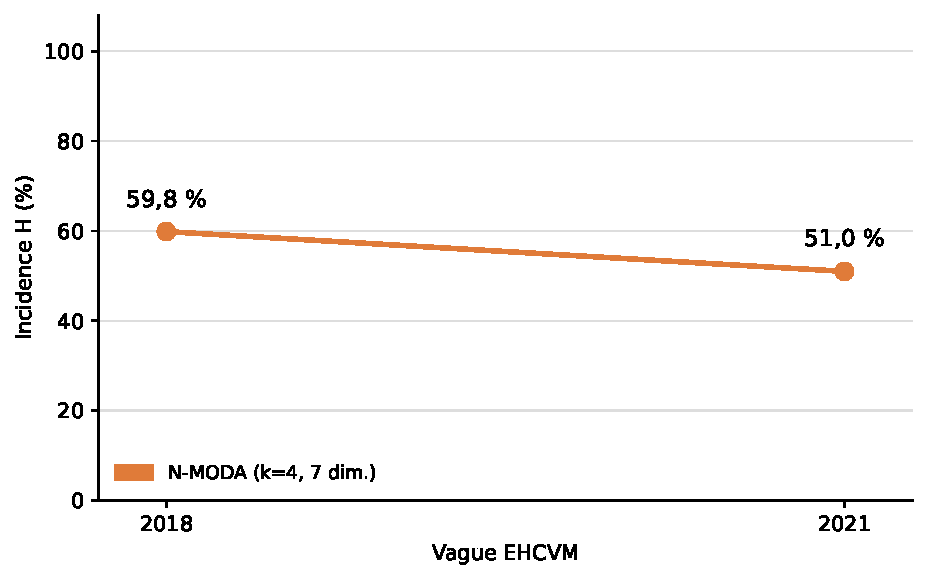
\includegraphics[width=0.85\linewidth]{figures/fig_evolution_ipm.pdf}
  \label{fig:evolution_ipm}

  {\footnotesize \textit{Source :} Calcul de l'auteur, EHCVM.}
\end{figure}

La figure~\ref{fig:evolution_ipm} met en évidence le quasi-parallélisme des
deux trajectoires, qui reculent conjointement, l'écart entre elles se refermant
à peine. Cette comparaison est déclinée groupe d'âge par groupe d'âge dans les
sous-sections~\ref{subsec:age_0_4} à~\ref{subsec:age_15_17}.

Le tableau~\ref{tab:prevalence_dim} décompose les taux de privation par
dimension pour l'ensemble des enfants. La dimension santé (combustible solide
pour cuisiner ou absence d'accès à pied à une structure de santé) est la
privation la plus répandue, touchant environ 97\,\% des enfants aux deux
vagues. Viennent ensuite la nutrition, mesurée par l'échelle FIES (\emph{Food
Insecurity Experience Scale}) de l'insécurité alimentaire vécue, la protection
de l'enfant et le logement inadéquat. Cette dernière dimension est celle qui
s'améliore le plus entre les deux vagues (-$10{,}9$ pp), tandis que l'éducation
progresse de 7,7 points. Cette hausse n'est pas une dégradation~: elle tient
pour l'essentiel au vieillissement du panel, l'indicateur de scolarisation
devenant applicable à des enfants qui étaient trop jeunes en 2018.

\begin{table}[H]
  \centering
  \caption[Taux de privation par dimension MODA (enfants 0-17 ans, \%)]{Taux de privation par dimension MODA (enfants 0-17 ans, \%)\protect\footnotemark}
  \label{tab:prevalence_dim}
  \zebre
  \begin{tabularx}{\linewidth}{|X|c|c|c|}
    \hline
\entete Dimension & EHCVM I & EHCVM II & Variation (pp) \\
    \hline
    Assainissement     & 53,9 & 51,5 & -$2{,}4$ \\ \hline
    Eau                & 23,2 & 18,0 & -$5{,}2$ \\ \hline
    Logement           & 66,4 & 55,5 & -$10{,}9$ \\ \hline
    Nutrition          & 72,2 & 65,9 & -$6{,}3$ \\ \hline
    Santé              & 97,0 & 96,5 & -$0{,}5$ \\ \hline
    Protection de l'enfant & 65,3 & 65,0 & -$0{,}3$ \\ \hline
    Éducation          & 28,8 & 36,5 & $7{,}7$ \\
    \hline
    \hline
    \multicolumn{4}{|c|}{Indice MODA} \\ \hline
    \quad Incidence $H$ (\%)                           & 65,8 & 59,9 & -$5{,}9$ \\ \hline
    \quad Intensité $A$ (\%)                           & 71,2 & 70,6 & -$0{,}6$ \\ \hline
    \quad Indice ajusté $M_0$                          & 0,468 & 0,422 & -$0{,}046$ \\
    \hline
  \end{tabularx}

  {\footnotesize \textit{Source :} Calcul de l'auteur, EHCVM.}
\end{table}
\footnotetext{\textit{Note :} définition détaillée des indicateurs de chaque dimension en annexe~\ref{ann:C}.}

Le tableau~\ref{tab:moda_age} récapitule l'incidence par groupe d'âge de la
période de base. En 2018, les enfants de 5 à 14 ans affichent le taux le plus
élevé (69,8\,\%), du fait des privations éducatives cumulées aux privations de
logement et d'assainissement. Le classement s'inverse en 2021~: cette tranche
enregistre le recul le plus net (-$10{,}7$ pp) et passe sous les deux autres,
tandis que les enfants de 0 à 4 ans en 2018 voient leur incidence augmenter de
2,6 points. Cette hausse est la contrepartie du vieillissement déjà signalé~:
scolarisables en 2021, ces enfants sont désormais évalués sur sept dimensions
au lieu de six, ce qui relève mécaniquement leur probabilité d'atteindre le
seuil de quatre privations.

\begin{table}[H]
  \centering
  \caption{Incidence MODA par groupe d'âge à la période de base : EHCVM I (2018-2019) et EHCVM II (2021-2022)}
  \label{tab:moda_age}
  \zebre
  \begin{tabular}{|l|c|c|}
    \hline
\entete Groupe d'âge en 2018 & \multicolumn{2}{|c|}{$H$ (\%)} \\ \hline

                 & EHCVM I & EHCVM II \\
    \hline
    0-4 ans     & 59,1 & 61,7 \\ \hline
    5-14 ans    & 69,8 & 59,1 \\ \hline
    15-17 ans   & 59,9 & 54,1 \\
    \hline
    Ensemble 0-17 ans & 65,8 & 59,9 \\
    \hline
  \end{tabular}

  {\footnotesize \textit{Source :} Calcul de l'auteur, EHCVM.}
\end{table}

\begin{table}[H]
  \centering
  \caption{Incidence MODA selon le sexe de l'enfant et le statut du ménage, ensemble des enfants (\%)}
  \label{tab:sexe_ensemble}
  \zebre
  \small
  \resizebox{\linewidth}{!}{%
  \begin{tabular}{|l|c|c|c|c|c|c|c|}
    \hline
\entete & \multicolumn{3}{|c|}{EHCVM I (2018-19)} & \multicolumn{3}{|c|}{EHCVM II (2021-22)} & \\ \hline
\entete Sexe de l'enfant & Non-bénéf. & Bénéf. & Écart & Non-bénéf. & Bénéf. & Écart & DD \\
    \hline
    Garçons & 66,0 & 45,7 & -20,3$^{***}$ & 60,4 & 44,9 & -15,5$^{***}$ & 4,8 \\ \hline
    Filles & 68,5 & 53,9 & -14,6$^{***}$ & 61,8 & 47,1 & -14,7$^{***}$ & -0,1 \\
    \hline
  \end{tabular}%
  }

  {\footnotesize \textit{Source :} Calcul de l'auteur, EHCVM. 7\,355 garçons et 7\,278 filles. $^{***}p<0{,}01$.}
\end{table}

Le tableau~\ref{tab:sexe_ensemble} croise le sexe de l'enfant avec le statut
du ménage et la vague, croisement que l'hypothèse H2 appelle directement.
L'avantage des enfants de ménages bénéficiaires existe pour les deux sexes,
mais son évolution diverge~: la double différence descriptive vaut
4,8 points chez les garçons et -0,1 point chez les filles. L'écart de niveau
initial est plus large chez les garçons (20,3 points contre 14,6), et c'est
chez eux seulement qu'il se resserre~; l'estimation d'impact retrouvera ce
contraste sans parvenir à l'établir statistiquement
(section~\ref{sec:discussion}).

\begin{table}[H]
  \centering
  \caption{Incidence MODA selon le quintile de montant reçu, ensemble des enfants (\%)}
  \label{tab:quintile_ensemble}
  \zebre
  \begin{tabular}{|l|r|c|c|c|}
    \hline
\entete Groupe & Médiane reçue & EHCVM I & EHCVM II & DD \\
    \hline
    Non-bénéficiaires & --- & 67,2 & 61,1 & réf. \\ \hline
    Quintile 1 &    29~000 & 68,2 & 69,3 & 7,2   \\ \hline
    Quintile 2 &   110~000 & 61,6 & 61,4 & 5,9   \\ \hline
    Quintile 3 &   325~000 & 56,3 & 51,6 & 1,5   \\ \hline
    Quintile 4 &   780~000 & 37,2 & 32,8 & 1,7   \\ \hline
    Quintile 5 & 2~070~000 & 31,1 & 21,4 & -3,6  \\
    \hline
  \end{tabular}

  {\footnotesize \textit{Source :} Calcul de l'auteur, EHCVM. Montants en FCFA par an.}
\end{table}

Le tableau~\ref{tab:quintile_ensemble} découpe les ménages bénéficiaires
selon le montant annuel reçu, ce que le volet intensité de l'hypothèse H2
appelle. Deux régularités s'en dégagent. L'incidence décroît fortement avec le
montant à chaque vague~: du premier au cinquième quintile, elle passe de
68,2\,\% à 31,1\,\% en 2018 et de 69,3\,\% à 21,4\,\% en 2021. Et le décrochage
relatif aux non-bénéficiaires se concentre sur le bas de la distribution~: la
double différence vaut 7,2 puis 5,9 points dans les deux premiers quintiles,
s'atténue au milieu et devient négative dans le dernier. Les enfants des
ménages recevant les montants les plus faibles sont donc à la fois les plus
privés et ceux dont la situation se dégrade le plus, relativement aux
non-bénéficiaires~; l'estimation retrouvera ce profil décroissant sans
parvenir à l'établir (section~\ref{sec:discussion}).

\subsection{Enfants de 0 à 4 ans}
\label{subsec:age_0_4}

Cette tranche réunit 5\,089 enfants âgés de 0 à 4 ans en 2018-2019, qui en ont
3 à 7 en 2021-2022. Son incidence MODA passe de 59,1\,\% à 61,7\,\%, seule
progression des trois groupes. Cette hausse ne traduit pas une dégradation des
conditions de vie mais l'élargissement du champ de mesure~: l'éducation,
inapplicable à cet âge en 2018, concerne 43,8\,\% d'entre eux en 2021, quand
les six autres dimensions reculent ou stagnent (tableau~\ref{tab:dim_0_4}).

\begin{table}[H]
  \centering
  \caption{Taux de privation par dimension, enfants de 0 à 4 ans (\%)}
  \label{tab:dim_0_4}
  \zebre
  \begin{tabularx}{\linewidth}{|X|c|c|c|}
    \hline
\entete Dimension & EHCVM I & EHCVM II & Variation (pp) \\
    \hline
    Assainissement     & 55,2 & 52,5 & -$2{,}7$ \\ \hline
    Eau                & 25,0 & 19,3 & -$5{,}7$ \\ \hline
    Logement           & 67,6 & 57,9 & -$9{,}7$ \\ \hline
    Nutrition          & 72,2 & 66,2 & -$6{,}0$ \\ \hline
    Santé              & 96,6 & 96,9 & $0{,}3$ \\ \hline
    Protection de l'enfant & 53,1 & 58,4 & $5{,}3$ \\ \hline
    Éducation          & Non applicable & 43,8 & --- \\
    \hline
    \hline
    Incidence MODA ($H$) & 59,1 & 61,7 & $2{,}6$ \\
    \hline
  \end{tabularx}

  {\footnotesize \textit{Source :} Calcul de l'auteur, EHCVM.}
\end{table}

Le profil de privations des tout-petits se distingue sur deux points. La
protection est la moins fréquente des trois tranches en 2018 (53,1\,\% contre
73,0\,\% chez les 5-14 ans), l'indicateur ne combinant à cet âge que
l'absence d'acte de naissance et la séparation parentale, sans le volet
travail des enfants~; elle progresse ensuite de 5,3 points, à mesure que ces
enfants entrent dans le champ de l'indicateur complet. À l'inverse, l'eau et
le logement les touchent davantage que les aînés, ces privations étant
mesurées au niveau du logement et les jeunes enfants vivant dans les ménages
les plus nombreux. La nutrition touche
ici plus de six enfants sur dix aux deux vagues.

\begin{table}[H]
  \centering
  \caption[Taux de privation selon le statut de bénéficiaire, enfants de 0 à 4 ans (\%)]{Taux de privation par dimension selon le statut de bénéficiaire, enfants de 0 à 4 ans (\%)\protect\footnotemark}
  \label{tab:statut_0_4}
  \zebre
  \small
  \resizebox{\linewidth}{!}{%
  \begin{tabular}{|l|c|c|c|c|c|c|c|}
    \hline
\entete & \multicolumn{3}{|c|}{EHCVM I (2018-19)} & \multicolumn{3}{|c|}{EHCVM II (2021-22)} & \\ \hline
\entete Dimension & Non-bénéf. & Bénéf. & Écart & Non-bénéf. & Bénéf. & Écart & DD \\
    \hline
    Assainissement & 56,7 & 36,9 & -19,9$^{***}$ & 54,0 & 33,8 & -20,3$^{***}$ & -0,4 \\ \hline
    Eau & 25,5 & 19,2 & -6,3 & 19,6 & 15,5 & -4,1 & 2,2 \\ \hline
    Logement & 69,1 & 50,0 & -19,1$^{***}$ & 59,2 & 41,8 & -17,4$^{**}$ & 1,7 \\ \hline
    Nutrition & 73,8 & 53,4 & -20,4$^{***}$ & 67,0 & 57,3 & -9,6$^{**}$ & 10,8 \\ \hline
    Santé & 97,1 & 90,7 & -6,4 & 96,7 & 99,1 & 2,4$^{***}$ & 8,8 \\ \hline
    Protection de l'enfant & 53,1 & 54,3 & 1,2 & 58,2 & 60,6 & 2,4$^{*}$ & 1,1 \\ \hline
    Éducation & \multicolumn{3}{|c|}{Non applicable} & 44,1 & 39,1 & -5,0 & --- \\
    \hline
    Incidence MODA ($H$) & 60,7 & 39,6 & -21,1$^{***}$ & 62,9 & 47,6 & -15,2$^{***}$ & 5,9 \\
    \hline
  \end{tabular}%
  }

  {\footnotesize \textit{Source :} Calcul de l'auteur, EHCVM.}
\end{table}
\footnotetext{\textit{Note :} 5\,089 enfants observés aux deux vagues, pondéré par \texttt{hhweight}. \og Écart \fg{} = bénéficiaires moins non-bénéficiaires~; \og DD \fg{} = évolution de cet écart. Significativité de l'écart testée par régression avec erreurs-types clusterisées par grappe~: $^{*}p<0{,}10$, $^{**}p<0{,}05$, $^{***}p<0{,}01$.}

La comparaison selon le statut de bénéficiaire
(tableau~\ref{tab:statut_0_4}) est celle qui intéresse l'évaluation d'impact.
Les tout-petits des ménages bénéficiaires sont nettement moins souvent pauvres
que les autres, 39,6\,\% contre 60,7\,\% en 2018 et 47,6\,\% contre
62,9\,\% en 2021, et l'avantage se lit sur cinq dimensions sur six en 2018. Il
est le plus large en nutrition (20,4 points) et en assainissement
(19,9 points). La protection fait exception et s'inverse~: les tout-petits des
ménages bénéficiaires y sont un peu plus privés, l'absence
d'un parent parti en migration alimentant directement l'indicateur.

C'est surtout l'évolution de cet écart qui retient l'attention. L'avantage des
bénéficiaires se réduit de 21,1 à 15,2 points, soit une double différence
descriptive de 5,9 points, la plus forte des trois tranches. Elle est portée
avant tout par la nutrition, dont l'écart passe de 20,4 à 9,6 points, soit
10,8 points de resserrement à elle seule, et par la santé (8,8 points).
L'estimation d'impact ne produira toutefois de coefficient significatif ni
sur cette tranche ni sur ces dimensions (section~\ref{sec:discussion})~: le
constat descriptif suggère plus qu'il n'établit.

\begin{table}[H]
  \centering
  \caption{Incidence MODA selon le sexe de l'enfant et le statut du ménage, enfants de 0 à 4 ans (\%)}
  \label{tab:sexe_0_4}
  \zebre
  \small
  \resizebox{\linewidth}{!}{%
  \begin{tabular}{|l|c|c|c|c|c|c|c|}
    \hline
\entete & \multicolumn{3}{|c|}{EHCVM I (2018-19)} & \multicolumn{3}{|c|}{EHCVM II (2021-22)} & \\ \hline
\entete Sexe de l'enfant & Non-bénéf. & Bénéf. & Écart & Non-bénéf. & Bénéf. & Écart & DD \\
    \hline
    Garçons & 60,1 & 37,3 & -22,8$^{***}$ & 62,6 & 46,5 & -16,1$^{**}$ & 6,7 \\ \hline
    Filles & 61,3 & 42,3 & -19,0$^{***}$ & 63,2 & 49,0 & -14,2$^{**}$ & 4,8 \\
    \hline
  \end{tabular}%
  }

  {\footnotesize \textit{Source :} Calcul de l'auteur, EHCVM. 2\,606 garçons et 2\,483 filles. $^{**}p<0{,}05$, $^{***}p<0{,}01$.}
\end{table}

La lecture par sexe (tableau~\ref{tab:sexe_0_4}) montre que le resserrement
touche les deux sexes, un peu plus les garçons, dont la double différence
descriptive atteint 6,7 points contre 4,8 chez les filles. Les garçons
partaient de l'incidence la plus basse de la tranche (37,3\,\% en 2018, soit
22,8 points sous leurs homologues de ménages non bénéficiaires) et perdent
un quart de cet avantage en trois ans.

\begin{table}[H]
  \centering
  \caption{Incidence MODA selon le quintile de montant reçu, enfants de 0 à 4 ans (\%)}
  \label{tab:quintile_0_4}
  \zebre
  \begin{tabular}{|l|r|c|c|c|}
    \hline
\entete Groupe & Médiane reçue & EHCVM I & EHCVM II & DD \\
    \hline
    Non-bénéficiaires & --- & 60,7 & 62,9 & réf. \\ \hline
    Quintile 1 &    29~000 & 56,4 & 82,0 & 23,5 \\ \hline
    Quintile 2 &   110~000 & 55,1 & 60,2 & 2,9  \\ \hline
    Quintile 3 &   325~000 & 43,7 & 45,8 & -0,1 \\ \hline
    Quintile 4 &   780~000 & 25,9 & 37,4 & 9,4  \\ \hline
    Quintile 5 & 2~070~000 & 26,7 & 24,4 & -4,5 \\
    \hline
  \end{tabular}

  {\footnotesize \textit{Source :} Calcul de l'auteur, EHCVM. Montants en FCFA par an.}
\end{table}

Chez les tout-petits, le profil du tableau~\ref{tab:quintile_0_4} suit celui
de l'ensemble mais avec un premier quintile nettement détaché~: la double
différence y atteint 23,5 points, contre -4,5 points dans le dernier. Les
effectifs par case sont toutefois réduits, entre 63 et 97 enfants, ce qui
invite à lire le sens du profil plutôt que la valeur de chaque ligne.

\subsection{Enfants de 5 à 14 ans}
\label{subsec:age_5_14}

Les 5-14 ans forment le groupe le plus nombreux, avec 9\,166 enfants, et le
plus exposé en 2018 : leur incidence MODA atteint 69,8\,\%, plus de dix points
au-dessus des 0-4 ans. C'est aussi le groupe dont la situation s'améliore le
plus nettement, l'incidence tombant à 59,1\,\% en 2021, soit un recul de
10,7 points.

\begin{table}[H]
  \centering
  \caption{Taux de privation par dimension, enfants de 5 à 14 ans (\%)}
  \label{tab:dim_5_14}
  \zebre
  \begin{tabularx}{\linewidth}{|X|c|c|c|}
    \hline
\entete Dimension & EHCVM I & EHCVM II & Variation (pp) \\
    \hline
    Assainissement     & 53,4 & 51,1 & -$2{,}3$ \\ \hline
    Eau                & 22,4 & 17,3 & -$5{,}1$ \\ \hline
    Logement           & 65,8 & 54,4 & -$11{,}4$ \\ \hline
    Nutrition          & 72,2 & 65,6 & -$6{,}6$ \\ \hline
    Santé              & 97,1 & 96,2 & -$0{,}9$ \\ \hline
    Protection de l'enfant & 73,0 & 69,1 & -$3{,}9$ \\ \hline
    Éducation          & 44,7 & 32,7 & -$12{,}0$ \\
    \hline
    \hline
    Incidence MODA ($H$) & 69,8 & 59,1 & -$10{,}7$ \\
    \hline
  \end{tabularx}

  {\footnotesize \textit{Source :} Calcul de l'auteur, EHCVM.}
\end{table}

Deux dimensions expliquent la position initiale de cette tranche. La
protection y culmine à 73,0\,\%, l'indicateur combinant à cet âge l'absence
d'acte de naissance, le travail des enfants et la séparation parentale, soit
les trois volets à la fois. L'éducation, mesurée par la non-scolarisation,
touche 44,7\,\% des enfants du groupe, alors qu'elle ne s'applique pas aux
0-4 ans en 2018.

L'éducation explique aussi une bonne part du recul ultérieur~: elle perd
12,0 points, la plus forte baisse de toutes les dimensions et de toutes les
tranches. Une partie de ces enfants a entre-temps dépassé 14 ans et relève
désormais de l'illettrisme et non plus de la scolarisation, indicateur moins
fréquemment en privation. La baisse du logement (-$11{,}4$ pp), elle, est bien
une amélioration des conditions matérielles, commune aux trois tranches.

\begin{table}[H]
  \centering
  \caption[Taux de privation selon le statut de bénéficiaire, enfants de 5 à 14 ans (\%)]{Taux de privation par dimension selon le statut de bénéficiaire, enfants de 5 à 14 ans (\%)\protect\footnotemark}
  \label{tab:statut_5_14}
  \zebre
  \small
  \resizebox{\linewidth}{!}{%
  \begin{tabular}{|l|c|c|c|c|c|c|c|}
    \hline
\entete & \multicolumn{3}{|c|}{EHCVM I (2018-19)} & \multicolumn{3}{|c|}{EHCVM II (2021-22)} & \\ \hline
\entete Dimension & Non-bénéf. & Bénéf. & Écart & Non-bénéf. & Bénéf. & Écart & DD \\
    \hline
    Assainissement & 54,6 & 38,8 & -15,8$^{***}$ & 52,0 & 39,7 & -12,3$^{***}$ & 3,5 \\ \hline
    Eau & 22,8 & 17,7 & -5,2 & 17,5 & 15,1 & -2,4 & 2,8 \\ \hline
    Logement & 66,8 & 53,9 & -12,9$^{***}$ & 55,5 & 41,6 & -14,0$^{**}$ & -1,1 \\ \hline
    Nutrition & 73,2 & 61,8 & -11,4$^{***}$ & 66,1 & 59,5 & -6,5$^{*}$ & 4,9 \\ \hline
    Santé & 97,5 & 92,5 & -5,0$^{*}$ & 95,9 & 99,0 & 3,0$^{***}$ & 8,1 \\ \hline
    Protection de l'enfant & 72,8 & 75,7 & 3,0 & 69,1 & 69,4 & 0,3 & -2,6 \\ \hline
    Éducation & 45,4 & 35,9 & -9,5$^{***}$ & 33,2 & 26,8 & -6,4 & 3,1 \\ \hline
    \hline
    Incidence MODA ($H$) & 71,1 & 54,4 & -16,8$^{***}$ & 60,3 & 45,2 & -15,1$^{***}$ & 1,6 \\
    \hline
  \end{tabular}%
  }

  {\footnotesize \textit{Source :} Calcul de l'auteur, EHCVM.}
\end{table}
\footnotetext{\textit{Note :} 9\,166 enfants observés aux deux vagues, pondéré par \texttt{hhweight}. \og Écart \fg{} = bénéficiaires moins non-bénéficiaires~; \og DD \fg{} = évolution de cet écart. Significativité de l'écart testée par régression avec erreurs-types clusterisées par grappe~: $^{*}p<0{,}10$, $^{**}p<0{,}05$, $^{***}p<0{,}01$.}

Le tableau~\ref{tab:statut_5_14} décline la même comparaison selon le statut
de bénéficiaire. L'avantage des enfants de ménages bénéficiaires est du même
ordre que chez les tout-petits, 54,4\,\% contre 71,1\,\% en 2018 et
45,2\,\% contre 60,3\,\% en 2021, et il se retrouve sur six dimensions sur
sept, protection exceptée. L'éducation le fait apparaître de façon nette~:
35,9\,\% des enfants de ménages bénéficiaires ne sont pas scolarisés, contre
45,4\,\% des autres.

Contrairement aux 0-4 ans, l'écart ne bouge guère entre les deux
vagues~: la double différence descriptive sur l'incidence est de 1,6 point.
Elle reste sensible sur la santé (8,1 points), la nutrition
(4,9 points) et l'assainissement (3,5 points), mais ces mouvements se
compensent en partie avec ceux du logement
(-$1{,}1$ point) et de la protection (-$2{,}6$ points). Les deux groupes
suivent donc des trajectoires quasi
parallèles dans cette tranche, celle qui pèse pourtant le plus lourd dans
l'échantillon.

\begin{table}[H]
  \centering
  \caption{Incidence MODA selon le sexe de l'enfant et le statut du ménage, enfants de 5 à 14 ans (\%)}
  \label{tab:sexe_5_14}
  \zebre
  \small
  \resizebox{\linewidth}{!}{%
  \begin{tabular}{|l|c|c|c|c|c|c|c|}
    \hline
\entete & \multicolumn{3}{|c|}{EHCVM I (2018-19)} & \multicolumn{3}{|c|}{EHCVM II (2021-22)} & \\ \hline
\entete Sexe de l'enfant & Non-bénéf. & Bénéf. & Écart & Non-bénéf. & Bénéf. & Écart & DD \\
    \hline
    Garçons & 69,5 & 50,2 & -19,3$^{***}$ & 59,2 & 44,1 & -15,1$^{**}$ & 4,2 \\ \hline
    Filles & 72,8 & 58,4 & -14,4$^{***}$ & 61,4 & 46,2 & -15,1$^{***}$ & -0,8 \\
    \hline
  \end{tabular}%
  }

  {\footnotesize \textit{Source :} Calcul de l'auteur, EHCVM. 4\,568 garçons et 4\,598 filles. $^{**}p<0{,}05$, $^{***}p<0{,}01$.}
\end{table}

Le croisement par sexe (tableau~\ref{tab:sexe_5_14}) retrouve le contraste
de l'ensemble~: l'écart se resserre chez les garçons (4,2 points) et reste
stable chez les filles (-0,8 point). L'écart de niveau initial est plus
large chez les garçons, et c'est chez eux qu'il se referme.

\begin{table}[H]
  \centering
  \caption{Incidence MODA selon le quintile de montant reçu, enfants de 5 à 14 ans (\%)}
  \label{tab:quintile_5_14}
  \zebre
  \begin{tabular}{|l|r|c|c|c|}
    \hline
\entete Groupe & Médiane reçue & EHCVM I & EHCVM II & DD \\
    \hline
    Non-bénéficiaires & --- & 71,1 & 60,3 & réf. \\ \hline
    Quintile 1 &    29~000 & 73,2 & 64,9 & 2,5   \\ \hline
    Quintile 2 &   110~000 & 64,0 & 62,0 & 8,8   \\ \hline
    Quintile 3 &   325~000 & 62,8 & 54,5 & 2,5   \\ \hline
    Quintile 4 &   780~000 & 42,4 & 29,6 & -2,0  \\ \hline
    Quintile 5 & 2~070~000 & 32,9 & 19,2 & -2,8  \\
    \hline
  \end{tabular}

  {\footnotesize \textit{Source :} Calcul de l'auteur, EHCVM. Montants en FCFA par an.}
\end{table}

Le tableau~\ref{tab:quintile_5_14} montre que la stabilité d'ensemble de cette
tranche recouvre des mouvements contrastés. Les deux premiers quintiles
décrochent, de 2,5 et 8,8 points, tandis que les deux derniers convergent
légèrement vers les non-bénéficiaires~: le profil décroissant selon le
montant se retrouve, atténué, dans cette tranche.

\subsection{Enfants de 15 à 17 ans}
\label{subsec:age_15_17}

Cette tranche ne compte que 378 enfants. Le suivi individuel en est la cause~:
un enfant de 15 à 17 ans en 2018 en a 18 à 20 en 2021 et sort du champ de
l'étude, si bien que seuls subsistent ceux qui avaient tout juste 15 ans à la
première vague. Leur incidence MODA recule de 59,9\,\% à 54,1\,\%.

Cet effectif ne permet pas une analyse comparable à celle des deux autres
tranches. Les résultats sont rapportés pour mémoire, mais les écarts entre
bénéficiaires et non-bénéficiaires n'y sont significatifs sur aucune dimension
à la première vague, et les effectifs par case tombent à quelques dizaines
d'enfants dès que l'on croise le statut avec le sexe ou le montant reçu. C'est
la même limite qui prive l'estimation d'impact de tout coefficient
interprétable sur cette tranche (section~\ref{sec:discussion}).

\begin{table}[H]
  \centering
  \caption[Taux de privation selon le statut de bénéficiaire, enfants de 15 à 17 ans (\%)]{Taux de privation par dimension selon le statut de bénéficiaire, enfants de 15 à 17 ans (\%)\protect\footnotemark}
  \label{tab:statut_15_17}
  \zebre
  \small
  \resizebox{\linewidth}{!}{%
  \begin{tabular}{|l|c|c|c|c|c|c|c|}
    \hline
\entete & \multicolumn{3}{|c|}{EHCVM I (2018-19)} & \multicolumn{3}{|c|}{EHCVM II (2021-22)} & \\ \hline
\entete Dimension & Non-bénéf. & Bénéf. & Écart & Non-bénéf. & Bénéf. & Écart & DD \\
    \hline
    Assainissement & 50,2 & 45,9 & -4,3 & 48,9 & 35,6 & -13,4 & -9,1 \\ \hline
    Eau & 18,4 & 22,9 & 4,5 & 20,5 & 13,3 & -7,2$^{**}$ & -11,7 \\ \hline
    Logement & 65,9 & 65,0 & -1,0 & 51,5 & 39,6 & -11,9$^{*}$ & -10,9 \\ \hline
    Nutrition & 75,4 & 50,6 & -24,8$^{**}$ & 70,1 & 79,7 & 9,5 & 34,3 \\ \hline
    Santé & 99,5 & 97,2 & -2,3 & 98,2 & 100,0 & 1,8 & 4,1 \\ \hline
    Protection de l'enfant & 40,5 & 58,8 & 18,3 & 54,2 & 55,9 & 1,7 & -16,6 \\ \hline
    Éducation & 32,1 & 32,0 & -0,1 & 32,5 & 21,8 & -10,7 & -10,6 \\ \hline
    \hline
    Incidence MODA ($H$) & 59,3 & 64,2 & 4,9 & 55,5 & 43,3 & -12,2 & -17,1 \\
    \hline
  \end{tabular}%
  }

  {\footnotesize \textit{Source :} Calcul de l'auteur, EHCVM.}
\end{table}
\footnotetext{\textit{Note :} 378 enfants observés aux deux vagues, pondéré par \texttt{hhweight}. \og Écart \fg{} = bénéficiaires moins non-bénéficiaires~; \og DD \fg{} = évolution de cet écart. Significativité de l'écart testée par régression avec erreurs-types clusterisées par grappe~: $^{*}p<0{,}10$, $^{**}p<0{,}05$, $^{***}p<0{,}01$.}

Le tableau~\ref{tab:statut_15_17} se distingue de ceux des deux autres
tranches sur un point~: l'avantage de niveau des enfants de ménages
bénéficiaires n'y apparaît pas en 2018, l'incidence y étant même légèrement
supérieure chez les bénéficiaires (64,2\,\% contre 59,3\,\%), sans que l'écart
soit significatif. Seule la nutrition présente un écart net à la première
vague, de 24,8 points. Aucune des évolutions rapportées dans la dernière
colonne ne repose sur des effectifs suffisants pour être interprétée.

\begin{table}[H]
  \centering
  \caption{Incidence MODA selon le sexe de l'enfant et le statut du ménage, enfants de 15 à 17 ans (\%)}
  \label{tab:sexe_15_17}
  \zebre
  \small
  \resizebox{\linewidth}{!}{%
  \begin{tabular}{|l|c|c|c|c|c|c|c|}
    \hline
\entete & \multicolumn{3}{|c|}{EHCVM I (2018-19)} & \multicolumn{3}{|c|}{EHCVM II (2021-22)} & \\ \hline
\entete Sexe de l'enfant & Non-bénéf. & Bénéf. & Écart & Non-bénéf. & Bénéf. & Écart & DD \\
    \hline
    Garçons & 60,9 & 53,3 & -7,7 & 58,3 & 42,0 & -16,4$^{*}$ & -8,7 \\ \hline
    Filles & 57,8 & 77,5 & 19,8 & 52,8 & 45,1 & -7,7 & -27,5 \\
    \hline
  \end{tabular}%
  }

  {\footnotesize \textit{Source :} Calcul de l'auteur, EHCVM. 181 garçons et 197 filles. $^{*}p<0{,}10$.}
\end{table}

Le croisement par sexe (tableau~\ref{tab:sexe_15_17}) illustre cette limite~:
avec moins de deux cents enfants par sexe, dont une minorité dans des
ménages bénéficiaires, aucun écart n'atteint le seuil de 5\,\% à l'une ou
l'autre vague. Le découpage par montant reçu n'est pas rapporté, chacune de
ses cases reposant sur une quinzaine d'enfants.


% 5. Résultats des estimations
\section{Résultats des estimations}
\label{sec:resultats}

Cette section présente les résultats empiriques de la stratégie d'identification
PSM-Double différence. Elle s'organise en trois temps : l'estimation du score de
propension et la vérification de la qualité de l'appariement, la présentation des
estimateurs de double différence brute, et enfin les résultats de l'estimateur PSM-DD
de l'effet moyen du traitement sur les traités (ATT), avec une analyse des impacts
par dimension de la pauvreté.

\subsection{Estimation du score de propension}

\subsubsection{Résultats du modèle probit}

Le score de propension est estimé par un probit au \emph{niveau de l'enfant},
et non du ménage. Ce choix découle de l'unité d'analyse retenue tout au long
du mémoire : c'est la privation de l'enfant qui constitue la variable de
résultat, et deux enfants d'un même ménage n'ont ni le même sexe, ni le même
âge, ni donc les mêmes dimensions MODA applicables. Apparier des ménages
reviendrait à traiter comme identiques des enfants dont les besoins mesurés
diffèrent.

L'échantillon d'estimation est le panel d'enfants suivis entre les deux
vagues, appariés par l'identifiant préchargé décrit en
section~\ref{sec:methodo} (17\,786 enfants, dont 17\,769 utilisés par le
probit). Cette restriction n'est pas une commodité : c'est la seule
construction dans laquelle le poids d'appariement calculé à la période de base
se rapporte au \emph{même} individu à la seconde vague, condition d'une double
différence individuelle.

Les covariables combinent deux niveaux. Celles du ménage à la période de base
reprennent les déterminants des transferts retenus dans la littérature
\parencite{adams2005,gubert2002} : log de la dépense par tête, taille du
ménage, sexe, âge, niveau d'éducation et état matrimonial du chef, milieu et
région de résidence. S'y ajoutent celles de l'enfant : son sexe et son âge.
Toutes sont mesurées avant l'observation des résultats.

\begin{table}[H]
  \centering
  \caption{Modèle probit pour l'estimation du score de propension (EHCVM I, 2018-2019)}
  \label{tab:probit}
  \zebre
  \begin{tabular}{|l|c|c|}
    \hline
\entete Variable & Coefficient & Éc.-t. (cluster) \\
    \hline
    \textit{Caractéristiques de l'enfant} & & \\ \hline
    \quad Sexe féminin                         & $0{,}018$ & $(0{,}024)$ \\ \hline
    \quad Âge de l'enfant (années)             & $0{,}003$ & $(0{,}003)$ \\ \hline
    \textit{Caractéristiques du chef de ménage} & & \\ \hline
    \quad Âge du chef (années)                 & $0{,}005^{**}$ & $(0{,}003)$ \\ \hline
    \quad Chef féminin                         & $0{,}584^{***}$ & $(0{,}085)$ \\ \hline
    \quad Éducation : secondaire gén.~2        & -$0{,}420^{**}$ & $(0{,}195)$ \\ \hline
    \quad Divorcé(e)                           & -$1{,}082^{***}$ & $(0{,}385)$ \\ \hline
    \textit{Caractéristiques du ménage} & & \\ \hline
    \quad Taille du ménage                     & $0{,}048^{***}$ & $(0{,}006)$ \\ \hline
    \quad Log dépense par tête                 & $0{,}583^{***}$ & $(0{,}074)$ \\ \hline
    \quad Milieu rural                         & -$0{,}093$ & $(0{,}079)$ \\ \hline
    \textit{Effets fixes région}               & \multicolumn{2}{|c|}{Oui} \\
    \hline
    Constante                                  & -$9{,}95^{***}$ & $(1{,}031)$ \\
    \hline
    Pseudo-$R^2$ de McFadden                   & \multicolumn{2}{|c|}{$0{,}143$} \\ \hline
    Observations (enfants, panel suivi $t=0$)  & \multicolumn{2}{|c|}{$17\,769$} \\
    \hline
  \end{tabular}

  {\footnotesize \textit{Source :} Calcul de l'auteur, EHCVM. $^{*}p<0{,}10$, $^{**}p<0{,}05$, $^{***}p<0{,}01$~; écarts-types clusterisés par grappe entre parenthèses.}
\end{table}

Le modèle présente un pseudo-$R^2$ de McFadden de 14,3\,\%. Les déterminants
sont conformes à la littérature : la probabilité qu'un enfant vive dans un
ménage bénéficiaire croît fortement avec la dépense par tête ($0{,}58$), la
présence d'une femme à la tête du ménage ($0{,}58$), la taille du ménage
($0{,}05$) et l'âge du chef. Le coefficient de la dépense par tête signale une
sélection positive : ce sont les ménages les moins contraints qui ont pu
financer un départ à l'étranger. Celui du chef féminin reflète la
configuration migratoire typique où l'époux émigré laisse la gestion du ménage
à son épouse, configuration au c\oe{}ur du canal \og absence parentale \fg{}
discuté en section~\ref{sec:discussion}.

Les deux covariables individuelles ne sont en revanche pas significatives : ni
le sexe de l'enfant ($0{,}018$~; $p = 0{,}458$) ni son âge ($0{,}003$~;
$p = 0{,}355$) ne prédisent l'appartenance à un ménage bénéficiaire, ce qui
était attendu puisque le traitement est reçu au niveau du ménage. Leur
présence dans le modèle ne vise pas à améliorer la prédiction mais à garantir
que chaque enfant traité soit comparé à des enfants témoins de même sexe et de
même âge, donc évalués sur les mêmes dimensions MODA.

\subsubsection{Vérification de la qualité de l'appariement}

La figure~\ref{fig:support} représente les distributions du score de propension
des enfants bénéficiaires ($D=1$) et non bénéficiaires ($D=0$). Les deux
distributions se recouvrent sur l'essentiel de leur support ; les enfants
bénéficiaires situés dans la zone de support commun sont tous retenus et
appariés par la méthode des $k$ plus proches voisins (k-NN, $k=4$, avec
remise), pour un panel apparié de 15\,916 observations-enfants.

\begin{figure}[H]
  \centering
  \caption{Distribution du score de propension : enfants de ménages bénéficiaires et non bénéficiaires (EHCVM I, panel suivi)}
  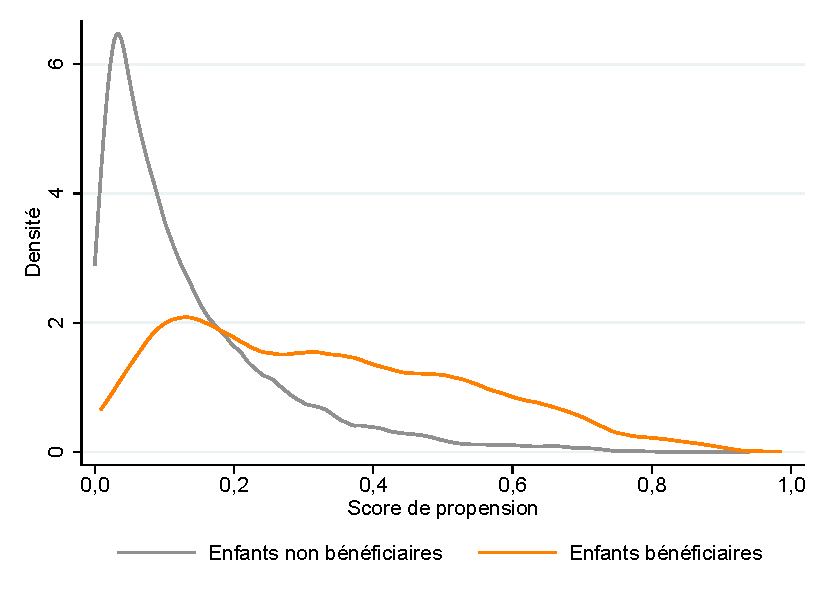
\includegraphics[width=0.85\linewidth]{figures/overlap_panel.pdf}
  \label{fig:support}

  {\footnotesize \textit{Source :} Calcul de l'auteur, EHCVM.}
\end{figure}

Avant appariement, les déséquilibres sont marqués : la différence standardisée
moyenne atteint 12,7\,\%, avec des écarts allant jusqu'à 38\,\% sur le sexe du
chef de ménage et 36\,\% sur la taille du ménage. Le
tableau~\ref{tab:balance} présente le diagnostic d'équilibrage obtenu une fois
l'appariement k-NN effectué : pour chaque covariable, la moyenne chez les
enfants bénéficiaires et chez leurs témoins appariés, la différence
standardisée et le test de Student associé. L'appariement corrige l'essentiel
des déséquilibres : la différence standardisée moyenne tombe à 2,9\,\%
(médiane 2,2\,\%), sous le seuil conventionnel de 10\,\%
\parencite{austin2009}, le pseudo-$R^2$ du probit réestimé sur l'échantillon
apparié passe de 0,143 à 0,006, et aucune différence résiduelle n'est
significative au seuil de 5\,\%. L'équilibrage porte aussi sur les covariables
individuelles, le sexe (SMD résiduelle de -$0{,}4$\,\%) et l'âge
(-$2{,}8$\,\%) de l'enfant.

\begin{table}[H]
  \centering
  \caption[Diagnostic post-appariement de l'équilibrage des covariables (méthode k-NN, niveau enfant)]{Diagnostic post-appariement de l'équilibrage des covariables (méthode k-NN, niveau enfant)\protect\footnotemark}
  \label{tab:balance}
  \zebre
  \small
  \resizebox{\linewidth}{!}{%
  \begin{tabular}{|l|c|c|c|c|c|}
    \hline
\entete Variable & Moyenne traités & Moyenne témoins & SMD (\%) & T-stat & $P>|t|$ \\
    \hline
    Sexe de l'enfant (\% filles) & 0,504 & 0,506 & -0,4 & -0,16 & 0,874 \\ \hline
    Âge de l'enfant (années)     & 6,873 & 6,992 & -2,8 & -1,00 & 0,317 \\ \hline
    Taille du ménage             & 12,45 & 12,25 & 2,7  & 0,46  & 0,644 \\ \hline
    Log dépense par tête         & 13,08 & 13,07 & 1,2  & 0,22  & 0,825 \\ \hline
    Milieu rural (\%)            & 0,391 & 0,392 & -0,2 & -0,04 & 0,970 \\
    \hline
  \end{tabular}%
  }

  {\footnotesize \textit{Source :} Calcul de l'auteur, EHCVM.}
\end{table}
\footnotetext{\textit{Note :} niveau enfant, panel de 17\,786 enfants suivis~; seuil conventionnel~: SMD $< 10\,\%$. Différence standardisée moyenne sur l'ensemble des covariables~: 12,7\,\% avant appariement, 2,9\,\% après.}

\subsection{Impact des transferts sur la pauvreté multidimensionnelle}

\subsubsection{Double différence sans appariement}

À titre de référence, nous estimons d'abord un estimateur de double
différence sans appariement (tableau~\ref{tab:dd_brut}). L'impact estimé est
de $+3{,}2$ points de pourcentage et non significatif ($p = 0{,}167$). Cette
comparaison brute reste toutefois exposée aux différences initiales entre les
deux groupes -- les bénéficiaires sont plus aisés, plus urbains, plus souvent
dirigés par une femme --, d'où le recours à l'appariement.

\begin{table}[H]
  \centering
  \caption[Estimations par double différence (DD brute, sans appariement)]{Estimations par double différence (DD brute, sans appariement)\protect\footnotemark}
  \label{tab:dd_brut}
  \zebre
  \begin{tabular}{|l|c|c|c|}
    \hline
\entete Variable de résultat & ATT$_{\text{DD}}$ & Éc.-t. (cluster) & $p$-valeur \\
    \hline
    Pauvreté MODA ($\hat{H}_{\text{MODA}}$) & $0{,}032$ & $(0{,}023)$ & 0,167 \\
    \hline
  \end{tabular}

  {\footnotesize \textit{Source :} Calcul de l'auteur, EHCVM.}
\end{table}
\footnotetext{\textit{Note :} erreurs-types clusterisées par grappe, $n = 53\,679$~; $\delta$ de $Y_{it} = \alpha + \beta t + \gamma D + \delta(t \times D) + \varepsilon_{it}$.}

\subsubsection{Estimateur par appariement et double différence}
\label{subsec:psmdd}

Le tableau~\ref{tab:psmdd_att} rapporte les estimations de l'ATT par l'estimateur
PSM-DD de \textcite{heckman1997,heckman1998}, qui combine l'appariement par score
de propension et la double différence pour éliminer simultanément les biais de
sélection sur observables et les effets fixes inobservables constants dans le temps.

\begin{table}[H]
  \centering
  \caption[Impact des transferts sur la pauvreté multidimensionnelle : estimateur PSM-DD (ATT)]{Impact des transferts sur la pauvreté multidimensionnelle : estimateur PSM-DD (ATT)\protect\footnotemark}
  \label{tab:psmdd_att}
  \zebre
  \begin{tabular}{|l|c|c|c|}
    \hline
\entete Variable de résultat & ATT & Éc.-t. (cluster) & $p$-valeur \\
    \hline
    \multicolumn{4}{|c|}{\textit{Approche MODA (7 dimensions, $k=4$)}} \\ \hline
    \quad Incidence $\hat{H}_{\text{MODA}}$         & $0{,}053^{*}$ & $(0{,}031)$ & 0,086 \\
    \hline
  \end{tabular}

  {\footnotesize \textit{Source :} Calcul de l'auteur, EHCVM. $^{*}p<0{,}10$.}
\end{table}
\footnotetext{\textit{Note :} appariement k-NN au niveau enfant, erreurs-types clusterisées par grappe, $n = 15\,916$ observations-enfants.}

L'estimateur PSM-DD donne un ATT de $0{,}053$, significatif au seuil de
10\,\% mais non au seuil de 5\,\% ($p = 0{,}086$). Le signe est positif :
entre 2018-2019 et 2021-2022, la privation multidimensionnelle des enfants de
ménages bénéficiaires a reculé \emph{plus lentement} que celle d'enfants
témoins de sexe, d'âge et de profil de ménage comparables, l'écart étant de
l'ordre de 5 points de pourcentage.

Deux conclusions s'imposent. D'abord, l'hypothèse H1 n'est pas validée : les
transferts ne réduisent pas la pauvreté multidimensionnelle des enfants sur
l'horizon observé. Ensuite, la lecture inverse -- celle d'un effet défavorable
-- ne peut être affirmée avec la fermeté qu'exige une conclusion causale :
l'intervalle de confiance à 95\,\% ($[-0{,}8~;~11{,}4]$ points) contient zéro,
et la significativité au seuil de 10\,\% relève d'une présomption plutôt que
d'une démonstration. Cette présomption est toutefois cohérente sur l'ensemble
des spécifications, et la section~\ref{sec:discussion} en examine les canaux
possibles.

La figure~\ref{fig:dd_trajectoires} illustre le mécanisme de la double
différence. Elle représente l'incidence MODA des enfants bénéficiaires et des
témoins appariés aux deux vagues, ainsi que le contrefactuel obtenu en
appliquant la tendance des témoins au niveau initial des bénéficiaires ;
l'écart entre la trajectoire observée des bénéficiaires et son contrefactuel
correspond à l'ATT estimé.

\begin{figure}[H]
  \centering
  \caption{Illustration de la double différence : trajectoires des bénéficiaires,
 	des témoins appariés et contrefactuel (incidence MODA)}
  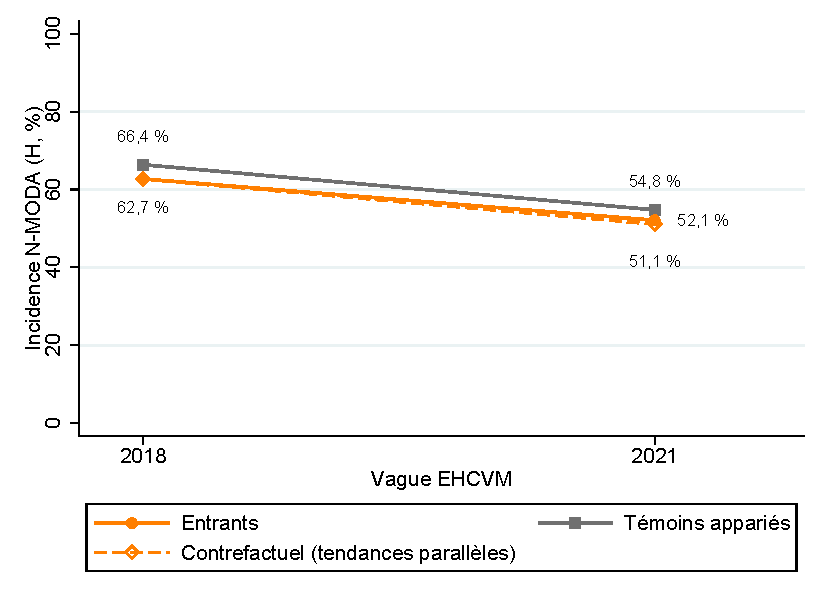
\includegraphics[width=0.85\linewidth]{figures/fig_dd_trajectoires.pdf}
  \label{fig:dd_trajectoires}

  {\footnotesize \textit{Source :} Calcul de l'auteur, EHCVM.}
\end{figure}

\subsubsection{Robustesse au choix de la méthode d'appariement}

Le tableau~\ref{tab:psm_methodes} examine la stabilité des résultats selon la
méthode d'appariement retenue. Les trois algorithmes concordent étroitement :
l'ATT vaut $0{,}053$ pour le k-NN ($p = 0{,}086$), $0{,}060$ pour le noyau
Epanechnikov ($p = 0{,}074$) et $0{,}050$ pour le caliper ($p = 0{,}057$),
tous trois significatifs au seuil de 10\,\% et aucun au seuil de 5\,\%. La
double différence brute, qui ne corrige pas la sélection, donne une valeur
plus faible et non significative ($0{,}032$~; $p = 0{,}167$) : c'est
l'appariement qui fait apparaître l'écart de trajectoire, en neutralisant
l'avantage initial des enfants de ménages bénéficiaires.

\begin{table}[H]
  \centering
  \caption[Sensibilité de l'ATT PSM-DD au choix de la méthode d'appariement]{Sensibilité de l'ATT PSM-DD au choix de la méthode d'appariement\protect\footnotemark}
  \label{tab:psm_methodes}
  \zebre
  \begin{tabular}{|l|c|c|}
    \hline
\entete Méthode d'appariement & ATT (MODA) & $p$-val. \\
    \hline
    k-NN ($k=4$, avec remise)             & $0{,}053^{*}$ & 0,086 \\ \hline
    Noyau Epanechnikov ($h=0{,}06$)       & $0{,}060^{*}$ & 0,074 \\ \hline
    Caliper ($\varepsilon = 0{,}05$, sans remise) & $0{,}050^{*}$ & 0,057 \\ \hline
    DD brute (sans appariement)           & $0{,}032$  & 0,167 \\
    \hline
  \end{tabular}

  {\footnotesize \textit{Source :} Calcul de l'auteur, EHCVM. $^{*}p<0{,}10$.}
\end{table}
\footnotetext{\textit{Note :} erreurs-types clusterisées par grappe, appariement au niveau enfant.}

\subsubsection{Sensibilité au seuil de privation \texorpdfstring{$k$}{k}}
\label{subsec:sensib_k}

Le seuil $k=4$ dimensions sur sept retenu pour déclarer un enfant pauvre est
une convention. Le tableau~\ref{tab:sensib_k} réestime l'ATT en le faisant
varier de $k=3$ à $k=6$, ce qui fait passer l'incidence de 75,1\,\% à
13,3\,\% sur le panel apparié à la période de base. Le signe de l'effet est
positif à chaque seuil et son ampleur décroît avec la sévérité : $5{,}2$ pp à
$k=3$, $5{,}3$ pp à $k=4$, $3{,}4$ pp à $k=5$ et $2{,}9$ pp à $k=6$. La
significativité suit la même pente : l'effet est significatif à 5\,\% pour la
définition la plus inclusive ($p = 0{,}042$), à 10\,\% au seuil de référence
($p = 0{,}086$), et ne l'est plus au-delà.

Cette structure a un sens économique. Les transferts pèsent sur la marge, là
où quelques privations font basculer un enfant de part et d'autre du seuil, et
non sur le noyau des enfants cumulant six ou sept privations, dont la
situation relève de déficits structurels qu'un flux monétaire ne déplace pas.
La conclusion d'ensemble ne dépend donc pas du choix conventionnel de $k=4$ ;
c'est son intensité qui varie.

\begin{table}[H]
  \centering
  \caption[Sensibilité de l'ATT PSM-DD au seuil inter-dimensionnel $k$]{Sensibilité de l'ATT PSM-DD au seuil inter-dimensionnel $k$\protect\footnotemark}
  \label{tab:sensib_k}
  \zebre
  \begin{tabular}{|c|c|c|c|c|}
    \hline
\entete Seuil $k$ & Incidence 2018 (\%) & ATT & Éc.-t. (cluster) & $p$-valeur \\
    \hline
    3 & 75,1 & $0{,}052^{**}$ & $(0{,}026)$ & 0,042 \\ \hline
    4 & 54,4 & $0{,}053^{*}$  & $(0{,}031)$ & 0,086 \\ \hline
    5 & 31,8 & $0{,}034$      & $(0{,}027)$ & 0,205 \\ \hline
    6 & 13,3 & $0{,}029$      & $(0{,}021)$ & 0,175 \\
    \hline
  \end{tabular}

  {\footnotesize \textit{Source :} Calcul de l'auteur, EHCVM. $^{*}p<0{,}10$, $^{**}p<0{,}05$.}
\end{table}
\footnotetext{\textit{Note :} appariement k-NN au niveau enfant, erreurs-types clusterisées par grappe~; l'incidence est pondérée par \texttt{hhweight} sur le panel apparié à $t=0$.}

\subsubsection{Effets par dimension}

\begin{figure}[H]
  \centering
  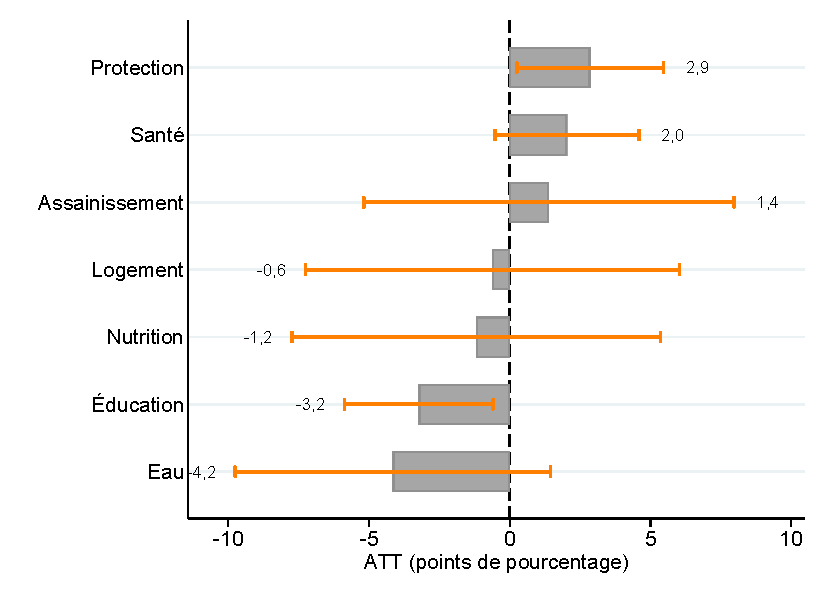
\includegraphics[width=0.85\linewidth]{figures/fig_effets_dim.pdf}
  \caption{Impact des transferts de migrants par dimension MODA (ATT PSM-DD, IC 95\,\%)}
  \label{fig:effets_dim}

  {\footnotesize \textit{Source :} Calcul de l'auteur, EHCVM.}
\end{figure}

L'analyse par dimension (figure~\ref{fig:effets_dim} et
tableau~\ref{tab:effets_dim}) décompose l'ATT global sur les sept dimensions
MODA. Une seule ressort : la \textbf{nutrition}, avec un ATT de $0{,}084$
significatif au seuil de 5\,\% ($p = 0{,}043$). La privation alimentaire des
enfants de ménages bénéficiaires recule 8,4 points plus lentement que celle de
leurs témoins appariés. C'est aussi la dimension la plus directement sensible
au budget courant du ménage, donc celle où un apport monétaire aurait dû se
voir en premier : le résultat va à l'encontre de l'effet attendu.

L'assainissement suit avec $0{,}069$, sans atteindre la significativité
($p = 0{,}109$). Les cinq autres dimensions présentent des coefficients
faibles et non significatifs ; l'éducation est rigoureusement nulle
($-0{,}0001$~; $p = 0{,}995$), et la protection de l'enfant, malgré son
contenu directement lié à l'absence parentale, ne se distingue pas
($0{,}019$~; $p = 0{,}345$).

Le volet dimensionnel de l'hypothèse H2 est donc partiellement validé :
l'effet des transferts n'est pas uniforme entre dimensions, il se concentre
sur la nutrition. Les deux autres volets de H2, relatifs au milieu de
résidence et au sexe de l'enfant, sont examinés en
section~\ref{sec:discussion}.

\begin{table}[H]
  \centering
  \caption[Impact des transferts par dimension MODA (ATT PSM-DD)]{Impact des transferts par dimension MODA (ATT PSM-DD)\protect\footnotemark}
  \label{tab:effets_dim}
  \zebre
  \begin{tabular}{|l|c|c|c|}
    \hline
\entete Dimension & ATT & Éc.-t. (cluster) & $p$-valeur \\
    \hline
    Nutrition            & $0{,}084^{**}$ & $(0{,}042)$ & 0,043 \\ \hline
    Assainissement       & $0{,}069$      & $(0{,}043)$ & 0,109 \\ \hline
    Logement             & $0{,}041$      & $(0{,}041)$ & 0,316 \\ \hline
    Protection           & $0{,}019$      & $(0{,}020)$ & 0,345 \\ \hline
    Santé                & $0{,}010$      & $(0{,}012)$ & 0,400 \\ \hline
    Eau                  & $0{,}003$      & $(0{,}029)$ & 0,928 \\ \hline
    Éducation            & -$0{,}000$     & $(0{,}016)$ & 0,995 \\
    \hline
  \end{tabular}

  {\footnotesize \textit{Source :} Calcul de l'auteur, EHCVM. $^{**}p<0{,}05$.}
\end{table}
\footnotetext{\textit{Note :} appariement k-NN au niveau enfant, erreurs-types clusterisées par grappe.}


% 6. Discussion
\section{Discussion}
\label{sec:discussion}

Cette section discute la validité et la portée des résultats présentés à la
section précédente. Elle comporte quatre volets : les tests de robustesse
(sensibilité au seuil inter-dimensionnel et au choix de la méthode
d'appariement), l'analyse de l'hétérogénéité des effets selon le milieu,
le sexe et l'âge, l'interprétation économique d'un résultat nul, et enfin
les implications pour les politiques publiques.

\subsection{Tests de robustesse}

\subsubsection{Robustesse au champ et à la correction de la sélection}

L'estimation principale porte sur les 14\,633 enfants reliés à eux-mêmes
d'une vague à l'autre, appariés individuellement, une fois écartés les enfants
de ménages bénéficiaires stables ou devenant bénéficiaires en 2021. Ce champ
découle de l'unité
d'analyse et de la définition du traitement, mais il écarte aussi les enfants
nés après 2018, ceux qui atteignent
18 ans et ceux qui quittent le ménage entre les deux passages. La double
différence estimée sans appariement sur l'ensemble des enfants des ménages du
panel, ces derniers compris, donne $0{,}043$~: même signe,
ampleur plus faible, non significatif.

La comparaison des deux chiffres demande une précaution, car ils diffèrent par
deux aspects à la fois~: le champ, restreint ou non aux enfants suivis, et la
correction de la sélection, présente ou absente. Ils ne permettent donc pas
d'isoler l'effet du seul champ. Le second aspect suffit toutefois à rendre
compte du sens de l'écart. La décomposition de l'annexe~\ref{ann:A} montre que
les enfants de ménages bénéficiaires partent d'un niveau de privation
inférieur de 8,0 points à celui de leurs témoins appariés~; sans appariement,
cet avantage initial n'est pas corrigé et l'écart de trajectoire mesuré s'en
trouve mécaniquement atténué.

Trancher entre les deux aspects supposerait d'estimer la double différence
sans appariement sur les seuls enfants suivis, ce que ce travail ne fait pas.
La restriction du champ reste donc une limite du dispositif plutôt qu'un
résultat testé, et elle n'est pas anodine~: les enfants qu'elle écarte sont
précisément ceux dont la situation familiale a changé entre les deux vagues.

\subsubsection{Sensibilité au traitement et à la méthode d'appariement}

Le tableau~\ref{tab:psm_methodes} (section~\ref{subsec:psmdd}) documente la
sensibilité de l'effet estimé à la méthode d'appariement : k-NN ($0{,}051$), noyau Epanechnikov ($0{,}059$) et caliper
($0{,}049$). Les trois algorithmes donnent des effets d'ampleur
voisine, mais seul le noyau franchit le seuil de 10\,\% : l'ampleur est
robuste au choix algorithmique, la significativité ne l'est pas, et les trois
méthodes atteignent une qualité d'équilibrage comparable
(tableau~\ref{tab:balance_global}). La définition alternative
du traitement conduit au même constat. En substituant aux bénéficiaires de
2018 seulement les bénéficiaires stables - recevant un transfert aux deux
vagues, 2\,604 observations-enfants - toujours face aux ménages jamais
bénéficiaires
(23\,580 observations), l'effet tombe à $0{,}023$ et s'éloigne de toute
significativité. Une exposition prolongée aux transferts ne s'accompagne donc
pas d'un écart de trajectoire. Ce design a toutefois ses propres limites, le
traitement y étant déjà en
cours dès 2018 : la première vague n'y mesure pas un niveau pré-traitement.

Enfin, le seuil inter-dimensionnel $k$, que le tableau~\ref{tab:sensib_k}
(section~\ref{subsec:sensib_k}) fait varier sur toute son étendue, module
l'intensité de l'effet : l'ampleur suit une courbe en
cloche, maximale à $k=4$ et retombant de part et d'autre, et la
significativité n'est atteinte qu'à $k=3$. L'écart de trajectoire, pour
autant qu'il existe, se joue au milieu
de la distribution, ni chez les enfants faiblement privés ni dans le noyau des
plus démunis.

\subsection{Analyse de l'hétérogénéité des effets}

\subsubsection{Selon le milieu de résidence}

L'impact des transferts est susceptible de varier selon le milieu de
résidence, le sexe et l'âge de l'enfant. Le tableau~\ref{tab:heterogeneite}
rapporte les effets estimés pour chacun de ces sous-groupes.

\begin{table}[H]
  \centering
  \caption[Hétérogénéité des effets par milieu de résidence, sexe et âge (PSM-DD)]{Hétérogénéité des effets par milieu de résidence, sexe et âge (PSM-DD)\protect\footnotemark}
  \label{tab:heterogeneite}
  \zebre
  \begin{tabular}{|l|c|}
    \hline
\entete Sous-groupe & ATT (MODA) \\
    \hline
    \multicolumn{2}{|c|}{Par milieu de résidence} \\ \hline
    \quad Milieu urbain & $0{,}105^{**}$ \\ \hline
    \quad Milieu rural  & -$0{,}017$     \\ \hline
    \quad Test d'égalité ($p$-valeur) & 0,045 \\
    \hline
    \multicolumn{2}{|c|}{Par sexe de l'enfant} \\ \hline
    \quad Garçons & $0{,}081^{**}$ \\ \hline
    \quad Filles  & $0{,}021$      \\ \hline
    \quad Test d'égalité ($p$-valeur) & 0,131 \\
    \hline
    \multicolumn{2}{|c|}{Par groupe d'âge} \\ \hline
    \quad 0-4 ans   & $0{,}046$      \\ \hline
    \quad 5-14 ans  & $0{,}063^{*}$  \\ \hline
    \quad 15-17 ans & -$0{,}039$     \\ \hline
    \quad Test d'égalité ($p$-valeur) & 0,609 \\
    \hline
  \end{tabular}

  {\footnotesize \textit{Source :} Calcul de l'auteur, EHCVM.}
\end{table}
\footnotetext{\textit{Note :} erreurs-types clusterisées par grappe, poids d'appariement k-NN au niveau enfant. Les groupes d'âge sont ceux de la période de base, l'enfant conservant son groupe aux deux vagues. $^{*}p<0{,}10$, $^{**}p<0{,}05$.}

L'effet est significatif en milieu urbain ($0{,}105$) et absent en milieu
rural (-$0{,}017$), et le test d'égalité rejette cette fois l'homogénéité
($p = 0{,}045$)~: l'écart de 12 points entre les deux coefficients est
lui-même significatif. C'est le résultat d'hétérogénéité le mieux établi de
l'analyse, et le seul volet de l'hypothèse H2 qui soit validé. Il éclaire
aussi l'effet d'ensemble~: le ralentissement de trajectoire, insaisissable en
moyenne, est porté par les enfants des villes, où les bénéficiaires partent
d'un niveau de privation bien plus bas et où la marge de progression est plus
étroite.

\subsubsection{Selon le sexe de l'enfant}

L'effet est significatif chez les garçons ($0{,}081$) et ne l'est
pas chez les filles ($0{,}021$). L'écart entre les deux
coefficients, de six points en faveur des garçons, reste toutefois inférieur
à ce que la précision d'estimation permet de distinguer~: le test d'égalité ne
le sépare pas du bruit ($p = 0{,}131$). Il serait
imprudent d'en conclure que les transferts affectent les garçons et épargnent
les filles sur la seule foi de ces deux coefficients~: selon la spécification
retenue pour l'appariement, c'est tantôt l'un tantôt l'autre sexe qui
franchit le seuil de 5\,\%, et avec 1\,156 enfants traités répartis
en sous-groupes, la puissance disponible ne permet pas de trancher un
écart de cette taille.

Le versant descriptif ne dit pas autre chose (section~\ref{sec:stats}).
L'avantage de niveau des enfants de ménages bénéficiaires est un peu plus
large chez les garçons que chez les filles en 2018, 20,3 points contre 14,6,
et la double
différence descriptive vaut 4,8 points chez les garçons contre -0,1 chez les
filles~: le même contraste apparaît, sans que l'écart soit statistiquement
établi. Le volet de H2 relatif au sexe n'est donc pas validé. La seule
tranche où le descriptif fait apparaître un écart défavorable pour les deux
sexes est celle des 0 à 4 ans, avec 6,7 points chez les garçons et 4,8 chez
les filles.

\subsubsection{Selon les groupes d'âge}

Les groupes d'âge sont ceux de la période de base et suivent l'enfant aux
deux vagues. Un enfant de 3 ans en 2018 en a 6 en 2021~: recalculer son groupe
à chaque vague le ferait changer de sous-groupe en cours de panel, et la
double différence ne comparerait plus le même enfant à lui-même. Un tiers des
observations du groupe des 0-4 ans sont dans ce cas. \og 0-4 ans \fg{} se lit
donc \og âgé de 0 à 4 ans en 2018 \fg{}, ce qui est la lecture pertinente
puisque c'est l'âge à l'exposition qui importe.

Aucune tranche d'âge ne livre d'effet solidement établi. Chez les enfants de
0 à 4 ans, le coefficient vaut $0{,}046$ et n'est pas significatif
($p = 0{,}199$)~; chez les 5-14 ans, il atteint $0{,}063$ et franchit le seuil
de 10\,\% sans atteindre celui de 5\,\%. Le test joint d'égalité des trois
effets ne rejette pas l'homogénéité ($p = 0{,}609$)~: rien ne permet
d'affirmer que l'effet diffère selon l'âge, et le volet de H2 qui s'y rapporte
n'est pas validé. Cette absence de contraste tient pour
partie à la faiblesse des effectifs~: avec 1\,156 enfants traités
répartis sur trois tranches, la puissance disponible ne permet pas de
distinguer des coefficients séparés de quelques points.

Les 15-17 ans échappent en revanche à l'analyse. Un enfant de 15 à 17 ans en
2018 en a 18 à 20 en 2021 et sort du champ de l'étude~: il ne reste que
135 enfants appariés dans ce sous-groupe, contre 1\,511 chez les 0-4 ans et
2\,670 chez les 5-14 ans. Le coefficient obtenu (-$0{,}039$, non significatif)
ne repose sur rien d'exploitable. C'est une limite intrinsèque du suivi
individuel sur trois ans, non un résultat.

\subsubsection{Selon le montant des transferts reçus}
\label{subsec:hetero_montant}

Les trois volets précédents traitent le traitement comme binaire. Or les
montants reçus varient considérablement d'un ménage à l'autre~: parmi les
ménages bénéficiaires de 2018 seulement, la médiane
s'établit autour de 300\,000 FCFA par an et le dernier quintile dépasse
1,2 million (section~\ref{sec:methodo}). Un transfert de 50\,000 FCFA et
un transfert de deux millions ne desserrent pas la même contrainte
budgétaire, et rien n'impose que leurs effets soient de même ampleur. Ce
dernier volet de l'hypothèse H2 examine donc la relation dose-réponse. Les
quintiles sont construits sur la distribution du montant annuel parmi les
ménages bénéficiaires, au niveau du ménage afin que le découpage ne soit pas
déformé par le nombre d'enfants, puis chaque quintile d'enfants traités est
comparé à l'ensemble des enfants témoins appariés. Le tableau
\ref{tab:hetero_montant} rapporte l'effet par quintile ainsi qu'un test continu,
qui estime la pente de l'effet en fonction du logarithme du montant sur les
seuls enfants traités.

\begin{table}[H]
  \centering
  \caption[Hétérogénéité de l'effet selon le montant annuel des transferts]{Hétérogénéité de l'effet selon le montant annuel des transferts\protect\footnotemark}
  \label{tab:hetero_montant}
  \zebre
  \begin{tabular}{|l|c|}
    \hline
\entete Quintile de montant & ATT \\
    \hline
    Q1 (jusqu'à 50~000 FCFA)   & \makecell{$0{,}095$\\$(0{,}079)$} \\ \hline
    Q2 (55~000 à 180~000)      & \makecell{$0{,}082$\\$(0{,}054)$} \\ \hline
    Q3 (200~000 à 480~000)     & \makecell{$0{,}052$\\$(0{,}053)$} \\ \hline
    Q4 (500~000 à 1~200~000)   & \makecell{$0{,}007$\\$(0{,}055)$} \\ \hline
    Q5 (au-delà de 1~230~000)  & \makecell{$0{,}015$\\$(0{,}073)$} \\
    \hline
    \hline
    Pente dose-réponse (log du montant) & \makecell{-$0{,}021$\\$(0{,}020)$} \\
    \hline
  \end{tabular}

  {\footnotesize \textit{Source :} Calcul de l'auteur, EHCVM. $^{*}p<0{,}10$, $^{**}p<0{,}05$.}
\end{table}
\footnotetext{\textit{Note :} appariement k-NN au niveau enfant, erreurs-types clusterisées par grappe, entre parenthèses sous le coefficient. Les quintiles sont définis sur le montant annuel des transferts parmi les ménages bénéficiaires~; chaque quintile est comparé à l'ensemble des témoins appariés. La pente dose-réponse est le coefficient de l'interaction entre la vague et le logarithme du montant, estimé sur les enfants traités.}

Le tableau dessine un gradient sans l'établir. Les coefficients décroissent
des petits montants ($0{,}095$ dans le premier quintile, jusqu'à
50~000 FCFA par an, puis $0{,}082$ dans le deuxième) vers des valeurs
proches de zéro dans les deux derniers quintiles, mais aucun d'eux n'est
significatif, et le test continu ne l'est pas davantage~: la pente de l'effet
en fonction du logarithme du montant vaut -$0{,}021$ ($p = 0{,}308$). Avec
moins de 300 ménages bénéficiaires porteurs d'un montant, répartis en cinq
groupes, la puissance disponible est très faible, et le volet de H2 relatif au
montant n'est pas validé. La structure décroissante des points estimés reste
compatible avec la lecture selon laquelle les petits transferts ne compensent
pas le coût du départ d'un adulte quand les gros le font~: un transfert de
29~000 FCFA par an, montant médian du
premier quintile, représente moins d'un dixième de la dépense annuelle par
tête d'un ménage bénéficiaire, contre plusieurs fois ce montant pour la
médiane du dernier quintile (2,1 millions). Mais cette lecture demeure une
hypothèse, non un résultat.

Deux réserves encadrent la lecture de ce tableau. La première tient à la
mesure du montant, déclaré par le ménage et reconstitué en annualisant le
montant par envoi selon la fréquence rapportée~: l'erreur de mesure y est
vraisemblablement plus forte que sur le statut binaire de bénéficiaire, et
elle atténue mécaniquement toute relation dose-réponse. Que celle-ci
apparaisse malgré cette atténuation en renforce plutôt la crédibilité. La
seconde tient à l'identification~: le montant n'est pas assigné aléatoirement
parmi les bénéficiaires, il dépend des ressources du migrant et des besoins du
ménage. La comparaison entre quintiles ne repose donc pas sur la même
stratégie d'identification que l'estimation principale et s'interprète comme
une association conditionnelle, non comme un effet causal du montant.

\subsection{Interprétation des résultats}

Sur la période 2018-2021, les transferts de migrants ne réduisent pas la
pauvreté multidimensionnelle des enfants sénégalais. L'effet estimé s'établit à
$0{,}051$ et n'est pas significatif ($p = 0{,}103$)~: la trajectoire des
enfants de ménages
bénéficiaires n'est en tout cas pas plus favorable que celle d'enfants témoins
comparables, et le point estimé suggère même un écart défavorable de l'ordre
de 5 points de pourcentage. Ce que les données établissent, c'est que
l'hypothèse d'une réduction de la pauvreté infantile par les transferts est
rejetée. Ce qu'elles suggèrent sans le démontrer, c'est un effet de sens
contraire. Cette présomption s'appuie sur trois indices, à tenir pour ce
qu'ils sont. D'abord la stabilité de l'ampleur~:
les trois algorithmes d'appariement donnent des valeurs voisines, de
$0{,}049$ à $0{,}059$, même si un seul franchit le seuil de 10\,\%. Ensuite
sa localisation~: l'effet est nettement établi en milieu urbain
($0{,}105$, $p = 0{,}020$), où le test d'égalité avec le milieu rural rejette
l'homogénéité, seul résultat d'hétérogénéité qui résiste. Enfin sa position dans
la distribution placebo, au 95,0\textsuperscript{e} centile
(annexe~\ref{ann:A})~: le point estimé est plus grand que ce que produit
la quasi-totalité des réassignations aléatoires du traitement, sans se situer
dans la queue extrême. Il faut en revanche
écarter une lecture erronée. Ce résultat ne signifie pas que
les transferts appauvrissent les enfants. Il signifie qu'appartenir à un ménage
recevant des transferts d'un migrant issu de ce ménage s'accompagne, sur trois
ans, d'une amélioration au mieux équivalente, en ville plus lente, des
conditions de vie de l'enfant. Or ce
statut est indissociable d'un autre événement~: le départ d'un membre du
ménage. Quatre mécanismes, non mutuellement exclusifs, permettent de rendre
compte de ce constat.

Le premier est le coût de l'absence. Les transferts retenus ici ne se
produisent pas sans qu'un adulte ait quitté le ménage, souvent un parent~:
l'expéditeur est par définition un ancien membre parti en migration
(section~\ref{sec:methodo}). Le ménage perd une force de travail, une
capacité de soin et, pour l'enfant, une présence quotidienne
\parencite{cortes2007,davis2016}. L'argent compense la perte de revenu~; il ne
remplace pas l'adulte parti.

Ce mécanisme est plausible, mais les données conduisent à en douter. Le
questionnaire de 2021 précharge chaque membre relevé en 2018 et demande s'il
appartient toujours au ménage, et pour quel motif il l'a quitté. Le motif
distingue explicitement un départ à l'étranger d'un départ ailleurs dans le
pays, ce qui permet de mesurer un fait que le dispositif suppose sans le
vérifier.

Le départ d'un adulte n'est pas propre au groupe traité, et il est même
majoritaire chez les témoins. En excluant les décès et les personnes
recensées à tort en 2018, 53,6\,\% des ménages non bénéficiaires ont vu
partir un membre de 15 ans ou plus entre les deux vagues, contre 66,8\,\%
des bénéficiaires. La différence tient pour l'essentiel à la migration
interne, qui concerne 37,0\,\% des ménages témoins contre 45,3\,\% des
bénéficiaires, alors que le départ vers l'étranger n'en touche
respectivement que 3,6\,\% et 9,8\,\%. Ces ordres de grandeur sont cohérents
avec le profil migratoire du pays, où la migration interne domine largement
les flux~: le recensement de 2013 dénombrait 1,9 million de migrants
internes, dont 43\,\% installés à Dakar \parencite{ansd2018profil}. Le groupe
de comparaison n'est donc pas fait de ménages intacts.

Un second fait pèse davantage encore. Seuls 9,8\,\% des ménages bénéficiaires
enregistrent un départ vers l'étranger pendant la fenêtre d'observation,
alors que tous, par construction du traitement, reçoivent en 2018 un
transfert d'un ancien membre installé hors du pays. Le départ du migrant est
donc, pour l'immense majorité d'entre eux, antérieur à la période étudiée.
Son coût est un effet de niveau, déjà présent en 2018 dans les deux
trajectoires, et c'est précisément ce que la double différence élimine. Ce
qui subsiste dans l'estimation, ce sont les départs survenus entre 2018 et
2021, pour lesquels l'écart entre les deux groupes est de 6,2 points sur
l'étranger et de 8,3 points sur l'interne.

Le coût de l'absence ne peut donc pas porter à lui seul l'écart de
trajectoire suggéré, et il faut le tenir pour une lecture partielle plutôt que
pour l'explication principale.

Le deuxième est la nature de l'usage des fonds. Les transferts sont
massivement affectés à la consommation courante~: 66,7\,\% en 2018-2019 et
68,5\,\% en 2021-2022 relèvent du \og soutien courant \fg{}, contre 3,5\,\%
et 3,7\,\% pour la scolarité et 4,6\,\% et 6,5\,\% pour la santé
(section~\ref{sec:methodo}). Moins d'un dixième des envois est explicitement
fléché vers les dimensions du bien-être de l'enfant que mesure le MODA. Un
flux affecté au budget courant peut soutenir la consommation sans déplacer
les privations structurelles que l'indicateur enregistre.

Le troisième est la contrainte d'offre. Dans les zones à fort déficit
d'infrastructures, les transferts monétaires ne se substituent pas aux
investissements publics collectifs~: le pouvoir d'achat supplémentaire ne
lève pas, à lui seul, les privations d'eau, d'assainissement ou d'accès aux
services de santé \parencite{mansuri2006}. Le fait que la privation en santé
touche 97\,\% des enfants aux deux vagues en est
l'illustration la plus nette.

Le quatrième tient à la marge sur laquelle les transferts opèrent. La
sensibilité au seuil $k$ montre que l'écart de trajectoire se joue chez les
enfants situés au milieu de la distribution des privations, l'effet
s'estompant de part et d'autre du seuil retenu. Le noyau des enfants cumulant
six ou sept privations relève de déficits structurels qu'aucun flux monétaire
privé ne déplace sur trois ans. Ces résultats s'inscrivent enfin dans un débat
empirique contrasté. Si certaines
études trouvent des effets positifs des transferts sur les indicateurs
monétaires de pauvreté \parencite{adams2005,gubert2002}, les effets sur des
indicateurs multidimensionnels structurels sont moins systématiquement
établis, en particulier à court terme \parencite{mansuri2006,cortes2007}. Une
réplication sur la prochaine vague de l'EHCVM, qui allongerait la durée
d'exposition observée, permettrait de trancher entre un coût transitoire
d'ajustement au départ du migrant et un effet durable. Les implications de
politique économique sont développées dans la conclusion générale.


% 7. Conclusion et recommandations
\section*{Conclusion et recommandations}
\addcontentsline{toc}{section}{Conclusion et recommandations}
\markboth{Conclusion et recommandations}{Conclusion et recommandations}

Ce mémoire avait pour objectif d'évaluer l'impact d'une exposition durable
aux transferts de migrants sur la pauvreté multidimensionnelle des enfants
au Sénégal, en exploitant les deux éditions de l'Enquête harmonisée sur
les conditions de vie des ménages. La stratégie d'identification repose
sur l'appariement par score de propension~: l'effet est estimé sur le
nombre de privations de la seconde édition, séparément dans chaque groupe
d'âge, le score incluant le niveau initial de privations de chaque enfant
et les caractéristiques prédéterminées du ménage.

Le résultat principal est un effet protecteur modeste et localisé. Chez
les enfants de 5 à 14 ans, une exposition durable aux transferts réduit le
nombre de dimensions en privation de 0,19, effet significatif au seuil de
10\,\%~; l'effet est de même signe mais imprécis chez les 0 à 4 ans, et
l'effectif des adolescents suivis ne permet aucune conclusion. Cette
réduction est cohérente avec le canal budgétaire des envois, l'écart entre
bénéficiaires et non-bénéficiaires étant le plus marqué sur la sécurité
alimentaire, et elle bute sur les privations d'infrastructure, que le
pouvoir d'achat ne lève pas.

Au regard des hypothèses de départ, H1 est partiellement validée~: une
exposition durable aux transferts réduit la pauvreté multidimensionnelle
des enfants d'âge scolaire, sans que l'effet soit établi aux autres âges.
H2 l'est également en partie~: l'effet se concentre sur les privations qui
répondent au budget courant, la sécurité alimentaire en tête, et croît
fortement avec le montant reçu, seuls les transferts substantiels
réduisant les privations.

\subsection*{Implications de politique économique}

Les résultats obtenus conduisent aux recommandations suivantes, à
l'intention des décideurs politiques. Chacune part d'un fait établi par
l'analyse et en tire une action, de la consolidation du canal par lequel
l'effet protecteur passe jusqu'à la levée des contraintes qui l'empêchent
de s'étendre.

\begin{enumerate}
  \item Consolider le canal alimentaire et l'étendre aux ménages qui
        n'en bénéficient pas. L'insécurité alimentaire est la seule
        dimension où l'effet des transferts est établi, et l'écart entre
        bénéficiaires et non-bénéficiaires y est le plus large de tous
        les indicateurs~: les envois protègent d'abord l'assiette des
        enfants. Les filets sociaux, les cantines scolaires et le suivi
        nutritionnel communautaire devraient donc cibler en priorité les
        enfants de ménages non bénéficiaires des communes d'émigration,
        privés de cet amortisseur privé.

  \item Cibler les enfants de 0 à 4 ans par l'offre de services plutôt
        que par le revenu. Chez les plus jeunes, l'effet protecteur ne se
        matérialise pas sur le nombre total de privations, leurs manques
        dominants, l'acte de naissance et l'environnement sanitaire du
        logement, passant par des démarches et des équipements que
        l'argent reçu ne déclenche pas. La consultation prénatale et
        postnatale, l'appui à l'état civil, la vaccination et les
        structures de garde méritent un renforcement ciblé dans les
        communes d'émigration.

  \item Maintenir les ménages bénéficiaires dans le champ de la
        protection sociale. L'effet protecteur mesuré est modeste, de
        l'ordre d'un cinquième de privation, et l'analyse par montant
        montre que seuls les transferts de la moitié supérieure de la
        distribution, au-delà d'environ 1,25 million de FCFA par an,
        réduisent effectivement les privations. Recevoir de l'étranger ne
        saurait donc valoir exclusion des dispositifs publics, et les
        ménages aux envois modestes doivent être traités, du point de vue
        du ciblage, comme des ménages non couverts.

  \item Augmenter les montants effectivement reçus en réduisant les
        coûts de transaction. Puisque l'effet croît avec le montant, tout
        franc perdu en frais d'envoi est une protection perdue pour
        l'enfant. La concurrence régulatoire sur les frais des canaux
        formels et l'expansion du transfert par téléphonie mobile
        augmenteraient les sommes disponibles et, avec elles, la capacité
        des envois à desserrer le budget courant.

  \item Compléter les transferts par l'offre publique de services de
        base. L'eau, l'assainissement et la santé relèvent
        d'investissements collectifs que le pouvoir d'achat privé ne
        remplace pas, comme le montre la privation de santé, quasi
        universelle dans les deux groupes. Les programmes d'accès
        devraient viser prioritairement les communes rurales
        d'émigration, en tirant parti du réseau associatif des diasporas
        pour amplifier l'effet sur les dimensions les plus rigides.
\end{enumerate}


% ── Annexes ──────────────────────────────────────────────────
\clearpage
\phantomsection
\addcontentsline{toc}{section}{Annexes}
\section*{Annexes}
\begin{appendices}
  % Bandeau : affiche "Annexe A Titre" sans modifier \thesection
  \renewcommand{\ensaebandeaunum}[1]{\ensaebandeau{Annexe~\thesection\quad #1}}
  {\let\clearpage\relax \section{Distribution des privations}
\label{ann:A}

\begin{figure}[H]
  \centering
  \caption{Distribution du nombre de dimensions en privation (EHCVM I et EHCVM II)}
  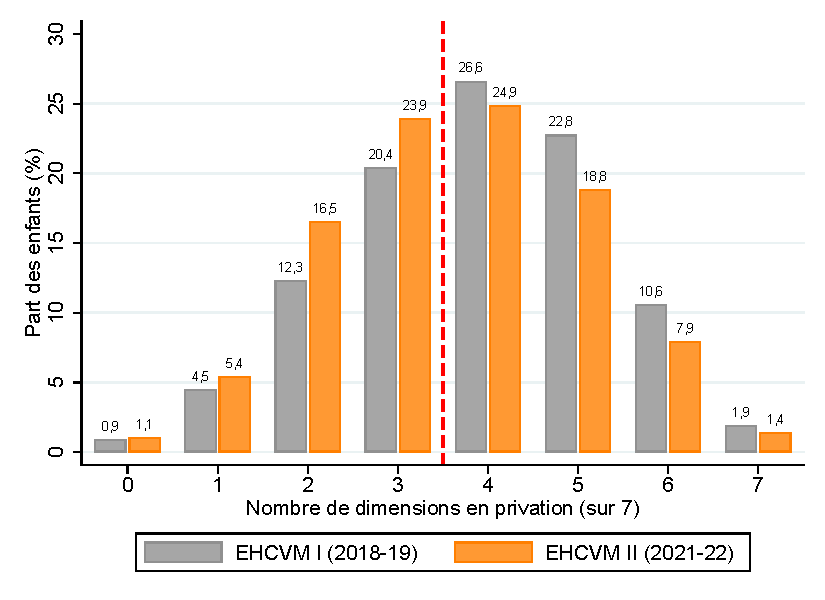
\includegraphics[width=0.85\linewidth]{figures/fig_distrib_dimensions.pdf}
  \label{fig:distrib_dimensions}

  {\footnotesize \textbf{Source :} Calcul de l'auteur, EHCVM.}
\end{figure}
}
  \section{Matrice des indicateurs de pauvreté multidimensionnelle}
\label{ann:C}

Matrice complète des indicateurs de la méthodologie MODA telle qu'appliquée
au Sénégal par l'ANSD et l'UNICEF \parencite{ansd2024}.

\subsection{Principes généraux}

\begin{enumerate}
  \item L'enfant comme unité d'analyse.
  \item Désagrégation par groupe d'âge (0-4, 5-14, 15-17 ans).
  \item Approche union intra-dimension.
  \item Seuil inter-dimensionnel $k = 4$ (sur 7 dimensions).
\end{enumerate}

\subsection{Indicateurs et seuils}

% Tableau pivote a 90 (contenu non flottant, sur sa propre page) pour eviter
% la page blanche que le bloc landscape inserait en twoside. La minipage est
% plus etroite que \textheight pour que le tableau pivote tienne sur la page.
\clearpage
\begin{center}
\rotatebox{90}{%
\begin{minipage}{0.88\textheight}
  \centering
  \begin{threeparttable}
  \footnotesize
  \captionof{table}{Matrice MODA des indicateurs, applicabilité par âge et seuils}
  \label{tab:matrice_nmoda}
  \zebre
  \setlength{\tabcolsep}{4pt}
  \begin{tabular}{|p{2.3cm}|p{3.2cm}|c|c|c|p{6.6cm}|}
    \hline
\entete Dimension & Indicateur & 0-4 & 5-14 & 15-17 & Seuil de privation \\
    \hline
    Assainissement & Toilettes non améliorées & \checkmark & \checkmark & \checkmark & Non conformes aux normes JMP \\ \hline
                   & Partage des toilettes    & \checkmark & \checkmark & \checkmark & Installation partagée \\ \hline
    Eau            & Source non améliorée     & \checkmark & \checkmark & \checkmark & Source non améliorée (une saison ou l'autre) et ménage ne traitant pas son eau \\ \hline
                   & Temps d'accès $\geq 30$ min & \checkmark & \checkmark & \checkmark & 30 minutes ou plus (aller et temps à la source) \\ \hline
    Logement       & Gestion des ordures      & \checkmark & \checkmark & \checkmark & Évacuation non saine \\ \hline
                   & Surpeuplement            & \checkmark & \checkmark & \checkmark & Au moins 4 personnes par pièce \\ \hline
    Nutrition      & Sécurité alimentaire     & \checkmark & \checkmark & \checkmark & Insécurité alimentaire (indice FIES) \\ \hline
    Santé          & Combustible solide       & \checkmark & \checkmark & \checkmark & Bois, charbon ou déchets \\ \hline
                   & Accès à une structure de santé & \checkmark & \checkmark & \checkmark & Pas d'accès à pied à un hôpital ou centre de santé \\ \hline
    Protection     & Absence d'acte de naissance & \checkmark & \checkmark & - & Enfant non enregistré \\ \hline
                   & Travail des enfants      & -          & \checkmark & - & Travail économique ou domestique $\geq$ 1h \\ \hline
                   & Séparation parentale     & \checkmark & \checkmark & \checkmark & Sans ses deux parents biologiques \\ \hline
    Éducation      & Non-scolarisation        & -          & \checkmark & - & Enfant non scolarisé \\ \hline
                   & Illettrisme              & -          & -          & \checkmark & Ne sait ni lire ni écrire \\
    \hline
  \end{tabular}
  \begin{tablenotes}
    \footnotesize
    \item \checkmark~= indicateur applicable au groupe d'âge. - = non applicable.
    \item \textbf{Source :} calcul de l'auteur, adaptation aux choix de l'ANSD
    et de l'UNICEF.
  \end{tablenotes}
  \end{threeparttable}
\end{minipage}}
\end{center}
\clearpage

  \section{Tests statistiques mobilisés et sources}
\label{ann:G}

Cette annexe récapitule les tests et procédures d'inférence utilisés dans le
mémoire, leur logique, la règle de décision et la source méthodologique de
référence. Sauf mention contraire, les erreurs-types sont clusterisées au
niveau de la grappe (unité primaire de sondage).

\subsection{Équilibre des covariables par la différence standardisée moyenne (SMD)}

Avant et après appariement, l'équilibre de chaque covariable $X$ entre
bénéficiaires ($D=1$) et témoins ($D=0$) est mesuré par la différence
standardisée moyenne
\[
  \mathrm{SMD}(X) = \frac{\bar{X}_{1} - \bar{X}_{0}}
       {\sqrt{\tfrac{1}{2}\left(s_{1}^{2} + s_{0}^{2}\right)}},
\]
où $\bar{X}_{d}$ et $s_{d}^{2}$ sont la moyenne et la variance dans le groupe
$d$. Un biais absolu inférieur à 5\,\% après appariement est le seuil
d'équilibre usuellement retenu. La statistique globale (biais moyen,
pseudo-$R^2$ du probit ré-estimé sur l'échantillon apparié) est produite par
la commande \texttt{pstest}. \textit{Sources :}
\textcite{rosenbaum1983,austin2009}.

\subsection{Estimation probit du score de propension}

Le score de propension $e(X)=\Pr(D=1\mid X)$ est estimé par un modèle probit
sur les covariables pré-traitement (taille et composition du ménage,
dépense par tête, milieu, région, sexe, âge et statut matrimonial du chef,
niveau d'instruction). La qualité d'ajustement est appréciée par le
pseudo-$R^2$ et le test du rapport de vraisemblance (LR $\chi^2$).
\textit{Source :} \textcite{rosenbaum1983}.

\subsection{Appariement sur le score de propension}

Trois algorithmes sont comparés~: plus proches voisins ($k=4$, avec remise),
noyau d'Epanechnikov et rayon (caliper, $\epsilon = 0{,}05$, sans
remise), mis en \oe uvre avec \texttt{psmatch2}. La zone de support commun
est imposée pour garantir la comparabilité. \textit{Sources :}
\textcite{rosenbaum1983,heckman1997,heckman1998,caliendo2008}.

\subsection{Estimateur de double différence}

L'effet du traitement sur les traités (ATT) est estimé par la spécification
d'interaction
\[
  Y_{it} = \alpha + \beta\, t + \gamma\, D_i + \delta\,(t \times D_i)
           + \varepsilon_{it},
\]
où $\delta$ est l'ATT. Sur l'échantillon apparié, la régression est pondérée
par les poids d'appariement (PSM-DD)~; le test de significativité de $\delta$
est un test de Student sur la combinaison linéaire $1.t\#1.D$
(\texttt{lincom}). \textit{Sources :} \textcite{card1994} pour la double
différence~; \textcite{heckman1997,heckman1998} pour sa combinaison avec
l'appariement.

\subsection{Erreurs-types clusterisées}

Toutes les inférences reposent sur des erreurs-types robustes à
l'hétéroscédasticité et à la corrélation intra-grappe
(\texttt{vce(cluster grappe)}), qui tiennent compte du plan de sondage à deux
degrés sans recourir aux poids de sondage. \textit{Source :}
\textcite{deaton1997}.

\subsection{Test placebo par permutation}

Pour vérifier l'absence d'effet artefactuel, un faux statut de traitement est
attribué aléatoirement à la même proportion de ménages non-bénéficiaires,
et l'ATT est ré-estimé sur 200 réplications. La position de l'ATT réel dans
la distribution placebo (centile) et la fraction de pseudo-ATT dépassant un
seuil donné mesurent la crédibilité du résultat. La logique est celle des
tests de permutation appliqués à l'inférence causale
\parencite{heckman1997}.

\subsection{Test d'hétérogénéité des effets}

L'égalité des ATT entre sous-groupes (milieu, sexe, groupe d'âge) est testée
par une interaction triple $t \times D \times G$ dans la régression DD~; la
significativité du coefficient d'interaction indique une différence d'effet
entre modalités du facteur $G$. \textit{Source :} \textcite{card1994}.

\subsection{Analyse de l'attrition différentielle}

La comparaison des ménages suivis et perdus entre les deux vagues repose sur
la différence standardisée moyenne (même formule que ci-dessus) et un test de
Student par covariable, afin de vérifier que l'attrition n'introduit pas de
biais de sélection majeur. \textit{Source :} \textcite{rosenbaum2002}.

\end{appendices}

% ── Bibliographie ────────────────────────────────────────────
\clearpage
\phantomsection
\addcontentsline{toc}{section}{Références bibliographiques}
\section*{Références bibliographiques}
\printbibliography[heading=none]

% ── Table des matières complète ──────────────────────────────
\clearpage
\phantomsection
\addcontentsline{toc}{section}{Table des matières}
\tableofcontents

\end{document}
